\documentclass[aspectratio=43]{beamer}
\usepackage[english]{babel}
\usepackage[fntef]{ctex} % invole CJKfntef
\usepackage{ctex}
\usepackage{amsthm}
\usepackage{mathtools}
\usepackage{bm}
\usepackage{physics}
\usepackage{calligra}
\usepackage{csquotes}
\usepackage{tensor}
\usepackage[thicklines]{cancel}
\usepackage{tcolorbox}
\usepackage{pstricks}
\usepackage[backend=biber, bibstyle=nature, sorting=nty, citestyle=numeric-comp]{biblatex} %Custom bibliography
    \addbibresource{bib.bib} %Load references


\DeclareMathAlphabet{\mathcalligra}{T1}{calligra}{m}{n}
\DeclareFontShape{T1}{calligra}{m}{n}{<->s*[2.2]callig15}{}
\newcommand{\scriptr}{\mathcalligra{r}\,}
\newcommand{\boldscriptr}{\pmb{\mathcalligra{r}}\,}
\def\rc{\scriptr}
\def\brc{\boldscriptr}
\def\hrc{\hat\brc}
\newcommand{\ie}{\emph{i.e.}} %id est
\newcommand{\eg}{\emph{e.g.}} %exempli gratia
\newcommand{\rtd}[1]{\ensuremath{\left\lfloor #1 \right\rfloor}}
\newcommand{\dirac}[1]{\ensuremath{\delta \left( #1 \right)}}
\newcommand{\diract}[1]{\ensuremath{\delta^3 \left( #1 \right)}}
\newcommand{\e}{\ensuremath{\epsilon_0}}
\newcommand{\m}{\ensuremath{\mu_0}}
\newcommand{\V}{\ensuremath{\mathcal{V}}}
\newcommand{\prnt}[1]{\ensuremath{\left(#1\right)}} %parentheses
\newcommand{\colch}[1]{\ensuremath{\left[#1\right]}} %square brackets
\newcommand{\chave}[1]{\ensuremath{\left\{#1\right\}}}  %curly brackets

\useoutertheme{infolines}
\useinnertheme{rectangles}
\usefonttheme{professionalfonts}


\definecolor{orange}{HTML}{1f4f94} %背景粉CC0099,蓝色1f4f94,绿色66CC33
\definecolor{gray}{HTML}{FFFFFF}	%底色白
\definecolor{yellow}{HTML}{6633FF}	%f0be52,红色FF0033 %\alert的颜色
\definecolor{lightorange}{HTML}{FF0033} %f19e58
\definecolor{textColor}{HTML}{000000} %黑

\renewcommand{\CancelColor}{\color{orange}}

\makeatletter
\newcommand{\mybox}[1]{%
  \setbox0=\hbox{#1}%
  \setlength{\@tempdima}{\dimexpr\wd0+13pt}%
  \begin{tcolorbox}[colback=orange,colframe=orange,boxrule=0.5pt,arc=4pt,
      left=6pt,right=6pt,top=6pt,bottom=6pt,boxsep=0pt,width=\@tempdima]
    \textcolor{white}{#1}
  \end{tcolorbox}
}
\makeatother

\usecolortheme[named=orange]{structure}
\usecolortheme{sidebartab}
\usecolortheme{orchid}
\usecolortheme{whale}
\setbeamercolor{alerted text}{fg=yellow}
\setbeamercolor{block title alerted}{bg=alerted text.fg!90!black}
\setbeamercolor{block title example}{bg=lightorange!60!black}
\setbeamercolor{background canvas}{bg=gray}
\setbeamercolor{normal text}{bg=gray,fg=textColor}

\setbeamertemplate{footline}
        {
      \leavevmode%
      \hbox{%
      \begin{beamercolorbox}[wd=.333333\paperwidth,ht=2.25ex,dp=1ex,center]{author in head/foot}%
        \usebeamerfont{author in head/foot}\insertshortauthor~~(\insertshortinstitute)
      \end{beamercolorbox}%
      \begin{beamercolorbox}[wd=.333333\paperwidth,ht=2.25ex,dp=1ex,center]{title in head/foot}%
        \usebeamerfont{title in head/foot}\insertshorttitle
      \end{beamercolorbox}%
      \begin{beamercolorbox}[wd=.333333\paperwidth,ht=2.25ex,dp=1ex,center]{date in head/foot}%
        \usebeamerfont{date in head/foot}\insertshortdate{}%\hspace*{2em}

    %#turning the next line into a comment, erases the frame numbers
        %\insertframenumber{} / \inserttotalframenumber\hspace*{2ex} 

      \end{beamercolorbox}}%
  
      \vskip0pt%
    }


\setbeamertemplate{blocks}[rectangle]
\setbeamercovered{dynamic}

\setbeamertemplate{section page}
{
	\begin{centering}
		\begin{beamercolorbox}[sep=27pt,center]{part title}
			\usebeamerfont{section title}\insertsection\par
			\usebeamerfont{subsection title}\insertsubsection\par
		\end{beamercolorbox}
	\end{centering}
}

%\setbeamertemplate{subsection page}
%{
%	\begin{centering}
%		\begin{beamercolorbox}[sep=12pt,center]{part title}
%			\usebeamerfont{subsection title}\insertsubsection\par
%		\end{beamercolorbox}
%	\end{centering}
%}

\newcommand{\hlight}[1]{\colorbox{violet!50}{#1}}
\newcommand{\hlighta}[1]{\colorbox{red!50}{#1}}
\title{概率论与数理统计} %->->->->-> Check hyperref title <-<-<-<-<-
\subtitle{Probability Theory and Mathematical Statistics}
\author[YY]{Yong YANG}
\institute[BUPT]{
	School of Information and Communication Engineering%
	\\%
	Beijing University of Posts and Telecommunications%
} %You can change the Institution if you are from somewhere else
\date{\today}%June 19, 2019}
%\logo{
\includegraphics[width= 0.2\textwidth]{images/a-logo.png}}

\begin{document}
	
	\frame{\titlepage}
	\begin{frame}{目$\quad$次}
	\tableofcontents   
\end{frame}

\begin{frame}{Schedule}
\begin{enumerate}
	\item \alert{概率空间}: 15\%学时
	\item \alert{随机变量(向量)和概率分布}: 11\%学时、14\%学时
	\item \alert{数学期望和方差}: 15\%学时
	\item \alert{特征函数和概率极限定理}: 15\%学时
	\item \alert{样本与抽样分布}: 9\%学时
	\item \alert{参数估计与假设检验}: 9\%学时、12\%学时
\end{enumerate}
\end{frame}

	\begin{frame}{Exercise}
	参考习题,浙大书:
	
	\begin{itemize}
		\item Chap1:1,2,3,4,7,10,11,14,16,20,22,27,30,38,40
		\item Chap2:1,6,13,15,16,19,23,24,25,28,29,30,33,34(1),35(1)
		\item Chap3:1,2,3,5,6,9,10,13,14,16,21,24,30,36
		\item Chap4:4(1),7(2),11,20,24,26(2),33,36
		\item Chap5:2,5,12
		\item Chap6:2,4,6
		\item Chap7:2(3),3(3),8,9,12,16,21,23,25
		\item Chap8:2,6,13,15,18
	\end{itemize}
	选择课后习题的$1/2$至$3/4$,即可达到训练的目的.
    \end{frame}

	\begin{frame}{Bibliography}
	参考书籍:
	\begin{itemize}
		\item Probability:Theory and Examples, Rick Durrett
		\item 高等概率论. 程士宏. 北京:北京大学出版社, 1996.
		\item 测度论讲义. 严加安. 第二版, 北京:科学出版社, 2004.
		\item A First Course in Probability. Sheldon M. Ross. 8th Edition.
		\item A Course in Probability Theory,Chung K L. Second Edition.
		\item 概率论与数理统计. 陈希孺. 合肥,中国科学技术大学出版社, 2009.
		\item 概率论与数理统计教程. 茆诗松等.第二版, 北京,高等教育出版社,2011.2
	\end{itemize}
	\end{frame}
\section{概率空间}

\frame{\sectionpage}

\begin{frame}{概率空间}
\begin{itemize}
	\item 试验与事件
	\item 古典型概率、几何型概率
	\item 概率空间
	\item 概率的性质
	\item 条件概率和乘法公式
	\item 事件的独立性
	\item 全概率公式和Bayes公式
	\item 概率空间的例子
	\item Borel-Cantelli引理
\end{itemize}
\end{frame}

\begin{frame}{Set Theory}
\alert{集合}是数学中最原始的概念.若要给它下定义,不得不引入新的概念来说明它.若要给这些新的概念下定义,又不得不引入另外的新的概念.这样就会导致无休止的讨论.因此,在直观的朴素集合论(naive set theory)中,集合被看成是无需下定义的基本概念.为了方便,我们愿意给集合概念一个直观的描述,但这不是给它下定义.(我们不打算介绍ZFC公理体系等公理化集合论,只介绍比较直观的朴素集合论,对于我们理解这门课,这已足够.)

\begin{itemize}
\item 集合论自19世纪80年代由G.Cantor创立以来,现在已经发展成独立的数学分支.
\item Russell悖论(Russell's paradox 或Russell's antinomy)的出现促使数学家产生了许多改进方案,就是把集合论公理化.

\item 最著名是ZF(Zermelo-Fraenkel)公理集合论体系,及其保守扩张GB(Gödel以及Bernays).
\end{itemize}
\end{frame}

\begin{frame}
\Large\alert{
在此,请同学们相信我们所提到的构造集合的方法都不会导致悖论.集合论中涉及数学基础的那些深层问题,也不会自己跳出来颠覆人们所发展的概率论方法.
}
\\ \hspace*{\fill} \\%空行
在正式开始学习概率论之前,让我们先复习一下集合论的一些简单知识.这些知识构成了概率论语言的基础.我们假定大家对于朴素的集合论已经具有了一定的了解,因此只将这些介绍蜻蜓点水式地简单回顾.
\end{frame}

\begin{frame}{Sets}
\begin{block}{\textbf{Definition}}
\begin{itemize}
\item \alert{集合}就是一些东西的总体.
\item 总体中的东西称为这个集合的\alert{元素}
\item 元素$\omega$是集合$A$的一个元素,称作元素$\omega$属于集合$A$,记作$\omega\in A$或者$A\ni\omega$.
\item 在一个数学问题中,常有这样一个集合$\Omega$,使得我们打算研究的所有对象都是这个特定集合的元素.这个集合$\Omega$常被称为(这个问题的)\alert{空间/全集}(universal set).
\end{itemize}	
\end{block}
\end{frame}

\begin{frame}
	众所周知,一个\alert{集合}(set)就是把一堆\alert{元素}(element)放在一起当作一个整体来看待.当$x$时$A$的元素的时候,我们也称$x$\alert{属于}(belong to)$A$,记为$x\in A$,否则称$x$不属于$A$,记为$x\notin A$.当两个集合相等当且仅当所含元素完全相同.于是证明两个集合$A=B$的标准办法就是去证明\begin{equation}
		x\in A\Longleftrightarrow x\in B.
	\end{equation}
	不含任何元素的集合称为\alert{空集}(empty set),记做$\emptyset$.
	\\ \hspace*{\fill} \\%空行
	但并不是说随便把一堆对象拿出来放在一起就可以构成一个集合,这会导致悖论.比如著名的\alert{Russell悖论}(Russell's paradox或Russell's antinomy)是说,如果定义$X$为“又所有不属于自己的集合构成的集合”,则从$X\in X$就能推出$X\notin X$,反过来从$X\notin X$也能推出$X\in X$,这是自相矛盾的.换言之有些构造集合的方法是安全的,有些则是不安去的,为了避免悖论的产生,无法用安全的方法实现的构造我们都不应当承认它是集合.下面介绍几种常规(即安全的)构造方法.
\end{frame}

\begin{frame}
	一种最常用的构造方法是从一个已知的集合中筛选出满足特定条件的元素,构成新的集合.已知$X$是一个集合,设$P(x)$是一个关于$x$的命题,则$X$中的元素使得命题$P(x)$成立的那些元素$x$就构成一个集合,记为\begin{equation}
		\{x\in X|P(x) \}.
	\end{equation}
	有些时候我们打算研究的对象都是某个特定集合$X$的元素,这时就把$X$称为\alert{全集}(universal set).所以Russell悖论和上述合法构造的差别就在于:悖论里构造的那个东西没有一个全集限定元素的选择范围.
	\\ \hspace*{\fill} \\%空行
	设$A,B$是两个集合,如果$x\in A$蕴含$x\in B$,则称$A$为$B$的\alert{子集}(subset)或者$A$\alert{包含于}(be included in)$B$,并称$B$\alert{包含}$A$,记作$A\subset B$或$B\supset A$.如果$A\subset B$,并且$A\neq B$,则称$A$为$B$的\alert{真子集}(proper subset).
\end{frame}


\begin{frame}
	$X$的全体子集也构成一个集合,称其为\alert{幂集}(power set),记为$2^X$.用这个记号是因为当$X$是恰好有$n$个元素的有限集时,$2^X$是恰好有$2^n$个元素的有限集.
	\\ \hspace*{\fill} \\%空行
	一个所有元素都是集合的集合称为\alert{集合族}(collection of sets).设$\mathcal{A}$是集合族,则可以定义$\mathcal{A}$的所有元素(都是集合)的\alert{交集}(intersection)$\cap\mathcal{A}$以及\alert{并集}(union)$\cup\mathcal{A}$如下:
	\begin{itemize}
		\item $x\in\cap\mathcal{A}$当且仅当$x$是每一个集合$A\in\mathcal{A}$的元素;
		\item $x\in\cup\mathcal{A}$当且仅当存在集合$A\in\mathcal{A}$,使得$x$是$A$的元素.
	\end{itemize}
	
\end{frame}

\begin{frame}
	这里有个小小的问题:如果$\mathcal{A}$不含任何元素,那么如何判断一个元素$x$是不是每个集合$A\in\mathcal{A}$的元素呢?为此我们规定$\cap\emptyset = \emptyset$.
	\\ \hspace*{\fill} \\%空行
	如果集合族$\mathcal{A}$只有两个元素$A$和$B$,则交集和并集就记为$A\cap B$和$A\cup B$.对于一般的集合族,人们也往往喜欢弄出一个指标集$\Lambda$,然后把集合族写成$\{A_{\lambda}\}_{\lambda\in\Lambda}$,并把交集和并集写成$\bigcap_{\lambda\in\Lambda}A_{\lambda}$和$\bigcup_{\lambda\in\Lambda}A_{\lambda}$的样子.请注意,指标集可以是任何集合,而不一定是自然数集或其子集,所以一般来说是不能对指标集应用数学归纳法的.
\end{frame}

\begin{frame}
	交和并的运算满足各自的交换律和结合律,也满足分配律,即
	\begin{itemize}
		\item \begin{equation}
		A\cup\left(\bigcap_{\lambda\in\Lambda}B_{\lambda} \right) = \bigcap_{\lambda\in\Lambda} \left(A\cup B_{\lambda} \right)
		\end{equation}
		\item \begin{equation}
		A\cap\left(\bigcup_{\lambda\in\Lambda}B_{\lambda} \right) = \bigcup_{\lambda\in\Lambda} \left(A\cap B_{\lambda} \right)
		\end{equation}
	\end{itemize}
	两个集合$A,B$的\alert{差集}(difference)定义为\begin{equation}
		A\backslash B = \{x\in A|x\notin B \},
	\end{equation}
	有时候,差集也记做$A-B$.
\end{frame}

\begin{frame}
	差集满足\alert{De Morgan定律}(De Morgan's law)
	\begin{itemize}
		\item \begin{equation}
			B\backslash\left(\bigcap_{\lambda\in\Lambda}A_{\lambda} \right) = \bigcup_{\lambda\in\Lambda}\left(B\backslash A_\lambda\right)
		\end{equation}
		\item \begin{equation}
			B\backslash\left(\bigcup_{\lambda\in\Lambda}A_{\lambda} \right) = \bigcap_{\lambda\in\Lambda}\left(B\backslash A_\lambda\right)
		\end{equation}
	\end{itemize}
	特别地,如果对于我们研究的问题有一个预先取定的全集$X$,则差集$X\backslash A$称为$A$对全集$X$的\alert{余集}或\alert{补集}(complement),记为$A^{c}$.注意,有些文献会习惯使用$\overline{A}$表示$A$的余集,但我们如果也使用这个符号,就会在后面讨论$A$的"闭包"时,会产生歧义,因而此处只使用$A^{c}$来表示$A$的余集.
\end{frame}
\begin{frame}
	\begin{block}{\textbf{Definition}}
		\begin{itemize}
			\item 一个\alert{映射}(map或mapping)$f$是两个集合$X$和$Y$的元素之间的一个对应关系,使得每个$X$的元素$x$都对应唯一一个$Y$的元素$f(x)$.
			\item 我们有时也把映射的定义简写为\begin{equation}
				f:X\rightarrow Y,x\mapsto f(x).
				\end{equation}
			\item 称$X$为$f$的\alert{定义域}(domain),$Y$为$f$的\alert{陪域}(codomain).
			\item 全体$X$到$Y$的映射也构成一个集合,记作$Y^X$.用这个记号是因为当$X$有$m$个元素,$Y$含$n$个元素时,$Y^X$恰好含$n^m$个元素.
		\end{itemize}	
	\end{block}
\end{frame}

\begin{frame}
	注意:幂集$2^\Omega$的元素可以和$\{0,1\}^\Omega$的元素建立起一一对应关系:每一子集$A\subset \Omega$对应的映射就定义为\begin{equation}
		\bm{1}_A:\Omega\rightarrow \{0,1\},\omega\mapsto\left\{
		\begin{aligned}
		1 &,~\omega\in A ;\\
		0  &,~\omega\in \Omega\backslash A.
		\end{aligned}
		\right.
	\end{equation}
		\\ \hspace*{\fill} \\%空行
	如果$y=f(x)$,则称$y$为$x$的\alert{像}(image),称$x$为$y$的一个\alert{原像}(preimage或inverse image).从定义可以看出,每个$x\in X$只能有一个像,但是每个$y\in Y$可以有很多原像,也可以没有原像.$y$的所有原像构成的集合记为$f^{-1}(y)$.如果$A$是$X$的子集,则称\begin{equation}
		f(A) = \{y\in Y|\text{存在} x\in A,\text{使得}f(x)=y\}
	\end{equation}
	为$A$的\alert{像集}(image).
\end{frame}

\begin{frame}
	如果$B$是$Y$的子集,则称\begin{equation}
		f^{-1}(B) = \{x\in X|f(x)\in B\}
	\end{equation}
	为$B$的\alert{原像集}(preimage或inverse image).
		\\ \hspace*{\fill} \\%空行
	不难验证,原像集满足下述简单的规律:
	\begin{itemize}
		\item \begin{equation}
			f^{-1}\left(\bigcap_{\lambda\in\Lambda}A_{\lambda} \right) = \bigcap_{\lambda\in\Lambda}f^{-1}\left(A_{\lambda}\right);
		\end{equation}
		\item \begin{equation}
			f^{-1}\left(\bigcup_{\lambda\in\Lambda}A_{\lambda} \right) = \bigcup_{\lambda\in\Lambda}f^{-1}\left(A_{\lambda}\right);
		\end{equation}
		\item \begin{equation}
			f^{-1}(A\backslash B) = f^{-1}(A) \backslash f^{-1}(B).
		\end{equation}
	\end{itemize}
\end{frame}

\begin{frame}
	但是,像集却完全可能不满足这些规律.
		\\ \hspace*{\fill} \\%空行	
	如果任取两个点$x_1,x_2\in X$,$x_1\neq x_2$蕴含$f(x_1)\neq f(x_2)$,则称$f$为\alert{单射} (injection).如果任取一个$Y$中的点$y$,$f^{-1}(y)\neq\emptyset$,则称$f$是\alert{满射} (surjection).如果$f$既是单射又是满射,则称$f$为\alert{双射} (bijection)或\alert{一一对应} (one-to-one correspondence).有时,也称双射为\alert{可逆映射} (invertible map),因为此时每一个$y\in Y$存在唯一原像,从而可以定义\alert{逆映射} (inverse)
	\begin{equation}
		f^{-1}:Y\to X,
	\end{equation}
	把每个$y\in Y$对应到它关于$f$的那个唯一原像.
\end{frame}

\begin{frame}
	任何集合上都可以定义\alert{恒同映射}(identity)\begin{equation}
		\mathrm{id}_X:X\to X,x\mapsto x.
	\end{equation}
	如果$A\subset X$,则可定义\alert{含入映射}(inclusion),也叫\alert{包含映射}\begin{equation}
		i_A:A\to X,x\mapsto x.
	\end{equation}
	若有两个映射$f:X\to Y$和$g:Y\to Z$,则可以定义\alert{复合映射}(composition)\begin{equation}
		g\circ f:X\to Z,x\mapsto g(f(x))
	\end{equation}
	不难验证,复合应黑色满足下述两个基本性质:
	\begin{itemize}
		\item 如果$g\circ f$是单射,则$f$是单射;
		\item 如果$g\circ f$是满射,则$g$是满射.
	\end{itemize}
\end{frame}

\begin{frame}
	若$X,Y$是两个集合,则全体有序对$(x,y)$(其中$x\in X,y\in Y$)也构成一个集合,称为$X$和$Y$的\alert{笛卡儿积}(Cartesian product)或\alert{直积}(direct product),记作$X\times Y$(英文Cartesian其实是将Descartes(笛卡儿)的名字形容词化之后的结果).也可以类似地定义有限多个集合的直积$X_1\times \cdots \times X_n$,即所有序列$(x_1,\cdots,x_n)$(其中每个$x_j\in X_j$)构成的集合,特别地,$n$个$X$的直积记为$X^n$,例如,实$n$维空间$\mathbb{R}^n = \mathbb{R}\times\cdots\times\mathbb{R}$.
\end{frame}


\begin{frame}
	Cantor最早发明集合论的时候说得很含糊,他说集合是“一些确定的、不同的东西的总体”.他开始想的其实只是实数集$\mathbb{R}$的子集.当然了,他更关心的是无穷子集.他首先发现,一个集合含有无穷多个元素的充分必要条件是它能和自己的一部分一一对应.然后他又提出了比较两个无穷集合所含元素的"个数"谁多谁少的方法.一般集合上这种相当于“个数”的概念称为\alert{基数}(cardinality)或\alert{势}(potency).如果集合$A$和$B$的元素能建立起一一对应,就称它们的基数相同,记为\begin{equation}
		\norm{A} = \norm{B}.
	\end{equation}
	如果$\norm{A}\neq\norm{B}$,但是$A$能和$B$的一部分一一对应,则称$A$的基数小于$B$的基数,记为\begin{equation}
		\norm{A} < \norm{B}.
	\end{equation}
\end{frame}

\begin{frame}
	Cantor很快便证明了$\norm{\mathbb{Q}} = \norm{\mathbb{N}}$,而$\norm{\mathbb{R}} > \norm{\mathbb{N}}$.然后他被一个问题难倒了:是否存在一个集合$A$,使得$\norm{\mathbb{N}}<\norm{A}<\norm{\mathbb{R}}$?Cantor猜想这样的集合不存在,这个猜想被称为连续统假设(因为$\mathbb{R}$的基数被称为连续统),但是他无法证明.
	\\ \hspace*{\fill} \\%空行
	给朴素的集合论想法带来更大打击的是悖论:不加限制地把“满足某种条件的对象”放在一起,有的时候构造出来的东西不能当作集合对待,也就是说,那些对于集合应该自然成立的结论到这里不一定成立,否则会导出自相矛盾的结果.
	\\ \hspace*{\fill} \\%空行
	比如Cantor就发现,把所有的对象放在一起后成一个大全集$\Omega$,$\Omega$就不能当作集合对待.因为否则的话,一方面任何集合的基数都不应该比$\Omega$的基数更大;而另一方面,如果考虑$\Omega$的幂集合$2^\Omega$,又可以像证明$\norm{\mathbb{R}} > \norm{\mathbb{N}}$那样证明$\norm{2^\Omega}>\norm{\Omega}$.这被称为\alert{Cantor悖论}(Cantor's paradox).
\end{frame}

\begin{frame}
	随后Russell(罗素)又发现了更简单直接的\alert{Russell悖论}(Russell's paradox或Russell's antinomy):把所有"不是自己的元素的集合"放在一起构成的那个东西也不能当作集合对待,因为否则的话记这个集合为$\Omega$,则$(\Omega\in \Omega)\Longleftrightarrow (\Omega\notin \Omega)$.
	\\ \hspace*{\fill} \\%空行
	想要避免悖论的发生,就必须要限制构造集合的方法,需要明确知道那些构造方法是安全的,只有那些符合安全规范的方法构造出来的对象才全是集合,才能放心大胆地应用关于集合的那些性质和命题.像前面零个悖论中的$\Omega$就都不算集合了.那然,那些最最基础的构造方法是不是安全是没法证明的,只能把每一条当做一个公理,这样得到的就是集合论的公理系统.历史的发展证明,只要对集合的构造方法加以限制,集合论就可能成为数学的可靠基础.
	
	
\end{frame}

\begin{frame}
最常用的集合论公理系统是ZF及其保守扩张GB(这里Z,F,G,B分别是其发明人Zermelo,Fraenkel,Gödel以及Bernays名字的第一个字母)
\\ \hspace*{\fill} \\%空行
ZF是\alert{Zermelo-Fraenkel集合论}(Zermelo-Fraenkel set theory)的简称,包括九条公理,每条公理是一个逻辑命题.注意ZF系统的所有命题中提到的对象都可以是集合,包括其中提到集合的元素时,这些元素课都可以是集合.仔细观察以下不难发现,这些公理中“某某集合存在”表达的其实都是“某某方式构造是对象算是集合”的意思.
\end{frame}

\begin{frame}
\alert{外延公理}(axiom of extensionality) 如果$x\in X$当且仅当$x\in Y$,则$X=Y$,即集合由其元素完全决定
\\ \hspace*{\fill} \\%空行
\alert{无序对公理}(axiom of pairing)$\forall x,y$,存在集合$\{x,y\}$(无序对),使得$z\in \{x,y\}$当且仅当$z=x$或$z=y$.

Rmk:这里允许$x=y$,此时$\{x,y\}=\{x\}$.能区分$x,y$地位的有序对则定义为集合
\begin{equation}
(x,y) = \{\{x\},\{x,y\}\}.
\end{equation}
\\ \hspace*{\fill} \\%空行
\alert{并集公理}(axiom of union)$\forall \mathcal{A}$,存在集合$\cup\mathcal{A}$,使得$x\in\cup\mathcal{A}$当且仅当存在$A\in\mathcal{A}$满足$x\in A$.

结合无序对公理和并集公理可以归纳定义无序多元组如下:
\begin{equation}
\{x_1,\cdots,x_{n+1} \} = \{x_1,\cdots,x_{n} \} \cup \{x_{n+1}\}.
\end{equation}

\end{frame}

\begin{frame}
\alert{幂集公理}(axiom of power set)$\forall X$,存在集合$2^{X}$(幂集),使得$A\in 2^{X}$当且仅当 $A\subset X$.这里$A\subset X$是逻辑命题
\begin{equation}
\forall x\in A\Rightarrow x\in X
\end{equation}
(即$A$是$X$的子集)的简写.
\\ \hspace*{\fill} \\%空行
\alert{分离公理}(axiom schema of separation或axiom schema of specification) 任取集合$X$以及关于$x$的命题$P(x)$,存在集合$A$使得$x\in A$当且仅当$x\in X$并且$P(x)$成立.集合$A$通常记为$\{x\in X|P(x)\}$.

结合分离公理和并集公理,就可以把交集定义为
\begin{equation}
\cap \mathcal{A} = \{x\in\cup\mathcal{A}|\forall A\in\mathcal{A},x\in A \}.
\end{equation}
\end{frame}

\begin{frame}
注意到当$x\in X,y\in Y$时,前面定义的有序对$(x,y)$其实是一个由$X\cup Y$的子集构成的集合,这样的集合是$2^{X\cup Y}$的子集,也就是$2^{(2^{X\cup Y})}$的元素,因此利用分离公理,可以把直积(direct product)定义为
\begin{equation}
X\times Y = \{ z\in 2^{(2^{X\cup Y})}| \exists x\in X,y\in Y,\text{使得}z=(x,y) \}.
\end{equation}
直积也称作笛卡儿积(Cartesian product),其中英文Cartesian其实是将Descartes(笛卡儿)的名字形容词化之后的结果.

每个从$X$射到$Y$的映射$f:X\rightarrow Y$可以用它在$X\times Y$中的函数图像来刻画,因此也不需要添加新的公理,就可以把从$X$打到$Y$的映射定义为集合
\begin{equation}
Y^X = \{f\in 2^{X\times Y} | \forall x\in X,\text{存在唯一}\ y\in Y\ \text{使得}(x,y)\in f \}
\end{equation}
的元素.并且此时如果$(x,y)\in f$,则把$y$记为$f(x)$.
\end{frame}

\begin{frame}
\alert{空集公理}(axiom of empty set) 存在集合$\emptyset$(空集),使得$\forall x,x\notin \emptyset$.

由外延公理可以知道空集是唯一的.你也许会认为空集公理是多余的,因为有了分离公理可以随便取个集合,再取一个该集合中元素永远不满足的性质,然后就可以构造出空集来了,比如说$\emptyset=\{x\in A|x\notin A\}$.很多的书籍上也确实是这么写的,但是这实际上依赖于另外的一条其它公理中没有提到的假设:在这个世界上确实至少存在着那么一个集合$A$.缺少这个假设,形式逻辑的推理过程就没有了起点.当然,也有群体认为下面的一条公理"无穷公理"本身就包含了一定存在一个空集的意思.
\end{frame}

\begin{frame}
\alert{无穷公理}(axiom of infinity) 存在一个集合$\omega$(含有无穷多个元素的集合),使得$\emptyset\in\omega$,并且$x\in\omega$蕴含$x\cup\{x\}\in\omega$.

在集合论中,每个自然数$n$被归纳地定义成一个恰好有$n$个元素的特殊集合:
\begin{equation}
0=\emptyset,1=\{0\},\cdots,n+1=\{0,\cdots,n\} = n\cup\{n\}.
\end{equation}	

比较一下这个定义和上述无穷公理不难看出,自然数集$\mathbb{N}$就是满足无穷公理的最小集合.有趣的是关于自然数的加减乘除运算的各种基本性质都可以从这个定义以及ZF系统的其它公理推导出来.有了自然数之后当然也可以定义整数和有理数,并把数学分析中定义实数的方法(比如Cauchy序列或者Dedekind分割等等)也改写成符合ZF系统的形式.
\end{frame}

\begin{frame}
\alert{替换公理}(axiom schema of replacement)任取集合$X$以及关于$x,y$的逻辑命题$R(x,y)$,如果$R$满足$\forall x\in X$,存在唯一$y$使得该命题成立,则存在集合$Y$,使得$y\in Y$当且仅当存在一个$x\in X$使得$R(x,y)$成立.
\\ \hspace*{\fill} \\%空行
如果我们把$R(x,y)$理解成一个映射$f:x\mapsto y$,那么替换公理构造的$Y$其实就是$X$的象集$f(X)$.
\\ \hspace*{\fill} \\%空行
\alert{正则公理}(axiom of regularity)任取非空集合$X$,其中元素关于$\in$关系存在一个极小元素,即存在$x\in X$,使得$\forall y\in X,y\notin x$.
\\ \hspace*{\fill} \\%空行
注意:极小元素的选取并不一定唯一,也不一定是最小元素.有趣的是,任取两个自然数$m$和$n$,$m<n$当且仅当按照前述公理化定义把它们当作集合看待时$m\in n$.因此,这最后一条公理给出了\alert{数学归纳法}(mathematical induction)的一种新的理解:要想证明一系列命题$P_n$对任意$n\in\mathbb{N}$都成立,可以取$X=\{ n\in\mathbb{N}|\text{命题}P_n\text{不成立} \}$,则$X$一定含有一个极小元素$m$,从而任取自然数$i<m$,命题$P_i$成立.于是如果我们能从$P_0,\cdots,P_{m-1}$成立推导出命题$P_m$成立,就完成了证明.
\end{frame}


\begin{frame}
ZF是集合论的公理化体系中最简单可靠的一个.当然,简单可靠的代价就是应用上的局限性.有许多数学中的著名论断都需要在ZF之外再添加一条选择公理才能推推导出来.
\\ \hspace*{\fill} \\%空行
\alert{选择公理}(axiom of choice)任取一个由两两不相交的集合构成的集合族$\mathcal{A}$,存在一个集合$C$,它与$\mathcal{A}$的每个元素(元素是集合)都恰好交于一点.
\\ \hspace*{\fill} \\%空行
选择公理的一个简单推论是:任取一个集合族$\mathcal{A}$(不一定两两不交),存在一个映射$f:\mathcal{A}\mapsto\cup\mathcal{A}$,使得$\forall A\in\mathcal{A},f(A)\in A$.换言之,允许同时在集合族$\mathcal{A}$的每个元素(集合)里选择一个元素.


\end{frame}


\begin{frame}
选择公理是一个饱受争议的公理,数学家们一方面对于是否应该允许“同时”进行无穷多项的构造提出了强烈的质疑,另一方面又利用它证明了很多虚无缥缈、无法构造的东西存在.比如线性代数中任意线性空间中基的存在性,或者抽象代数中任意环的极大理想的存在性,或者实变函数(测度论)中不可测集的存在性,或者泛函分析中的Hahn-Banach定理,它们的证明过程中都直接或者间接地用到了选择公理,或者用到了在ZF中与选择公理等价的良序定理或Zorn引理.
\\ \hspace*{\fill} \\%空行
值得一提的是与不可测集的存在性相关的一个著名的结论,人们称之为\alert{Banach-Tarski悖论}(Banach-Tarski paradox).这个悖论大意是说,如果承认选择公理正确,则可以证明存在三维欧氏空间中的一族有限多个互不相交的子集,它们并起来是一个半径为$1$的实心球,但是把每个子集只进行一些旋转和平移,还可以在新的位置上保持互不相交地重新拼出两个半径为$1$的实心球.也就是将神话里的"分身术"找到了数学依据!这看上去显然是非常不符合常识的,这个结论也曾经一度被认为是选择公理不成立的直接证明,因此它才被称为"悖论"而不是"定理".
\end{frame}


\begin{frame}
当然,这个结论在逻辑上并没有任何矛盾,它只是和我们从多面体体积那里得来的常识相矛盾,有什么理由认为这些常识对于那些复杂得不可想象的子集也应该正确呢?今天的大部分数学家都倾向于站在选择公理一边,也就是说,当我们把一大堆没有体积的点胡乱堆在一起的时候,不应当假定这堆点的"体积"就一定符合积木方砖那种东西带给我们的几何常识.只不过在每一个需要用到选择公理的结论上,数学家们都会特意标注一下,省得将来反悔的时候不知道该丢弃些什么.我们也会这样处理.当然,对于本课的主要内容来说,ZF已经足够应用了.

\end{frame}

\begin{frame}
有趣的是,即使是用ZF加上选择公理构成所谓的ZFC,依然解决不了最初难道Cantor的连续统假设,或者说已经解决了,却不是Cantor想要的答案.Gödel在1940年证明了从ZFC出发不可能证明连续统假设是错误的,而Cohen则在1963年证明了从ZFC出发不可能证明连续统假设是正确的.
\end{frame}

\begin{frame}{Cantor-Bernstein 定理}
	
\end{frame}

\begin{frame}{集合系}
	集合系就是由集合组成的集合.在本课中可能用到的集合系有$\pi-\text{系}$、半环、半代数、环、代数、$\sigma-\text{环}$、$\sigma-\text{代数}$、单调系、$\lambda-\text{系}$等.这些集合系中最重要的是\alert{$\sigma-\text{代数}$},下面一一介绍这些集合系.
	\\ \hspace*{\fill} \\%空行
	\alert{$\pi-\text{系}$}:如果$X$上的非空集合系$\mathcal{P}$对交运算封闭,
	
	即\begin{equation}
		\forall A,B\in\mathcal{P} \implies AB\in\mathcal{P}.
	\end{equation} 
	则称$\mathcal{P}$为$\pi-\text{系}$.
	
	例:$\mathcal{P}_\mathbb{R} = \{(-\infty,a]|a\in\mathbb{R}  \}$对有限交的运算封闭,因而组成实数空间$\mathbb{R}$上的$\pi-\text{系}$.
\end{frame}

\begin{frame}
	\alert{半环}:满足下列条件的$\pi-\text{系}~\mathcal{S}$称为半环
\end{frame}

\begin{frame}{集合系之间的关系}
\Large
\begin{tabular}{ccccc}
	$\sigma-\text{代数}$ & $\Longleftrightarrow$ & $\pi-\text{系}$ & $+$ & $\lambda-\text{系}$ \\
	~ & ~ & ~ & ~ & $\Downarrow$ \\
	~  & $\Longleftrightarrow$ & 代数 & $+$ & 单调系 \\
\end{tabular}
\\ \hspace*{\fill} \\%空行
\hspace*{\fill} \\%空行
\begin{tabular}{ccccccc}
	$\sigma-\text{代数}$ & $\Longrightarrow$ & 代数 & $\Longrightarrow$ & 半代数 & ~ & ~ \\
	$\Downarrow$ & ~ & $\Downarrow$ & ~ & $\Downarrow$ & ~ & ~ \\
	$\sigma-\text{环}$ & $\Longrightarrow$ & 环 & $\Longrightarrow$ & 半环 & $\Longrightarrow$ & $\pi-\text{系}$
\end{tabular}
\end{frame}

\begin{frame}{测度论中的典型方法}
	在测度论和概率论中,为了证明一个关于可测函数的命题,常常分解为如下几个比较容易的步骤进行:
	\begin{itemize}
		\item (1)证明该命题对最简单的函数——\alert{示性函数}成立.
		\item (2)证明该命题对非负简单函数——\alert{示性函数的线性组合}成立.
		\item (3)证明该命题对非负可测函数——\alert{非降的非负简单函数列的极限}成立.
		\item (4)证明该命题对一般的可测函数——两个非负可测函数,即它的\alert{正部和负部之差}成立.
	\end{itemize}
	按上述步骤证明命题的方法叫做测度论中的\alert{典型方法}.典型方法符合人们的认识过程,是一种具有普遍意义、行之有效的方法,必须熟练掌握.
\end{frame}


\section{相位噪声和I/Q不平衡模型}
    
    \frame{\sectionpage}
    
    \begin{frame}{\textbf{I/Q不平衡模型}}
   		\begin{block}{理想情况下:给定基带I/Q信号$x(t) = x_I(t)+jx_Q(t)$}
   		\begin{itemize}
   			\item 上变频得到$x_p(t) = x_I(t)\cos(2\pi f_ct) - x_Q(t)\sin(2\pi f_ct)$
   			\item 下变频还原到$x(t) = x_I(t)+jx_Q(t)$.
   		\end{itemize}
   		\end{block}
   	
   		同向和正交两路中, 其相对幅度可能发生不该有的变化. 这会带来我们的 I/Q 不平衡现象.
   	
	\end{frame}
    
    \begin{frame}{\textbf{I/Q不平衡模型}}
    上变频和下变频的过程中,都会带来I/Q不平衡.
    \begin{block}{带有I/Q不平衡时:对基带I/Q信号$x(t) = x_I(t)+jx_Q(t)$}
    	\begin{itemize}
    		\item 上变频得到$\tilde{x}_p(t) = \alpha_{I,tx}x_I(t)\cos(2\pi f_ct) - \alpha_{Q,tx}x_Q(t)\sin(2\pi f_ct)$
    		\item 下变频得到$\tilde{x}(t) = \frac{\alpha_{I,rx}+\alpha_{Q,rx}}{2}x(t) + \frac{\alpha_{I,rx}-\alpha_{Q,rx}}{2}x^*(t)$.
    	\end{itemize}
    \end{block}
    
   	该信号的频谱中产生了一个镜像的频率干扰
   	\begin{equation}
   		\tilde{X}(f) = \frac{\alpha_{I,rx}+\alpha_{Q,rx}}{2}X(f) +  \frac{\alpha_{I,rx}-\alpha_{Q,rx}}{2} X^*(-f)
   	\end{equation}
    
\end{frame}
    
    \begin{frame}{\textbf{I/Q不平衡模型}}
    	\begin{columns}[T] % align columns
    		\begin{column}<0->{.40\textwidth}
    			\begin{figure}[thpb]
    				\centering
    				\resizebox{1\linewidth}{!}{
    					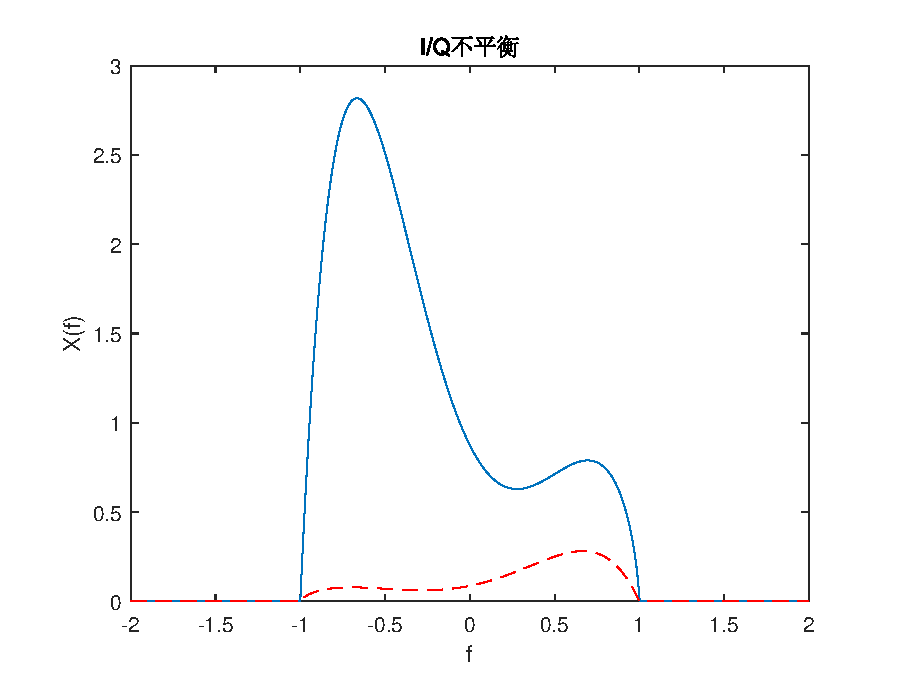
\includegraphics{images/IQ.eps}
    				}
    				%\includegraphics[scale=1.0]{figurefile}
    				$\quad$\caption{I/Q不平衡带来的镜频干扰}
    				\label{fig:campus}
    			\end{figure}
    		\end{column}%
    		\hfill%
    		\begin{column}<0->{.5\textwidth}
    			\begin{itemize}
    				\item 实际的 OFDM系统的上、下变频模块中,这种I/Q不平衡的效应则将会影响镜像位置处的子载波信道中的信号
    				\item I/Q不平衡效应还会使我们错误地估计需要去耦合的那部分发送信号,从而导致自干扰消除后仍然有一部分自干扰残余的出现. 
    			\end{itemize}
    		\end{column}%
    	\end{columns}
	\end{frame}

	\begin{frame}{\textbf{相位噪声模型}}
		\begin{block}{自激(FRO)振荡器模型的相位噪声假定为一个布朗运动}
			\begin{itemize}
				\item 相位噪声的复数振荡器可以描述为$\alpha_{OSC}(t) = e^{j2\pi f_ct}e^{j\phi(t)}$
				\item 相位噪声过程描述为$\phi(t) = \sqrt{c}B(t)$,其中$B(t)$是标准布朗运动
			\end{itemize}
		\end{block}
		\centering
		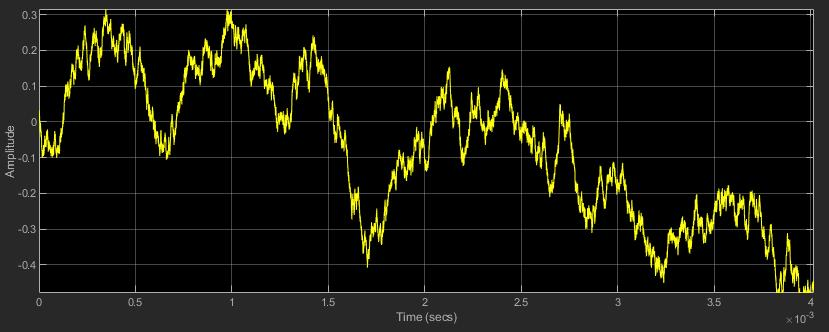
\includegraphics[width = 0.7\textwidth]{images/Ref2Fig2.jpg}
    \end{frame}

	\begin{frame}{\textbf{相位噪声模型}}
		\begin{columns}[T] % align columns
			\begin{column}<0->{.40\textwidth}
				\begin{figure}[thpb]
					\centering
					\resizebox{1\linewidth}{!}{
						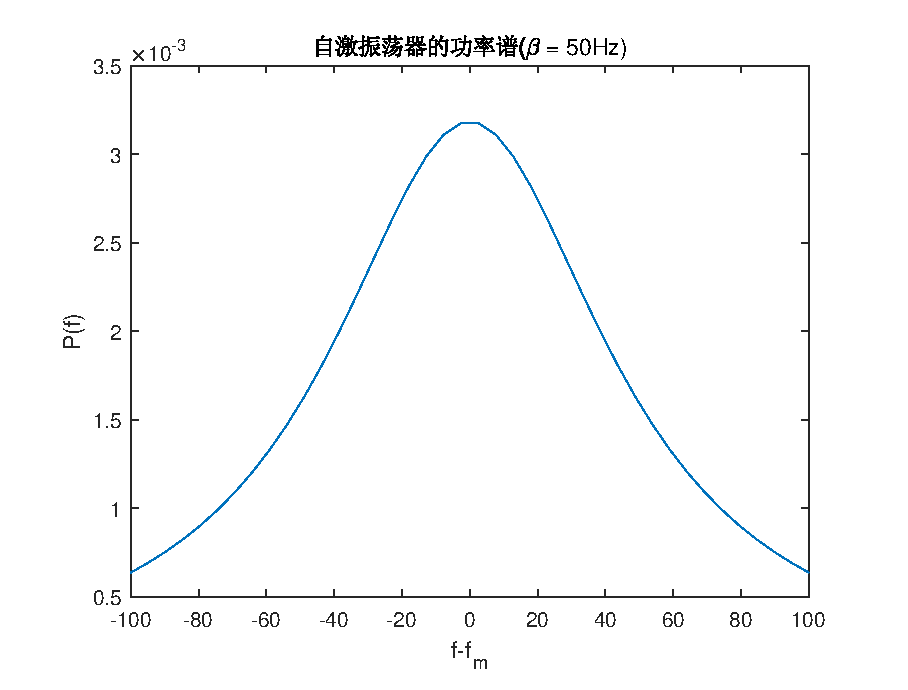
\includegraphics{images/PN.eps}
					}
					%\includegraphics[scale=1.0]{figurefile}
					$\quad$\caption{$\beta=50$Hz时的相位噪声的功率谱}
					\label{fig:campus}
				\end{figure}
			\end{column}%
			\hfill%
			\begin{column}<0->{.5\textwidth}
				\begin{itemize}
					\item 参数$c$表示相位噪声的波动率.
					\item 功率谱密度函数为$P(f) = \frac{c/2}{4{{\pi }^{2}}{{(f-{{f}_{m}})}^{2}}+{{\left( c/2 \right)}^{2}}}$
					\item 复数振荡器输出信号的3-dB带宽为$\beta = \frac{c}{4\pi}$ 
					\item 以$T_s$为时间间隔进行抽样后有$\phi[n+1]-\phi[n]\sim\mathcal{N}(0,cT_s)$
				\end{itemize}
			\end{column}%
		\end{columns}
	\end{frame}

	\begin{frame}{\textbf{小结}}
		\begin{block}{在发送端考虑的RF}
			\begin{itemize}
				\item I/Q不平衡系数:$\alpha_{I,tx}$与$\alpha_{Q,tx}$
				\item 相位的不匹配$\theta_{I,tx}$与$\theta_{Q,tx}$
				\item 相位的噪声过程$\phi_{tx}(t)$
			\end{itemize}
		\end{block}
	
		\begin{block}{在接收端考虑的RF}
		\begin{itemize}
			\item I/Q不平衡系数:$\alpha_{I,rx}$与$\alpha_{Q,rx}$
			\item 相位的不匹配$\theta_{I,rx}$与$\theta_{Q,rx}$
			\item 相位的噪声过程$\phi_{rx}(t)$
		\end{itemize}
		\end{block}
	\end{frame}
\section{自干扰的产生和消除过程}
    
    \frame{\sectionpage}
\begin{frame}{\textbf{多径信道与ALC}}
	\begin{columns}[T] % align columns
		\begin{column}<0->{.40\textwidth}
			\begin{figure}[thpb]
				\centering
				\resizebox{1\linewidth}{!}{
					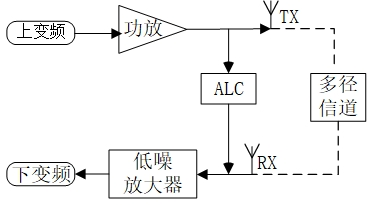
\includegraphics{images/alc.jpg}
				}
				%\includegraphics[scale=1.0]{figurefile}
				$\quad$\caption{多径信道与模拟域线性消除}
				\label{fig:campus}
			\end{figure}
		\end{column}%
		\hfill%
		\begin{column}<0->{.5\textwidth}
			\begin{itemize}
				\item 多径信道中传来的自干扰为$ax_p(t-\delta) + \sum_{c=1}^{L}a_cx_p(t-\delta_c)$
				\item 模拟域线性消除项为$\widehat{a}x_p(t-\widehat{\delta})$
				\item ALC消除结果是
				\begin{equation*}
					\begin{split}
						y_p(t) &= ax_p(t-\delta) - \widehat{a}x_p(t-\widehat{\delta}) \\
						&+ \sum_{c=1}^{L}a_cx_p(t-\delta_c)
					\end{split}
				\end{equation*}
				\item 其中$\forall c\in\{1,\cdots,L\},a_c\sim\mathcal{CN}(0,\sigma^2_{a,c})$
				\item $a\sim \mathcal{CN}(0,\sigma^2_{a})$
			\end{itemize}
		\end{column}%
	\end{columns}
\end{frame}

\begin{frame}
	\begin{block}{$y_p(t)$经过下变频的混频器和低通滤波器后得到}
		\begin{equation*}
			\begin{split}
			\tilde{y}(t) = &\mu_{rx}e^{-j\phi_{rx}(t)} \Big\{  ae^{-j\omega_m\delta}e^{j\phi_{tx}(t-\delta)}[\mu_{tx}x(t-\delta)+\nu_{tx}^{*}x^{*}(t-\delta)] \\
			&- \hat{a} e^{-j\omega_m\hat\delta}e^{j\phi_{tx}(t-\hat\delta)}[\mu_{tx}x(t-\hat\delta)+\nu_{tx}^{*}x^{*}(t-\hat\delta)] \\
			& + \sum_{c=1}^{L}a_ce^{-j\omega_m\delta_c}e^{j\phi_{tx}(t-\delta_c)}[\mu_{tx}x(t-\delta_c)+\nu_{tx}^{*}x^{*}(t-\delta_c)] \Big\}  \\
			&+ \nu_{rx}e^{j\phi_{rx}(t)} \Big\{  a^{*}e^{j\omega_m\delta}e^{-j\phi_{tx}(t-\delta)}[\mu_{tx}^{*}x^{*}(t-\delta)+\nu_{tx}x(t-\delta)] \\
			&- \hat{a}^{*} e^{j\omega_m\hat\delta}e^{-j\phi_{tx}(t-\hat\delta)}[\mu_{tx}^{*}x^{*}(t-\hat\delta)+\nu_{tx}x(t-\hat\delta)] \\
			& + \sum_{c=1}^{L}a_c^{*}e^{j\omega_m\delta_c}e^{-j\phi_{tx}(t-\delta_c)}[\mu_{tx}^{*}x^{*}(t-\delta_c)+\nu_{tx}x(t-\delta_c)]  \Big\}
			\end{split}
		\end{equation*}
	\end{block}
\end{frame}  

\begin{frame}
	\begin{block}{引入$s(t)=x(t-\delta) \approx x(t-\hat\delta),s_c(t)=x(t-\delta_c)$,
			并记$p(t) = e^{j[\phi_{tx}(t-\delta)-\phi_{rx}(t)]} $ 和 $\ p_c(t) = e^{j[\phi_{tx}(t-\delta_c)-\phi_{rx}(t)]}$化简得到}
		\begin{equation*}
		\begin{split}
		\tilde{y}(t)  \approx &\mu_{rx} \Big\{  ap(t)e^{-j\omega_m\delta}[\mu_{tx}s(t)+\nu^{*}_{tx}s^*(t)] \\
		&- \hat{a}p(t)e^{-j\omega_m\hat\delta}[\mu_{tx}s(t)+\nu^{*}_{tx}s^*(t)]  \\
		&+ \sum_{c=1}^{L}a_cp_c(t)e^{-j\omega\delta_c}[\mu_{tx}s_c(t)+\nu^{*}_{tx}s_c^*(t)] \Big\}  \\
		&+ \nu_{rx} \Big\{  a^*p^*(t)e^{j\omega_m\delta}[\mu_{tx}^*s^*(t)+\nu_{tx}s(t)] \\
		&- \hat{a}^*p^*(t)e^{j\omega_m\hat\delta}[\mu_{tx}^*s^*(t)+\nu_{tx}s(t)]  \\
		&+ \sum_{c=1}^{L}a_c^*p^*_c(t)e^{j\omega\delta_c}[\mu_{tx}^*s_c^*(t)+\nu_{tx}s_c(t)] \Big\}
		\end{split}
		\end{equation*}
	\end{block}
\end{frame}

\begin{frame}{抽样和FFT}
	\begin{block}{将$\tilde{y}(t)$经过抽样,再进行FFT}
		\begin{equation*}
			\begin{split}
			y_n &= \mu_{rx} \sum_{c=0}^{L}a_ce^{-j\omega_{m}(cT_s + \delta)+j[\phi_{tx}(nT_s-cT_s-\delta)-\phi_{rx}(nT_s)]} \{ \mu_{tx}s_{n-c}+\nu_{tx}^{*}s^{*}_{n-c} \} \\
			&+ \nu_{rx} \sum_{c=0}^{L}a_c^*e^{j\omega_{m}(cT_s + \delta)-j[\phi_{tx}(nT_s-cT_s-\delta)-\phi_{rx}(nT_s)]} \{ \mu_{tx}^*s^*_{n-c}+\nu_{tx}s_{n-c} \}
			\end{split}
		\end{equation*}
		\begin{equation*}
			\begin{split}
			Y_k &= \sum_{c=0}^{L}a_ce^{-j\omega_{m}(cT_s + \delta)} \big\{ (\mu_{rx}\mu_{tx}S_kW_N^{ck}+\mu_{rx}\nu_{tx}^*S^*_{N-k}W_N^{ck}) \bigotimes P^{(1)}_k  \big\} \\
			&+ \sum_{c=0}^{L}a_c^*e^{j\omega_{m}(cT_s + \delta)}  \big\{ (\nu_{rx}\mu_{tx}^*S^*_{N-k}W_N^{ck}+\nu_{rx}\nu_{tx}S_kW_N^{ck}) \bigotimes P^{(2)}_k  \big\}
			\end{split}
		\end{equation*}
	\end{block}
\end{frame}

\begin{frame}{数字自干扰消除前的自干扰功率是}
	\begin{equation*}
	\begin{split}
	\mathbb{E}|Y[k]|^2 &=\sum_{c=0}^{L}\sigma_{a,c}^2\sum_{l=0}^{N-1}(|\mu_{rx}\mu_{tx}|^2\mathcal{E}_{l}+|\mu_{rx}\nu_{tx}|^2\mathcal{E}_{N-l})\mathbb{E}\big| P^{(1)}[k-l]\big|^2\\
	&+ \sum_{c=0}^{L}\sigma_{a,c}^2\sum_{l=0}^{N-1}(|\nu_{rx}\mu_{tx}|^2\mathcal{E}_{N-l}+|\nu_{rx}\nu_{tx}|^2\mathcal{E}_{l}) \mathbb{E}\big|P^{(2)}[k-l]\big|^2
	\end{split}
	\end{equation*}
	
	其中$\mathbb{E}\big|P^{(i)}[k-l]\big|^2$和收发两端是共用同一个振荡器还是使用两个独立的振荡器有关  
	
\end{frame}

\begin{frame}
	\begin{block}{$\mathbb{E}\big|P^{(i)}[k-l]\big|^2,i=1,2$的理论计算结果}
		\begin{itemize}
			\item 收发两端是共用同一个振荡器\begin{equation*}
			\begin{split}
			\mathbb{E}\big|P^{(i)}[k]\big|^2 =\frac{1}{N^2}\bigg[ -N&+\sum_{n=0}^{c} 2(N-n)e^{-4\pi n\beta T_s}\cos \big(\frac{2\pi kn}{N} \big) \\
			&+e^{-4\pi\beta(cT_s+\delta)}\sum_{n=c+1}^{N-1}2(N-n)\cos\big(\frac{2\pi kn}{N} \big)\bigg].
			\end{split}
			\end{equation*}
			\item 收发两端使用两个独立的振荡器\begin{equation*}
			\mathbb{E}\big|P^{(i)}[k]\big|^2 = \frac{1}{N^2}\bigg[ -N+\sum_{n=0}^{N-1} 2(N-n)e^{-4\pi n\beta T_s}\cos \big(\frac{2\pi kn}{N} \big)\bigg].
			\end{equation*}
		\end{itemize}
	\end{block}
\end{frame}

\begin{frame}{数字域消除后的剩余自干扰功率$\mathbb{E}|U[k]|^2$}
	\begin{columns}[T] % align columns
		\begin{column}<0->{.40\textwidth}
			\begin{equation*}
			\begin{split}
			&\mathbb{E}|U[k]|^2 = \\
			&\sum_{c=0}^{L}\sigma_{a,c}^2\sum_{\substack{l=0 \\ l\neq k}}^{N-1}(|\mu_{rx}\mu_{tx}|^2\mathcal{E}_{l})\mathbb{E}\big| P^{(1)}_{k-l}\big|^2\\
			&+\sum_{c=0}^{L}\sigma_{a,c}^2\sum_{l=0}^{N-1}(|\mu_{rx}\nu_{tx}|^2\mathcal{E}_{N-l})\mathbb{E}\big| P^{(1)}_{k-l}\big|^2\\
			&+ \sum_{c=0}^{L}\sigma_{a,c}^2\sum_{l=0}^{N-1}(|\nu_{rx}\mu_{tx}|^2\mathcal{E}_{N-l}+|\nu_{rx}\nu_{tx}|^2\mathcal{E}_{l}) \mathbb{E}\big|P^{(2)}_{k-l}\big|^2 \\
			&+ |\mu_{rx}\mu_{tx}|^2\mathcal{E}_{k}\mathrm{var}[\widehat{a_c}]\mathbb{E}\big|P^{(1)}_{0}\big|^2.
			\end{split}
			\end{equation*}
		\end{column}%
		\hfill%
		\begin{column}<0->{.4\textwidth}
			它与以下几点有关
			\begin{itemize}
				\item 相位噪声的3-dB带宽;
				\item 多径信道功率;
				\item 模拟域消除和数字域消除水平;
				\item 多径延时;
				\item I/Q不平衡水平.
			\end{itemize}
		\end{column}%
	\end{columns}
\end{frame}

\section{仿真与分析}
    
    \frame{\sectionpage}
    
    \begin{frame}{仿真与分析}
    \begin{itemize}
    	\item OFDM系统的建立
    	\item 仅有相位噪声时
    	
    	\item 联合讨论相位噪声和I/Q不平衡
    \end{itemize}
    \end{frame}

	\begin{frame}
		\begin{block}{\textbf{基本思路}}
			\begin{itemize}
				\item 使用编辑距离矩阵将类似的消息归于一张连通图中。
				\item 使用固定值替换感兴趣的消息,如代码、email地址。
				\item 查找归一化距离小于阈值的消息,并确定聚类边界。
			\end{itemize}
		\end{block}
	
		\begin{block}{\textbf{基本思路}}
			\begin{itemize}
				\item 使用编辑距离矩阵将类似的消息归于一张连通图中。
				\item 使用固定值替换感兴趣的消息,如代码、email地址。
				\item 查找归一化距离小于阈值的消息,并确定聚类边界。
			\end{itemize}
		\end{block}
	\end{frame}
    
\section{大数定律与中心极限定理}
    
    \frame{\sectionpage}
    
     \begin{frame}{特征函数和概率极限定理}
    \begin{itemize}
    	\item 随机变量的收敛性
    	
    	$\quad$依分布收敛、依概率收敛、几乎处处收敛、$L^p$收敛
    	\item 概率母函数、特征函数
    	\item 大数定律
    	\item 中心极限定理
    \end{itemize}
\end{frame}

\begin{frame}{\textbf{概率母函数} Probability Generating Function}
		\begin{block}{\textbf{Def 1.1}$\quad$对一个只取非负整数值的离散型随机变量$X$}
		其母函数定义为\begin{equation}
			g(s) = \mathrm{E}(s^X) = \sum_{j=0}^\infty s^jP(X=j),s\in [-1,1].
		\end{equation}
	\end{block}
	概率母函数的引入为计算取非负整数值的随机变量的概率分布、数学期望和方差等带来了很多的方便.
	\begin{itemize}
		\item 这个定义的存在性是由于$|s^X|\leqslant 1$保证了所求数学期望的存在性;
		\item 此处约定$0^0 = 1$.
	\end{itemize}

\end{frame}

\begin{frame}{\textbf{概率母函数} Probability Generating Function}
\begin{block}{\textbf{Thm 1.1}假设$g(s)$是$X$的母函数,则有}
	\begin{itemize}
		\item $P(X=k) = \frac{1}{k!}g^{(k)}(0),k=0,1,\cdots$;
		\item $\mathrm{E}X = g'(1)$;
		\item 如果$\mathrm{E}X<\infty$,则$\mathrm{var}(X) = g''(1)+g'(1)-(g'(1))^2$;
		\item 如果$X_1,X_2,\cdots,X_n$相互独立,$g_j(s) = \mathrm{E}s^{X_j}$是$X_j$的母函数,则$Y = X_1+X_2+\cdots+X_n$有母函数
		\begin{equation}
			g_Y(s) = g_1(s)g_2(s)\cdots g_n(s),s\in [-1,1].
		\end{equation}
	\end{itemize}	
\end{block}
\end{frame}

\begin{frame}
	\textbf{证明}$\quad$
	
	(1)\begin{equation}
		\begin{split}
			\frac{1}{k!}g^{(k)}(0) &= \frac{1}{k!}g^{(k)}(s)\bigg|_{s=0} \\
			&= \frac{1}{k!}\sum_{j=k}^\infty\frac{\mathrm{d}^k}{\mathrm{d}s^k}(s^j)P(X=j)\bigg|_{s=0} \\
			&= P(X=k).
		\end{split}
	\end{equation}
	
	(2)由$g'(1) = \sum\limits_{j=0}^\infty jP(X=j) = \mathrm{E}X$得到.
	
	(3)由\begin{equation}
		g''(1) = \sum_{j=0}^\infty j(j-1)P(X=j) = \mathrm{E}[X(X-1)]
	\end{equation}
\end{frame}

\begin{frame}
	得到\begin{equation}
		g''(1)+g'(1) - (g'(1))^2 = \mathrm{E}[X(X-1)] + \mathrm{E}X - (\mathrm{E}X)^2 = \mathrm{var}(X).
	\end{equation}
	
	(4)由于$X_1,X_2,\cdots,X_n$相互独立,所以随机变量$s^{X_1},s^{X_2},\cdots,s^{X_n}$相互独立.
	
	又由于$\left|s^{X_1+X_2+\cdots+X_n}\right|\leqslant 1$,所以可以使用Fubini定理,因此,
	\begin{equation}
		g_Y(s) = \mathrm{E}s^{X_1+X_2+\cdots+X_n} = \mathrm{E}s^{X_1}\cdots\mathrm{E}s^{X_n} = g_1(s)g_2(s)\cdots g_n(s)
	\end{equation}
	
	Rmk:结论(1)说明了对于只取非负整数值的随机变量,\alert{母函数和概率分布相互唯一决定}(determine).
\end{frame}

\begin{frame}
	\textbf{例}$\quad$二项分布$\mathcal{B}(n,p)$的母函数是
	\begin{equation}
		g(s) = \sum_{j=0}^ns^j\binom{n}{j}p^jq^{n-j} = (q+sp)^n.
	\end{equation}
	此外,设$X_1,X_2,\cdots,X_m$相互独立,$X_j\sim \mathcal{B}(n_j,p)$,则
	\begin{equation}
		Y = X_1+X_2+\cdots+X_m
	\end{equation}
	有母函数
	\begin{equation}
		\begin{split}
			g_Y(s) &= (q+sp)^{n_1}\cdots(q+sp)^{n_m} \\
			&= (q+sp)^n,n = n_1+\cdots+n_m.
		\end{split}
	\end{equation}
	说明$Y\sim\mathcal{B}(n_1+\cdots+n_m,p)$.
\end{frame}

\begin{frame}
	\textbf{例}$\quad$泊松分布$\mathcal{P}(\lambda)$的母函数是
	\begin{equation}
		g(s) = \sum_{k=0}^\infty s^k\frac{\lambda^k}{k!}e^{-\lambda} = e^{\lambda (s-1)}.
	\end{equation}
	此外,设$X_1,X_2,\cdots,X_m$相互独立,$X_j\sim \mathcal{P}(\lambda_j)$,则
	\begin{equation}
	Y = X_1+X_2+\cdots+X_m
	\end{equation}
	有母函数
	\begin{equation}
	\begin{split}
	g_Y(s) &= e^{\lambda_1 (s-1)}\cdots e^{\lambda_m (s-1)} \\
	&= e^{\lambda (s-1)},\lambda = \lambda_1+\cdots+\lambda_m.
	\end{split}
	\end{equation}
	说明$Y\sim\mathcal{P}(\lambda_1+\cdots+\lambda_m)$.
\end{frame}

\begin{frame}
	\textbf{例}$\quad$$X$服从几何分布$\mathcal{G}(p)$,它有母函数\begin{equation}
		g(s) = \sum_{j=1}^\infty s^jpq^{j-1} = \frac{sp}{1-sq}.
	\end{equation}
	此外,设$X_1,X_2,\cdots,X_m$相互独立,都服从相同的几何分布$\mathcal{G}(p)$,则
	$Y = X_1+X_2+\cdots+X_m$有母函数
	\begin{equation}
		g_Y(s) = \left(\frac{sp}{1-sq}\right)^m.
	\end{equation}
	将上式的右边进行Taylor展开,得到
	\begin{equation}
	\begin{split}
		g_Y(s) &= (sp)^m\sum_{j=0}^\infty \frac{m(m+1)\cdots(m+j-1)}{j!}(sq)^j \\
		&= (sp)^m\sum_{j=0}^\infty\binom{m+j-1}{m-1}(sq)^j \\
		&= \sum_{k=m}^\infty\binom{k-1}{m-1}p^mq^{k-m}s^k
	\end{split}
	\end{equation}
\end{frame}

\begin{frame}
	于是得到Pascal(帕斯卡)分布
	\begin{equation}
		P(Y=k) = \binom{k-1}{m-1}p^mq^{k-m},k=m,m+1,\cdots.
	\end{equation}
	回忆在前面的讨论中,$Y$是第$m$次击中目标时的射击总次数.
	\\ \hspace*{\fill} \\%空行
	\textbf{练习}$\quad$掷三枚骰子,求点数之和是9的概率.
	
	\textbf{解}$\quad$用$X_i$表示第$i$颗骰子的点数,$i=1,2,3$,则$Y=X_1+X_2+X_3$是三颗骰子的总点数.由
	\begin{equation}
		g(s) = \mathrm{E}s^{X_1} = \frac{1}{6}(s+s^2+\cdots+s^6) = \frac{1}{6}\frac{s(1-s^6)}{1-s}.
	\end{equation}
\end{frame}

\begin{frame}
	得到$Y$的母函数\begin{equation}
	\begin{split}
		g_Y(s) &= g^3(s) = \frac{s^3(1-s^6)^3}{6^3(1-s)^3} \\
		&= \frac{1}{6^3}s^3(1-3s^6+3s^{12}-s^{18})\sum_{k=0}^\infty\binom{k+2}{2}s^k.
	\end{split}
	\end{equation}
	可以算出$s^9$的系数是
	\begin{equation}
		P(Y=9) = \frac{1}{6^3}\left(\binom{6+2}{2}-3 \right) = \frac{25}{216}.
	\end{equation}
	\textbf{练习}$\quad$设$p=1-q\in(0,1)$,验证对数正态分布\begin{equation}
		P(X=k) = -\frac{q^k}{k\ln p},k=1,2,\cdots
	\end{equation}
	的母函数和数学期望分别是\begin{equation}
		\frac{\ln(1-qs)}{\ln p}\text{和}\frac{-q}{p\ln p}.
	\end{equation}
\end{frame}

\begin{frame}{\textbf{特征函数} Characteristic Function}
\begin{block}{\textbf{Def 2.1}如果$\xi,\eta$是随机变量,$i=\sqrt{-1}$,则称}
	\begin{equation}
		Z=\xi + i\eta
	\end{equation}
	是复值随机变量.如果$\mathrm{E}\xi,\mathrm{E}\eta$都存在,则$Z$的数学期望为
	\begin{equation}
		\mathrm{E}Z = \mathrm{E}\xi + i\mathrm{E}\eta.
	\end{equation}
\end{block}
没有特殊声明时,以下讨论的随机变量还都是实值的.
\end{frame}

\begin{frame}{\textbf{特征函数} Characteristic Function}
\begin{block}{\textbf{Def 2.2}对随机变量$X$,}
	由于$\sin(tX),\cos(tX)$的数学期望都存在,于是可以定义\begin{equation}
	\phi(t) \stackrel{\text{def}}{=}\mathrm{E}e^{itX} = \mathrm{E}\cos(tX) + i\mathrm{E}\sin(tX),t\in\mathbb{R}
	\end{equation}
	称上式定义的$\phi(t)$为$X$的\alert{特征函数}.
\end{block}
\begin{itemize}
	\item 当$X$为离散型时: $P(X=x_k) = p_k,k=1,2,\cdots$,
	\begin{equation}
		\phi(t) = \sum_{k}e^{itx_k}p_k.
	\end{equation}
	\item 当$X$为连续型时:$X$有密度$f(x)$
	\begin{equation}
		\phi(t) = \int_{-\infty }^\infty e^{itx}f(x)\mathrm{d}x.
	\end{equation}
\end{itemize}
\end{frame}

\begin{frame}
	\textbf{Rmk1}:不同的数学群体对于\alert{Fourier变换}的定义会略有不同.
	\begin{itemize}
		\item 不少的文献把$F$的Fourier-Stieltjes变换定义成
			\begin{equation}
				\frac{1}{(2\pi)^n}\int_{\mathbb{R}^n}\exp(-i\bm{\xi}\cdot\bm{y})\mathrm{d}F(\bm{y}).
			\end{equation}
		\item 有些文献则把$F$的Fourier-Stieltjes变换定义成
			\begin{equation}
				\int_{\mathbb{R}^n}\exp(i\bm{t}\cdot\bm{y})\mathrm{d}F(\bm{y}).
			\end{equation}
	\end{itemize}
	概率论的文献中通常使用后一个定义,且把Fourier变换改称为\textbf{特征函数}.这样的差异仅仅是Fourier变换及逆变换的公式的形式上的,并不会给数学理论带来重大的改变.
	
	\textbf{Rmk2}:在概率论以外的其它的数学分支中,还有一些不同含义的函数也被称为"特征函数",切勿与此混淆,一个是线性算子的特征函数(本征函数),另一个是集合的特征函数(指示函数、示性函数)
\end{frame}

\begin{frame}
	\textbf{Rmk3}:对每个分布函数$F$,可以在$\mathbb{R}$上引进唯一的一个Borel测度$\mu$,使得任何满足条件的$a\leqslant b$的实数$a$和$b$,都有以下等式:
	\begin{equation}
		\mu((a,b]) = F(b) - F(a).
	\end{equation}
	这个Borel测度$\mu$时常记作$\mu = \mathrm{d}F$.
	
	特征函数也常记作\begin{equation}
		\phi(t) = \int_{-\infty}^\infty e^{itx}\mu(\mathrm{d}x).
	\end{equation}
	多元的情况也有类似的公式.
\end{frame}

\begin{frame}
	\textbf{例}$\quad$(Coin Flips)设$P(X=1) = P(X=-1) = 1/2$,则
	\begin{equation}
		\mathrm{E}e^{itX} = (e^{it}+e^{-it})/2 = \cos t.
	\end{equation}
	
	\textbf{例}$\quad$(Poisson分布)设$P(X=k) = e^{-\lambda}\lambda^k/k!$,for $k = 0,1,2,\cdots$
	\begin{equation}
		\mathrm{E}e^{itX} = \sum_{k=0}^\infty e^{-\lambda}\frac{\lambda^k e^{itk}}{k!} = \exp(\lambda (e^{it}-1)).
	\end{equation}
	
	\textbf{例}$\quad$(二项(Binomial)分布)设$X\sim \mathcal{B}(n,p)$
	\begin{equation}
	\begin{split}
		\mathrm{E}e^{itX} &= \sum_{k=0}^n\binom{n}{k}p^kq^{n-k}e^{itk} \\
		&=\sum_{k=0}^n\binom{n}{k}(pe^{it})^kq^{n-k} \\
		&=(pe^{it}+q)^n.
		\end{split}
	\end{equation}
	
\end{frame}

\begin{frame}
	\textbf{例}$\quad$(几何分布)设$X\sim\mathcal{G}(p),P(X=k)=pq^{k-1},k=1,2,\cdots.$
	\begin{equation}
	\begin{split}
	\mathrm{E}e^{itX} &= \sum_{k=1}^\infty pq^{k-1}e^{itk} \\
	&=\sum_{k=1}^\infty pe^{it}(qe^{it})^{k-1}\\
	&=\frac{pe^{it}}{1-qe^{it}}.
	\end{split}
	\end{equation}
	
	\textbf{例}$\quad$(负二项分布)设$P(X=k)=\binom{k+r-1}{r-1}q^kp^r,k=0,1,\cdots$,其中$p+q=1,pq>0.$
	\begin{equation}
	\begin{split}
	\mathrm{E}e^{itX} &= \sum_{k=0}^\infty \binom{k+r-1}{r-1}q^kp^re^{itk} \\
	&=\left(\frac{p}{1-qe^{it}}\right)^r.
	\end{split}
	\end{equation}
\end{frame}


\begin{frame}
	\textbf{例}$\quad$Uniform distribution on $(a,b)$
	
	解: 根据
	\begin{equation}
		\int_{a}^{b}e^{\lambda x}\mathrm{d}x = (e^{\lambda b}-e^{\lambda a})/\lambda,\forall \lambda\in\mathbb{C}
	\end{equation}	
	得到
	\begin{equation}
	\begin{split}
	\phi(t) &= \int_{-\infty}^\infty e^{itx}f(x)\mathrm{d}x \\
	&=\int_{a}^b e^{itx}/(b-a)\mathrm{d}x  \\
	&= \frac{e^{itb}-e^{ita}}{it(b-a)}.
	\end{split}
	\end{equation}
	Special Case:$(a,b)=(-c,c)$,
	
	Ch.f. $\phi(t) = \frac{\sin(ct)}{ct}$.
	
\end{frame}

\begin{frame}
	\textbf{例}$\quad$(Exponential distribution)设$X\sim\mathcal{E}(\lambda)$.
	
	Density:\begin{equation}
		f(x) =\lambda e^{-\lambda x}\bm{1}_{(x>0)}.
	\end{equation}

	Ch.f.:\begin{equation}
		\phi(t) = \int_{0}^\infty e^{itx}\lambda e^{-\lambda x}\mathrm{d}x = \frac{\lambda e^{(it-\lambda)x}}{it-\lambda}\bigg|^{+\infty}_0 = \frac{\lambda}{\lambda - it}.
	\end{equation}
	since:$|e^{(it-\lambda)x}| = e^{-\lambda x}\to 0$, as $x\to+\infty$

\end{frame}

\begin{frame}
\textbf{例}$\quad$(标准正态分布)设$X\sim\mathcal{N}(0,1)$.

Ch.f.:\begin{equation}
\phi(t) = \int_{\mathbb{R}}e^{itx}\frac{1}{\sqrt{2\pi}}e^{-x^2/2}\mathrm{d}x.
\end{equation}
形式上的计算(cheat):
\begin{equation}
	\int_{\mathbb{R}}e^{itx}\frac{1}{\sqrt{2\pi}}e^{-x^2/2}\mathrm{d}x = 
	e^{-t^2/2}\int_{\mathbb{R}}\frac{1}{\sqrt{2\pi}}e^{-(x-it)^2/2}\mathrm{d}x = e^{-t^2/2}.
\end{equation}
数学上的证明:
\begin{equation}
	\begin{split}
		\phi(t) &= \int_{\mathbb{R}}e^{itx}\frac{1}{\sqrt{2\pi}}e^{-x^2/2}\mathrm{d}x\\
		&= \int_{\mathbb{R}}\cos(tx)\frac{1}{\sqrt{2\pi}}e^{-x^2/2}\mathrm{d}x.
	\end{split}
\end{equation}
since: $\sin(tx)$:odd.
\end{frame}

\begin{frame}
	\begin{equation}
	\begin{split}
	\phi'(t) &= \int_{\mathbb{R}}-x\sin(tx)\frac{1}{\sqrt{2\pi}}e^{-x^2/2}\mathrm{d}x\\
	&= -\int_{\mathbb{R}}t\cos(tx)\frac{1}{\sqrt{2\pi}}e^{-x^2/2}\mathrm{d}x\text{(分部积分)}\\
	&= -t\phi(t)
	\end{split}
	\end{equation}
	\begin{equation*}
		\phi'(t) = -t\phi(t)\xRightarrow[]{implies} \frac{\mathrm{d}}{\mathrm{d}t}\{\phi(t)\exp(t^2/2)\} = 0.
	\end{equation*}
	因此,$\phi(t)\exp(t^2/2) = \phi(0) = 1.$证毕.
	评:此例中用到了著名的\textbf{Fresnel积分},这两个积分是Fresnel在研究光学中首次碰到的.
\end{frame}

\begin{frame}
	\textbf{例}$\quad$($\Gamma(\alpha,\beta)$分布)设$X$有密度
	\begin{equation}
		f(x) = \frac{\beta^\alpha}{\Gamma(\alpha)}x^{\alpha-1}e^{-\beta x}\bm{1}_{(x>0)}.
	\end{equation}
	则特征函数为:
	\begin{equation}
		\begin{split}
			\phi(t) &= \int_{0}^\infty  \frac{\beta^\alpha}{\Gamma(\alpha)}x^{\alpha-1}e^{-\beta x}e^{itx}\mathrm{d}x \\
			&=  \frac{\beta^\alpha}{(\beta-it)^\alpha \Gamma(\alpha)}\int_{0}^\infty ((\beta-it)x)^\alpha e^{(it-\beta)x}\frac{\mathrm{d}x}{x} \\
			&= \frac{\beta^\alpha}{(\beta-it)^\alpha}.(\text{形式上})
		\end{split}
	\end{equation}
	Rmk:数学上可以通过复变函数的相关知识对上式进行严格的证明(略).
\end{frame}


\begin{frame}{\textbf{特征函数} Characteristic Function}
	特征函数的最重要的性质之一是如下的逆转公式(下面的证明不要求)
	\begin{block}{\textbf{Thm 2.1}(逆转公式)设$\phi(t)$是$X$的特征函数,$F(x)$是$X$的分布函数,则}
		\begin{equation}
			\overline{F}(b)-\overline{F}(a) = \frac{1}{2\pi}\lim_{T\to\infty}\int_{-T}^{T}\frac{e^{-itb}-e^{-ita}}{-it}\phi(t)\mathrm{d}t.
		\end{equation}
		\begin{itemize}
			\item 其中$\overline{F}(x) = \frac{F(x^+)+F(x^-)}{2},\forall x\in \mathbb{R}$
			\item $t=0$时,$\frac{e^{-itb}-e^{-ita}}{-it}$定义成$b-a$.
		\end{itemize}
	\end{block}
\end{frame}

\begin{frame}
	证明: 不妨设$a<b$,由于\begin{equation}
		\begin{split}
			\left|\frac{e^{-itb}-e^{-ita}}{-it} \right| &= \left|\int_{a}^{b}e^{-itx}\mathrm{d}x\right| \\
			 &\leqslant \int_{a}^{b}\left|e^{-itx}\right|\mathrm{d}x = b-a.
		\end{split}
		\end{equation}
		所以可以应用Fubini定理得到:
		\begin{equation}
		\begin{split}
			I_T &\stackrel{\text{def}}{=}\frac{1}{2\pi}\int_{-T}^{T}\frac{e^{-itb}-e^{-ita}}{-it}\phi(t)\mathrm{d}t \\
			&= \frac{1}{2\pi}\int_{-T}^{T}\frac{e^{-itb}-e^{-ita}}{-it}\int_{\mathbb{R}}e^{itx}\mathrm{d}F(x)\mathrm{d}t \\
			&=\frac{1}{2\pi}\int_{\mathbb{R}}\int_{-T}^{T}\frac{e^{it(x-b)}-e^{it(x-a)}}{-it}\mathrm{d}t\mathrm{d}F(x)
		\end{split}
		\end{equation}
\end{frame}

\begin{frame}
	根据奇偶性,将上式化简为
	\begin{equation}
		I_T=\frac{1}{\pi}\int_{\mathbb{R}}\int_{0}^{T}\frac{\sin(t(x-b))-\sin(t(x-a))}{-t}\mathrm{d}t\mathrm{d}F(x)
	\end{equation}
	记\begin{equation}
		J_T=\int_{0}^{T}\frac{\sin(t(x-b))-\sin(t(x-a))}{-t}\mathrm{d}t.
	\end{equation}
	根据\begin{equation}
		\int_{0}^{T}\frac{\sin(\alpha t)}{t}\mathrm{d}t = \int_{t=0}^{T}\frac{\sin(\alpha t)}{\alpha t}\mathrm{d}(\alpha t).
	\end{equation}
	回忆数学分析的结论:
	\begin{equation}
		\lim_{T\to\infty}\int_{0}^T\frac{\sin t}{t}\mathrm{d}t = \frac{\pi}{2}.
	\end{equation}
\end{frame}

\begin{frame}
	由此便得到:\begin{equation}
		\lim_{T\to\infty}J_T = 	\left\{
		\begin{aligned}
		&0, x<a\ or\ x>b \\
		&\frac{\pi}{2},x=a\ or\ x=b \\
		&\pi, a<x<b
		\end{aligned}
		\right.
	\end{equation}
	即\begin{equation}
		\lim_{T\to\infty}J_T = \frac{\pi}{2}[\bm{1}_{(a\leqslant x<b)}+\bm{1}_{(a<x\leqslant b)}].
	\end{equation}
	由Lebesgue有界收敛定理,\begin{equation}
	\begin{split}
		\lim_{T\to\infty}I_T &= \frac{1}{\pi}\int_{\mathbb{R}}\lim_{T\to\infty}J_T\mathrm{d}F(x) \\
		&= \frac{1}{\pi}\int_{\mathbb{R}}\frac{\pi}{2}[\bm{1}_{(a\leqslant x<b)}+\bm{1}_{(a<x\leqslant b)}]\mathrm{d}F(x) \\
		&= \frac{1}{2}[F(b^-)-F(a^-)]+\frac{1}{2}[F(b)-F(a)] \\
		&= \overline{F}(b)-\overline{F}(a).
	\end{split}		
	\end{equation}
	证毕.
\end{frame}

\begin{frame}
	\textbf{Rmk1}:这个定理也可以写作:
	\begin{equation}
	\mu((a,b)) + \frac{1}{2}\mu(\{a,b\}) = \frac{1}{2\pi}\lim_{T\to\infty}\int_{-T}^{T}\frac{e^{-itb}-e^{-ita}}{-it}\phi(t)\mathrm{d}t.
	\end{equation}
	
	\textbf{Rmk2}:若$a$和$b$是分布函数$F(x)$的连续点,我们便得到
	\begin{equation}
	F(b)-F(a) = \frac{1}{2\pi}\lim_{T\to\infty}\int_{-T}^{T}\frac{e^{-itb}-e^{-ita}}{-it}\phi(t)\mathrm{d}t.
	\end{equation}
\end{frame}

\begin{frame}
\begin{block}{\textbf{Thm $2.1^*$}(逆转公式)设$\phi(t)$是$X$的特征函数,$F(x)$是$X$的分布函数,则}
	如果\begin{equation}
	\int_{-\infty}^\infty |\phi(t)|\mathrm{d}t<\infty
	\end{equation},
	则$X$还有有界且连续的概率密度函数$f(x)$,使得累积概率测度分布函数$F(x)$可以表示成
	\begin{equation}
	F(x) = \int_{-\infty}^x f(y)\mathrm{d}y.
	\end{equation}
	进一步,概率密度$f(x)$可以通过特征函数$\phi(t)$用以下的反演公式表示:
	\begin{equation}
	f(x) = \frac{1}{2\pi}\int_{-\infty}^\infty e^{-itx}\phi(t)\mathrm{d}t.
	\end{equation}
\end{block}
\end{frame}

\begin{frame}
	证明:由于\begin{equation}
		\left|\frac{e^{-itb}-e^{-ita}}{-it} \right|\leqslant |b-a|.
	\end{equation}
	所以得到:
	\begin{equation}
		\begin{split}
			\mu((a,b)) + \frac{1}{2}\mu(\{a,b\}) &= \frac{1}{2\pi}\lim_{T\to\infty}\int_{-T}^{T}\frac{e^{-itb}-e^{-ita}}{-it}\phi(t)\mathrm{d}t \\
			&\leqslant \frac{b-a}{2\pi}\lim_{T\to\infty}\int_{-T}^{T}|\phi(t)|\mathrm{d}t
		\end{split}
	\end{equation}
	这说明$\mu$没有点测度.进一步,运用Fubini-Tonelli定理知道:
	\begin{equation}
		\begin{split}
			\mu((x,x+h)) &= \frac{1}{2\pi}\lim_{T\to\infty}\int_{-T}^{T}\frac{e^{-it(x+h)}-e^{-itx}}{-it}\phi(t)\mathrm{d}t \\
			&= \frac{1}{2\pi}\int_{-\infty}^{\infty}\left(\int_{x}^{x+h}e^{-ity}\mathrm{d}y\right)\phi(t)\mathrm{d}t \\
			&= \lim_{T\to\infty} \int_{x}^{x+h}\left(\frac{1}{2\pi}\int_{-\infty}^{\infty}e^{-ity}\phi(t)\mathrm{d}t \right)\mathrm{d}y
		\end{split}
	\end{equation}
\end{frame}

\begin{frame}
	这说明,$\mu$有密度函数\begin{equation}
		f(y) = \frac{1}{2\pi}\int_{-\infty}^{\infty}e^{-ity}\phi(t)\mathrm{d}t
	\end{equation}
	再根据控制收敛定理知道$f(x)$连续.
	\\ \hspace*{\fill} \\%空行
	\alert{Corollary}:概率测度分布函数$F$被它的特征函数$\phi$唯一确定.
	
	这就在理论上保证了:为了刻画随机变量,用概率测度分布函数的特征函数替代概率测度分布函数是不会丢失信息的.
\end{frame}

\begin{frame}
	\begin{block}{\textbf{Thm 2.2}任意的一个特征函数$\phi(t)$有如下性质}
	\begin{itemize}
		\item $\phi(0) = 1$
		\item $\phi(-t) = \overline{\phi(t)}$
		\item $|\phi(t)|=|\mathrm{E}e^{itX}|\leqslant \mathrm|e^{itX}| = 1$
		\item $|\phi(t+h)-\phi(t)|\leqslant \mathrm{E}|e^{ihX}-1|$,因此$\phi(t)$在$\mathbb{R}$上一致连续
		\item $\mathrm{E}e^{it(aX+b)} = e^{itb}\phi(at)$
	\end{itemize}
	
	\end{block}
\end{frame}



\section*{许宝騄的介绍}
\begin{frame}
	\begin{columns}[T] % align columns
		\begin{column}<0->{.40\textwidth}
			\begin{figure}[thpb]
				\centering
				\resizebox{1\linewidth}{!}{
					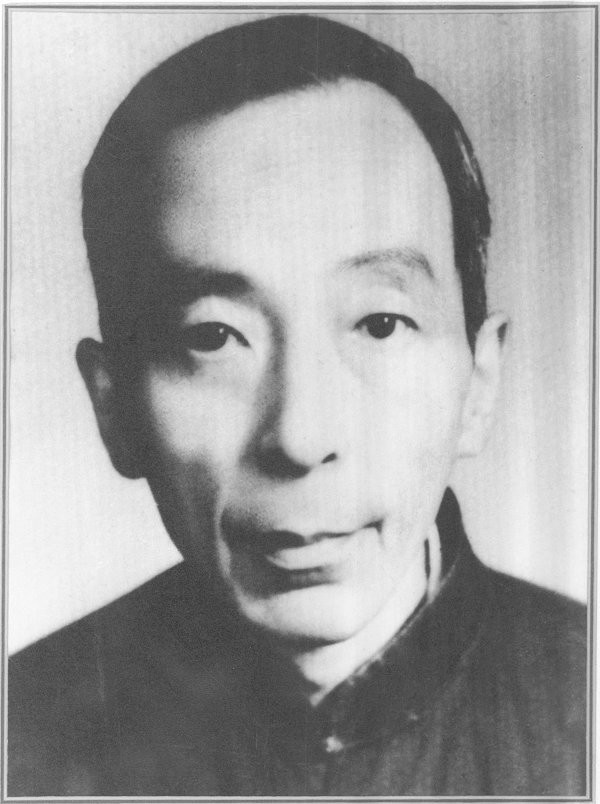
\includegraphics{images/PaoluXu.jpg}
				}
				%\includegraphics[scale=1.0]{figurefile}
				\caption{许宝騄}
				\label{fig:campus}
			\end{figure}
		\end{column}%
		\hfill%
		\begin{column}<0->{.6\textwidth}
			到现在,概率统计课已经进行了一半,我们在这里介绍一下我国非常著名的概率统计学家——许宝騄先生.应当说,他是我们国家概率统计事业的奠基人.
			
			\textbf{A、出身钱塘许氏}
			
			许宝騄(1910—1970年),字闲若,祖籍浙江杭州,1910年9月1日生于北京,因此小名京生。
			
			许宝騄在中国开创了概率论、数理统计的教学与研究工作。在奈曼-皮尔逊理论、参数估计理论、多元分析、极限理论等方面取得卓越成就,是多元统计分析学科的开拓者之一。其研究成果推动了概率论与数理统计的发展。 至今“许方法”(多元分析统计学家谢菲H.Scheffe称之为“数学严密性的范本”)仍被认为是解决检验问题的最实用方法。
		\end{column}%
	\end{columns}
	
\end{frame}

\begin{frame}
	$\quad$许宝騄是20世纪最富创造性的统计学家之一,也正是许宝騄拉开了中国概率论与数理统计学科研究的帷幕,他被公认为在数理统计和概率论方面第一个具有国际声望的中国数学家。《中国大百科全书 数学》称赞说:“许宝騄是中国早期从事数理统计学和概率论研究并达到世界先进水平的一位杰出学者。” 1983年,德国施普林格出版社刊印了《许宝騄全集》(Pao-Lu Hsu Collected Papers)由斯普林格(Springer-Verlag)出版社刊印,全集是由钟开莱主编的,共收集了已发表的、未被发表的论文40篇。书评中有这样一句话:
	
	“许宝騄被公认为在数理统计和概率论方面第一个具有国际声望的中国数学家”。
	
	许宝騄的像片悬挂在斯坦福大学统计系的走廊上,与世界著名的统计学家并列。
	
	$\quad$许宝騄是二十世纪和华罗庚、陈省身齐名的中国数学家,中央研究院第一届当选的5名数学所院士之一(注:另外四位首届数学院士是姜立夫、陈省身、华罗庚、苏步青)。当然由于各种原因的结果,他并不为国人所知。
\end{frame}

\begin{frame}
	$\quad$许先生出身于杭州的名门望族。据许氏家谱记载,杭州许氏本姓沈,始祖是富阳的沈显荣,1536年他在北京经商病故,遗有两子由杭州的表姑夫许魁带回杭州抚养,改姓许,入籍杭州。其中尤以横河桥支系的“积厚轩”堂兴旺。 
	
	$\quad$乾隆三年许家出了第一位举人许钺,之后钱塘许姓一族显宦至多,嘉庆、道光、同治间最盛。许氏十世祖许学范为乾隆三十七年(1772年)进士。许学范生得八个儿子,按照“学乃身之宝、儒以道得民”的行辈排下来,这八个儿子便被时人称人钱塘“八乃”,其中乃济、乃普、乃钊三子为进士,其余四子也皆中举人,皇帝给许家赐匾“七子登科”,意为许家府上出现过七位有才学的人。当时的学者、书法家梁同书曾写对联“世间数百年旧家,无非积德;天下第一件好事,还是读书”赠与许学范。
	
	$\quad$到光绪二十九年,共出了34位贡生、举人,其中9人中进士。许氏共有140多人次出任清代的大小官员,除江西省没有外,分布全国各省,名震朝野。老杭州都知道以前文武官员路过横河桥时,“文官下轿,武官下马”。就是因为许家有许多大官。
\end{frame}

\begin{frame}
	$\quad$许乃济(1777年—1839年),字叔舟,号青士,为嘉庆十四年(1814年)进士。选庶吉士,授编修。嘉庆二十五年(1825年)任山东道监察御史。道光三年(1823年)任兵科给事中。道光五年(1825年)任广东肇罗道,七年(1827年)改广东督粮道,道光九年(1829年)改高廉道。道光十三年(1833年)任光禄寺少卿,官至太常寺少卿。
	
	$\quad$许乃普(1787年—1866年),字贞锡,号滇生嘉庆二十五年(1820年)殿试高居一甲第二名(榜眼),赐进士及第,授翰林院编修。官至吏部尚书。同治五年(1866年)卒,谥文恪。工书,法二王,与祁寯藻、陈孚恩、赵光并称四书家。许乃普子彭寿为道光二十七年(1847年)丁未科会元,殿试位列二甲第一名(传胪)。选翰林院庶吉士。散馆授编修。官至内阁学士。
	
	$\quad$许乃赓为嘉庆二十二年(1817年)丁丑科二甲进士。改庶吉士,散馆授编修。历官右庶子。
\end{frame}

\begin{frame}
	$\quad$许宝騄的曾祖许乃钊(1799年-1878年)行七,字贞恒,号信臣,又号恂普,为道光十五年(1835年)殿试二甲、朝考一等第十名,授编修。之后历任国史馆总纂官,河南、广东学政,内阁学士兼礼部侍郎衔,江南大营帮办。咸丰三年(1853年),出任江苏巡抚,镇压上海小刀会起义,次年因无功被革职。咸丰七年(1857年),以三品顶戴帮办江南军务,咸丰八年(1858年),迁光禄寺卿。咸丰十年(1860年),太平军破江南大营,攻克苏州、常州,再次被革职。不久引疾回乡。光绪四年(1878年)卒。
	
	$\quad$许乃钊的子辈许祐身是许宝騄的祖父,累官至苏州知府。许宝騄父亲许引之从清朝末年至北洋政府时期一直担任中层官员,曾任清朝两浙盐运使。母亲程时嘉,江西新建人。
\end{frame}

\begin{frame}
	$\quad$许家为官当中有两人与慈禧60大寿和死亡有关。
	
	$\quad$许庚身(1825年-1893年),字星叔,号吉珊,崇尚天文、算术、舆地诸学。咸丰二年举人,考取内阁中书。同治元年,以在任官员的身份中进士,任内阁侍读。许庚身在军机处任职近三十年,曾参与策划对太平军和捻军的军事行动。同治十二年,任光禄寺卿。光绪五年,升任礼部侍郎,后分别任户部侍郎和刑部侍郎。中法战争爆发,许以刑部侍郎身份任军机大臣,兼总理各国事务衙门大臣,坚持以“驭夷无上策,可羁縻,不可迁就”的态度对待法国。十四年,升兵部尚书。
	
	$\quad$许庚身曾奉命总办慈禧60大寿,但是在寿前去世,清廷晋赠太子太保,谥恭慎。
	
\end{frame}

\begin{frame}
	$\quad$许宝蘅,光绪二十七年举人。他任军机章京时,记了许多日记,成为研究清末衰亡的重要史料。在光绪、慈禧死亡时,他记载了他忙碌的一天。早上五时,他至西苑门吉祥桥时,知道光绪于昨天酉时死了。进内宫后知道,昨天已颁发遗诏,传位于醇亲王之子,由摄政王监国。等到其他大官到场后,由他拟旨尊慈禧皇太后为太皇太后,皇后为皇太后。然后是拟各种皇太后的谕旨。不料,11点慈禧病危。又拟旨由摄政王面请皇太后掌管大事。下午2点,慈禧换衣,随即死亡。他在日记中说“十一时中两遘大丧,亘古所未有,所谓奇变。”就是说,在11个钟头里,皇室死了两人,真是前所未有的大变故,他说在写各种旨章时,“心震手颤,莫知所主”。可见当时朝廷的慌乱。 
	
	$\quad$根据许宝蘅日记,在选择新皇帝的纪元年号时,最初拟出四个:宪昌、宪治、宣统、圣宪。一般按清惯例,应首选排在前面的“宪昌”,但不知何故,皇太后圈了“宣统”,在临抄写时,重新把“宣统”列在第一位。	
\end{frame}

\begin{frame}
	$\quad$许祐身的孙子一辈也多为知名人士,宝字辈共有兄弟姐妹七人,其中许宝驹、许宝騄、许宝骙被称为“杭州许氏三杰”,许宝驯工于书画、昆曲,是著名学者俞平伯的夫人。一子许宝朴过世较早,但其子许儒鸿却承其世家之风,成就了一代文史兼攻的作家,他便是《慈禧全传》、《胡雪岩》等历史小说的作者、台湾著名作家——高阳。
	
	$\quad$许宝驹(1898-1960),字昂若,北大国文系毕业,曾积极投身五四运动,历任中国国民党一大代表、国民革命军第十八军党代表、浙江省政府秘书长、铸币局局长、国民党中央执委等职。民盟创始人和领导人之一。1949年后,历任民革中央常委、全国人大代表和政协委员。
	
	$\quad$许宝骙,1909年4月1日生于浙江杭州,1932年毕业于燕京大学哲学系,后在广州、北京多所大学任教。抗日战争爆发后,他积极追随中国共产党,投身于抗日救亡运动,是“中国民主革命同盟”的重要发起人之一。
\end{frame}

\begin{frame}
	$\quad$1945年,许宝骙任《正报》主笔,参与“三民主义同志联合会”地下组织,并在争取北平和平解放的过程中开展了积极有效的工作。新中国成立后,许宝骙同志继续在北京任教,同时担任民革中央宣传部副部长、民革北京市委员会代理秘书长。译有穆勒《论自由》、培根《新工具》等。
	
	$\quad$七子登科的同时,还有五凤齐飞入翰林,许佑申的姐姐嫁给了礼部尚书廖寿恒,妹妹嫁给了晚清直隶总督陈夔龙。
	
	$\quad$通过联姻,钱塘许家有许多社会名流姻亲,其中包括俞樾。俞平伯的高祖俞樾(1821-1907)是清朝大学者,浙江德清人,道光进士,官翰林院编修,著有《春在堂全书》二百五十卷。俞樾的二女儿俞绣孙嫁到许家,成了许宝騄的祖母(祖父许佑申),许宝騄的父亲是许引之。许宝騄的一位姑姑是俞樾的孙媳妇,也是俞平伯的母亲。许宝騄的长姊许宝驯工书善画,并善于昆曲,1917年嫁给了著名学者俞平伯。许、俞两家乃故家故亲。许宝騄在家排行第七。许俞两家是亲上加亲,按现代优生学的观点来看,是不符合优生学原理的,值得庆幸的是在两家后代中并没有发生不幸,其后代皆学有所成。
\end{frame}

\begin{frame}
	\textbf{天赋异禀}
	
	$\quad$许宝騄的父亲许引之一生仕宦于晚清、民国,因此幼年的许宝騄随父母出生、成长于宦所。2岁时随家移居天津,八岁时去杭州。1924年,许宝騄十四岁时,父亲病逝于杭州,母亲携全家迁回天津,第二年,移居北京。
	
	$\quad$许宝騄从小体质就比较羼弱,而其慧敏之秉赋已隐然可见。从5岁开始,许引之就请来家庭教师教授许宝騄在家读书,第一位启蒙师为张 树之先生;后改从吴县高德馨(字远香)先生、蕲春陈先生,一直到他十四岁止。期间,许宝騄通读四书五经,涉猎四史及古文辞,大都能琅琅背诵。10岁后许宝騄就学作文言文,因此他的文学修养很深,用语、写作都很精练、准确,塾师评为“简老”。11岁时许宝騄写过以《花生姻缘》和《神花》为题的文言小说。
	
	$\quad$许宝騄学写小楷后,临摹《玉板十三行》,古朴神似。后来为姐夫俞平伯手写的《古槐书屋词》,有刻本行世。又善就古书诗曲小说制作灯谜,颇具巧思。他善于巧妙地利用古文诗词制作灯谜。
\end{frame}

\begin{frame}
	$\quad$十一岁时,许宝騄开始学英文、算术,塾师为杭县邵家驹(字昂士)先生,两年后便能阅读英文的古典文学名著。
	
	$\quad$	许宝騄在幼年之时就已经在数理方面显露出异于常人的天赋。
	
	$\quad$许宝騄在孩提时就能拼摆“益智图”。到北京后,为了能够考取中学,需要从头开始系统补学新式数学知识,为此专门聘请北京大学数学系吴缉熙老师讲授代数及三角,从头起步,仅仅花了连个月的时间就已经成绩斐然,由此也让许宝騄对数学引起极大的兴趣,其数学天才开始崭然显露。
	
	$\quad$1925年暑期后,许宝騄顺利考入北京汇文中学高中一年级。高中学习期间,许宝騄利用暑假时间跟着表姐夫徐传元先生(字孟轮,毕业于美国麻省理工学院)钻研数学,得其指点,进步神速。还坚持学习法文,两年后他的法文达到能会话和作短文的程度。
	
\end{frame}

\begin{frame}
	$\quad$清康熙二十九年,褚稼轩《坚瓠集》中载有“移棋相间法”,最初始于清顺治六七年。清末,经学大师俞樾和夫人在闲暇十之时,也做移棋之试,曾推至二十棋子,并作诗记载此事,诗云:
	
	闲将棋子试推移,黑白分明亦一奇。此后空留遗法在,更谁灯下运灵棋。
	
	(注):褚稼轩《坚瓠集》有移棋相间法,以黑白三子,三移而黑白相间,自三子至十子皆然内人复推广之,自十一子至二十子,今存其法于《春在堂随笔》。
	
	$\quad$许宝騄在中学读书的时候和俞樾的曾孙俞平伯根据《春在堂随笔》记载,又设法查找《坚瓠集》,知道了最初之法,他们就研究推增至五十子。以后并非不能再推加,因过于繁琐而止。一年后,许宝騄以研究所得移棋相间“合四为一”的新律相告,俞平伯先生有一段文字记此事,文曰:
	
	$\quad$已已新正二日之夜,忽以电话觅谈,适余外出,越曰访之,乃以合四为一之新律相告,其法简而整,其言明且清,虽其根柢不出四律,而去其繁冗,正其谬误,使人一览豁然贯通,于应用上方便至多,……依新律,则口耳授受一分钟可毕,真庶乎儿童不乱矣。
	
\end{frame}

\begin{frame}
	$\quad$清初以来的“移棋相间法”,本是一种有数学性质的游戏,许宝騄与俞平伯先是推至五十棋子,以后又总结出四条规律,本来还想成一公式,后来许宝騄因为赴英国留学,科学研究任务繁重,对少年时代的游戏也就无暇再问了。
	
	$\quad$1928年,汇文中学毕业后的许宝騄考入燕京大学理学院学习化学。当时考大学是各校单独命题考试招生,许宝騄当时报考的是燕京大学和清华大学。按许宝騄当时的水平和成绩考入清华大学是没有问题的。不过因为许宝騄文笔快捷,思想敏锐,当时,有不少认识他的人问他题目怎样做,他帮助别人做题而耽误了自己,因而清华大学没有录取,而被燕京大学录取了。
	
	$\quad$许宝騄在中学期间因为受表姐夫徐传元的影响,对数学颇有兴趣,入大学后了解到清华大学数学系最好,决心转学念数学。由于出众的才能,1929年就转入清华大学数学系继续深造,仍从一年级读起,一起学习的有华罗庚、柯召等人。
	
\end{frame}

\begin{frame}
	$\quad$著名数学家、国际数学界最高荣誉“菲尔兹奖”获得者丘成桐坦言,从1927年到1949年清华数学系是全国最好的数学系。当时清华可算中国数学的一个学术中心,学校当时请了两个著名的外国教授,其中之一便是维纳,清华面向全国办数学培训班,培养了一批教员。

	$\quad$当时清华的教授有杨武之、熊庆来等。杨武之就是杨振宁的父亲,他是一位家教很严的父亲,有时甚至杖责儿子,听说一度因此而使父子关系紧张。
	
	$\quad$杨武之教授自认学术声望不算高,当时,杨武之公开承认自己的数学成就、解题能力不及他的学生,但他认为解不出难题的教授也可以培养出杰出的学生,因为老师知道哪些题难,哪些题重要,可以布置给学生去想。许宝騄等数学家也许正得益于在清华的这些训练,据华罗庚后来回忆,当时他们一个班有约40人,这门课老师出了几道难题,他(华罗庚)就上图书馆查题鉴、查参考书,向助教请教,每天晚上开夜车,匆匆忙忙完成才发现当天就要交作业了,每次都以为只有他一人按期交作业并得全分,但发下来的,才发现每次都是四个人,另外三人就是陈省身、许宝騄、柯召。
	
\end{frame}

\begin{frame}
	$\quad$许宝騄在清华读书,成绩十分优秀,熊庆来,杨武之等对于他的才华十分看重,杨武之曾作诗书赠先生,首句即为:“许公宝騄,颇有天才”。

	$\quad$许宝騄除了数学特别出色之外,兴趣爱好十分广泛。许宝騄受家庭熏陶,爱好昆曲,工昆旦兼习小生,会拉二胡,精善音律。每听一曲,不出几遍就能写出谱子,表现出良好的艺术才能。30年代,许宝騄与姐夫俞平伯共组清华谷音社。解放后,在教学科研之余,经常参加老君堂俞宅昆曲清唱和北京昆曲研习社活动。
	
	$\quad$许宝騄还是桥牌高手,当时西方的桥牌刚刚传入清华,所以很多人对打桥牌这种娱乐形式很感兴趣。许宝騄更是利用业余时间钻研桥牌方面的书籍,以至于精通桥牌,牌艺出众,在西南联大任教时曾参加清华的校队,经常参加比赛,还常和朱自清、浦江清、俞平伯在俞家打桥牌。
\end{frame}

\begin{frame}
	\textbf{双博士}
	
	$\quad$许宝騄幼年体质就非常虚弱,以至于对他后来的工作生活造成了很大的影响。在清华读书时时,体重还不到40公斤,并且患旅游肺病和胃病,肺病需要加强营养,但因为同时有胃病,营养得不到吸收。许先生体育成绩大概不及格。当时可用庚子赔款去英国留学,许宝騄所在的清华大学每年有一名额,这当然是非许宝騄、华罗庚莫属。
	
	$\quad$1933年,许宝騄于清华大学毕业获理学士学位,经考试录取赴英留学,体检时发现体重太轻不合格,未能成行。
	在这种情况下,许宝騄到香山疗养过一段时间,当时住在香山脚下的一所房子里,期间注意营养,加强锻练,使身体状况大为好转。
	
	$\quad$1934年许宝騄进入北京大学数学系担任正在访问北京大学的美国哈佛大学教授奥斯古德的助教,前后共两年。奥斯古德是分析方面的专家,在他后来出版的书中,提到了许宝騄的帮助。在这两年内许宝騄做了大量的分析方面的习题,并进行了一些研究,于1935年发表了两篇分析方面的论文,其中一篇是与江泽涵合作的。那时芬布尔和阿蒂肯合写的《标准矩阵论》已出版,许宝騄熟练地掌握了矩阵的工具,尤其精通分块演算的技巧。所以这两年内他在分析和代数两方面都打下了扎实的基础。
\end{frame}

\begin{frame}
	$\quad$1936年许宝騄再次考取了赴英留学,派往伦敦大学学院,在统计系学习数理统计,攻读博士学位。
	
	$\quad$上世纪三十年代,统计学,特别是各种专业统计,例如生物统计、医药统计、农业统计、工业统计首先在英国迅速发展,得到广泛的应用。许宝騄在英国伦敦大学学院攻读博士学位期间,师从著名统计学家Neyman。此后的几年间,他在统计推断和多元分析等方面做了一系列理论性开创性工作,把许多数学中的分支,如矩阵论、函数论、测度论等引进统计学,使统计学中的许多问题的理论基础更加深厚,逐渐形成了统计学中的一个主流方面——数理统计。在新中国成立后的相当长的一段时间里,在研究机构和一些大学里,统计学往往被称之为数理统计。其实把数理统计视为统计学的一个主要分支似乎更妥当些,可以说,许先生是数理统计这一方向的奠基人之一。
\end{frame}

\begin{frame}
	$\quad$1936年到1940年,伦敦大学学院统计系正处于鼎盛时期,是公认的数理统计研究中心。该系名家汇聚,皮尔逊退休后,由费歇任高尔顿实验室主任,皮尔逊当系主任。一些学者陆续前来访问,包括美国的多元分析专家霍太林,威尔克斯,频率曲线专家克莱格,概率专家费勒。教师中有内曼这样的教授,所以许宝騄很快就接触到数理统计方面科学前沿的情况。自30年代到40年代,正是N.P.理论(内曼-皮尔逊理论)的形成时期。对于点估计和假设检验,首次提出优良性的概念,明确地提出了应该寻求优良的方法,而优良性有客观的标准。

	$\quad$1938年许宝騄导出了霍太林提出的T2检验在一定意义下是局部最优的,主要的困难是在零假设不成立时,如何导出T2的分布,通常称为非零分布,有了非零分布才能讨论功效函数的大小。他的这一工作在N.P.理论和多元统计分析中都是占有重要地位的先驱性工作。
	
	$\quad$内曼(Neyman)是著名统计学大师,在其一生中,与许宝騄相遇两次。1936-1938年,在英国大学学院时,内曼是许的老师。他后来称许是他最好的学生。1945-1947年,许先生去美国时,他们又相遇了。
\end{frame}

\begin{frame}
	$\quad$内曼在纪念许宝騄的文章中写了如下的这一段话来论述这篇论文的意义: 
	
	$\quad$“这篇文章开创了两个发展方向。一方面,他的学生席玛卡将许的方法用于多元问题(霍太林的T2及多元相关系数)……。另一方面,在这篇文章中,许提供了获得全部相似检验的新方法。在许的建议下,席玛卡和莱曼将这个方法用于其他问题,后来莱曼和谢飞形成了完备性的概念。” 
	
	$\quad$这足以说明许宝騄在这一方面的工作对后来的研究有多大的影响。
	
	$\quad$1938年许宝騄共发表了3篇论文。当时伦敦大学规定数理统计方向要取得哲学博士的学位,必需寻找一个新的统计量,编制一张统计量的临界值表,而许宝騄因成绩优异,研究工作突出,第一个被破格用统计实习的口试来代替。1938年他获得了哲学博士学位。
	
\end{frame}

\begin{frame}
	$\quad$同年,系主任内曼受聘去美国加州大学伯克利分校,他推荐将许宝騄提升为讲师,接替他在伦敦大学讲课。1939年,许宝騄又发表了两篇论文,1940年又发表了3篇。其中两篇文章是数理统计学科的重要文献,在多元统计分析和内曼-皮尔逊理论中是奠基性的工作,因此他获得了科学博士的学位。
	
	$\quad$许宝騄在30年代做的论文,被一些人士认为他可能是继费歇(Fisher)之后执掌统计大旗的人,但是以为身体很差的缘故,学术工作不能不受到一些影响。所以,后来成就就稍逊于皮尔逊(Pearson)和内曼(Neyman),但不可否认许宝騄是世界第一流的统计学家。
\end{frame}	

\begin{frame}
	\textbf{执教西南联合大学}
	
	$\quad$1940年,抗日战争处于最艰难的时候,在英国伦敦大学学院获得双博士学位后的许宝騄,放弃优越的学术环境和生活条件,毅然回国效劳,受聘为北京大学教授,于1940年到昆明,在西南联合大学任教。
	
	$\quad$当时昆明的工作条件和生活待遇极端艰苦,单身耽在昆明的许宝騄在那段时期的生活是十分艰苦俭朴的。他住一间宿舍,既是卧室又是书房,除了书桌、床铺和一块大黑板外,别无其它大型家具。在这种艰难的环境下,许宝騄喜欢穿一件风雨衣出外散步,在校园附近漫步时学生们常能看到他的儒雅风度。
	
	$\quad$战争年代生活是十分困难的,1943年-1944年许宝騄给Neymann的信中曾提到过挨饿之事,但他仍然坚持研究。
	
\end{frame}

\begin{frame}
	$\quad$当时的西南联大图书资讯极端贫乏,连教材都少有,学生听课主要靠 记笔记。许宝騄学习非常勤奋、刻苦,因为资料贫乏,以至于想找一本书都困难,他曾手抄过梯其马舍的整本《函数论》,他念过的书, 往往都写了不少批注,有的书都被他翻得成零页了。
	
	$\quad$在1941年到1945年抗日战争胜利,许宝騄在“Biometrika”、“J. London Math. ”、“Ann. Math. Statist。”……等许多国际权威性刊物上发表了十多篇有关数理统计等方面的开创性文章,成为国际上数理统计这一方向的奠基人之一。他曾经说过,我们在某杂志上发文章,不是借该杂志来标榜我们的学术水平,应该让我们在该杂志发表了文章来抬升此杂志的地位。先生这样说了,也确实这样做了。
	
	$\quad$在西南联大期间,许宝騄对Neyman-Pearson理论作出了重要的贡献,他得到了一些重要的非中心分布,论证了F检验在上述理论中的优良性,这些都是奠基性的工作;同时他对多元统计分析中的精确分布和极限分布得到了重要的结果,导出正态分布样本协方差矩阵特征根的联合分布和极限分布,这些结果是多元分析中的基石。以上这两方面的工作确立了他在数理统计中的国际上的地位。 
\end{frame}

\begin{frame}
	$\quad$此外许宝騄在寻求统计量的极限分布,在次序统计量的极限律型方面,都有重要的贡献。
	西南联大时代,许宝騄开设微分几何课程。
	
	$\quad$当年在西南联大简陋的教室讲课,往往无法听到上下课的摇铃声,而他又没有手表,于是每次上课时他就将装有一只闹钟的布袋放在讲台上。当上课的学生们第一次忽然听到讲台上布袋里铃声大作,而许先生又笑着说了一声“下课了”时,大家真是惊喜交加。
	
	$\quad$许宝騄备课极为认真,讲授条理清晰,擅长于在课堂上强调一些细微之处。更因其出生于书香门第,自幼受过很好的文学熏陶,所以他善于运用形象思维的语言来解释现代数学基本概念产生的必然性。 
	
	$\quad$他对学生说微分几何不过是微积分的一种应用而已,而主要工具是泰勒级数展开,再用一点儿初级代数计算。这些话对学生产生了很大影响。许宝騄在教学中特别强调“直观地理解数学”的重要性,他主张要把数学定理及其证明的“原始思想”告知学生,总是殷切地期望学生能直观地领悟数学命题的来龙去脉。在分析问题时,他强调要有一种“内视”能力,认为“数学中的抽象能力很重要,一些问题经过抽象后,不仅简明而且其实质也清楚了”。
\end{frame}

\begin{frame}
	$\quad$他循循善诱,对学生的指导具体而细致,对学生的读书笔记逐字逐句地修改,甚至错别字和标点也要改正。他批改作业,不但指出正误,而且给出更好的解法。
	
	$\quad$宝騄对做一名好教师有独到见解:“要做一个好老师,必须自己有相当的功底,才能讲好。应该做到以十当一,自己会十,但讲出来的是一。”他说道:“教师在台上讲课,就像举重运动员,应该举重若轻,很重的东西,一下就举起来了,让人看了感到舒服;而不应该是举轻若重,一份很轻的分量,举也举不起,两腿发抖,让人感到难受。”
	
	$\quad$正是许宝騄这种精辟的教学思想,深深地影响了学生。他们中一些人已经成为今日的数学栋梁,如钟开莱、冷生明、王寿仁、徐利治和张尧庭等,以及美国的比乌曼(I.Biumen)、布拉迪(R.Bradiey)、罗宾斯(H.Robbins)、鲍克(A.Bowker)、莱曼(E.Lehmann)和奥利金(I.Olikin)等。
\end{frame}

\begin{frame}
	$\quad$徐利治曾说,他从许宝騄身上学到了“不怕计算”和“乐于计算”的习惯,十分乐于从计算中发现规律和提炼一般性公式。许宝騄的教学风格也给教堂山的美国学生留下了深刻印象。比乌曼写道:“许坚持深入浅出,毫不回避困难,特别是深沉、明确而默默地投身于学术的最高目标和水准,这些精神吸引了我们。”布拉迪说:“许堪称后辈的典范。”罗宾斯回忆道:“许是令人难忘的,无以伦比的。” 
	
	$\quad$在这一时期,许宝騄受群众的影响,加入了一个政治团体——中国民主革命同盟,它是受中国共产党影响的。
	
\end{frame}

\begin{frame}
	\textbf{赴美讲学}
	
	$\quad$许宝騄的老师内曼和小皮尔逊在1933年发表了关于假设检验的论文,把检验问题作为一个数学最优化问题来处理,发展了费希尔的研究工作。由于费希尔对皮尔逊有成见,因而对内曼和小皮尔逊的研究也不以为然,甚至称其编辑的《统计学研究通报》是“一堆破烂货”。这也使得内曼感到在英国难以发展,于1938年4月应聘为美国加州伯克利大学数学系教授,并筹建了统计实验室。
	
	$\quad$1944年的英国正在遭受着德国的轰炸。希特勒亮出了讹诈已久的“秘密武器”——无人火箭。正是在这种情况下,内曼决定回到英国为国效力。但在离开伯克利大学数学系之前找一个适当的接班人是内曼所面临的问题。耐曼始终认为,在战争时期坚持教育质量是非常重要的,美国显然已没有多余的老资格统计学家。二战时期,美国人才紧缺,内曼培养的学生,一个个地被军方调走。在考虑接班人时,想到了他的学生许宝騄。内曼非常器重许宝騄,认为许宝騄是新一代数理统计学家中的佼佼者,一度选定其为接班人。
	
\end{frame}

\begin{frame}
	$\quad$1943年,内曼收到过许宝騄一篇论文的抽印本。中国的形势一片混乱,天下三分,其一在日本人的统治下,其二由共产主义者领导,第三部分属于民族主义者。许宝騄在某处一个地窖里从事科学研究。他的工作居然能够印出来,简直是个奇迹。他渴望到美国来。
	
	$\quad$内曼第一脚踏上赴英的旅程,就给许宝騄发了一份电报,邀请他到伯克利来讲六个月课,并在来年担任一个收入有保证的职务。
	
	$\quad$由于内曼的邀请,许宝騄于1945年八月在北京大学留职停薪,在当年欧战结束之后,赴美参加了伯克利(Berkeley)第一届概率统计的学术交流会。当时,赴美路费是内曼从44年开始设法筹措的。
	
	$\quad$会后,许宝騄在加州大学伯克利分校教了一个学期。在伯克利任教期间,加州大学主要教员有两位,一位是内曼,另一位就是许宝騄。
	
\end{frame}

\begin{frame}
	$\quad$内曼因有许宝騄这样才华出众的数理统计学家在伯克利而感到高兴。因此,当他看到许宝騄在一张表中仅仅被称为统计学讲师后,便对这个“令人不快的错误”向校方提出了抗议。
	
	$\quad$他说:“有人也许会说在一张表格中怎麽称呼关系不大,但是既然写上了头衔就有其目的,否则写它做什麽。对许宝騄来说,在这样的失误中所受到的损害比美国人更多。作为一个中国学者,两所美国的重要大学邀请他来当访问教授,这是一种很高的荣誉。事实上,要是那张表能真实的反映他的工作,那就好了,那样一份东西留在他家中,子孙后代看了也会感到自豪的。”
	
	$\quad$一学期之后,许宝騄又到哥伦比亚大学教了一个学期。当时美国名大学争相邀请许先生去任教,内曼希望许宝騄继续回到伯克利。但最后,许许宝騄决定在哥伦比亚大学的教学工作结束后跟着郝泰林(Hotelling)到北卡罗来纳大学去筹建统计系。
	
\end{frame}

\begin{frame}
	$\quad$许宝騄在郝泰林创办的北卡罗来纳大学的新统计系教了一年。因为统计这个领域正在发展,很缺乏像许这样有成就的学者,他在这三个学校都很有建树。他被选为IMS (Institute of Mathematical Statistics)的委员,这是1946年的事。
	
	$\quad$许宝騄在伦敦大学学院攻读学位时,熟读了克拉美的《随机变量与概率分布》(1937年出版)掌握了特征函数的工具,所以他对极限理论很有兴趣。1947年他与H.罗宾斯合写的论文《全收敛和大数定律》,第一次引入全收敛的概念。当时国际上在概率方面主要的兴趣是独立随机变量之和的极限分布,正在从古典的向近代结果转化。一些著名的概率论专家如科尔莫哥罗夫,辛钦,格涅坚科,莱维和费勒等人都在攻这难题。1947年,许宝騄已获得了主要的结果:每行独立的无限小随机变量三角阵列的行和,依分布收敛到一给定的无穷可分律的充分必要条件。由于当时信息不通,他不知道别人的工作情况,当时他写信给钟开莱时说:“……我担心正在进行的工作会和别人相重……”
\end{frame}

\begin{frame}
	$\quad$后来,他知道了格涅坚科和科尔莫哥罗夫的工作,就没有再发表自己的研究。实际上许的方法和俄国人还是不同的,许的方法更为直接。1968年,当格涅坚科和科尔莫哥罗夫合写的《独立随机变量之和的极限分布》英译本再版时,钟开莱用附录的方式第一次刊印了许宝騄的工作。然而许在生前并未看到这本书,他始终没有看到自己的这一部分工作的公开发表。
	
	$\quad$1947年,许宝騄谢绝了一些大学的聘任,回到北京大学任教授。当许宝騄回国时,内曼一再挽留,想把他争回自己的麾下。回国后,许宝騄也与奈曼保持了多年的联系。许宝騄对科学所做的贡献以及孜孜以求的好学精神,是与内曼的教诲和影响分不开的。
	
	$\quad$1948年,许宝騄当选为中央研究院院士。回国后不久,许宝騄就发现已患肺结核。此后他长期带病工作,教学科研一直未断,在矩阵论,概率论和数理统计方面颇有建树。
	
\end{frame}

\begin{frame}
	\textbf{执教北京大学数学系}
	
	$\quad$许宝騄在北卡罗莱纳大学开创了统计系之后,于47年底回北大数学系任教。
	
	$\quad$许宝騄回国可能也为了结婚,但由于种种原因,他终身未婚。关于他的个人婚姻事宜,有各种说法,俞平伯的儿子俞润民的说法可以认为是可靠的。俞润民先生有一姑父郭则澐,是清朝翰林,曾在北洋政府徐世昌处任秘书长。郭有一女儿,与许先生年龄相仿。按中国旧的传统来说,许郭辈份不合,许宝騄比这位郭女士长一辈。郭则澐认为虽然辈份不合,但郭先生与许宝騄先生的父亲在北洋政府时期是同事,作为儿女之事也是合适的。所以郭先生还是赞同这桩婚事。据推算,1936年许宝騄留英以前,两人已有恋爱关系而往来,后来之所以没有成,是郭先生的儿子(郭女士的弟弟)反对这桩婚姻,欲将他的姐姐嫁给国民党的一个官吏。后来,郭女士嫁给了一个铁路局长。这样,许先生的婚事就告吹了。这件事情发生在抗战时期(40-45),许郭之间相处的时间不长。
	
\end{frame}

\begin{frame}
	$\quad$外面传说,许先生因肺结核未能成婚,这不符合事实,只是对外的一种托辞。另据俞润民回忆,许宝騄在美国时,曾有一女士有意于他,这一次是自由恋爱。据润民回忆,许宝騄给俞平伯先生的信中提到他采取的策略是“以退为进”,现在已搞不清楚以退为进的具体含义。从现在恋爱方式来看,应是双方主动。不久发现身染肺疾,乃复废约。此后终身未娶。
	
	$\quad$许宝騄因为学与统计学的诸多领域成果丰硕,造诣精深。1948年,当我国中央研究院首批评选院士时,三十八岁的许宝騄就高票当选。
	
	$\quad$在1948年辽沈战役后,许宝騄已确信“国民党败局已定”,他很欢欣1949年我国的解放,还拍电报给美国的同事表达他对中国新生的喜悦之情。
	
	$\quad$从1947年至1956年,许宝騄一直在北京大学数学系执教。开设一些国内一般大学不开的课程,像“实变函数论”等,并积极开展多元统计和矩阵论方面的研究,特别是关于矩阵方面所获得的结果,就是基础数学家,也为之赞叹,此乃上上之作。
\end{frame}

\begin{frame}
	$\quad$中共建政初期,不认为概率统计是重要的,他在矩阵论方面的工作,刊登了几篇论文在中国的数学杂志上,发表的论文还有与特征函数有关的内容。1954年,中国科学家代表团访问苏联,柯尔莫果洛夫(Kolmogorov)教授问到了许。人们开始认识到许的国际地位。1955年,他成为中国政治协商会的一名委员。同年他与其他著名的数学家,如华罗庚、苏步青等一起被选为中国科学院学部委员。
	
	$\quad$1956年,周恩来总理主持制定了“全国科学发展12年远景规划”。规划中把概率论与数理统计作为数学的三大重点发展方向之一。为了落实这一规划,大力发展我国概率论与数理统计,许宝騄殚思极虑,费尽心力,采取了当时条件所能做到的一切措施。
	
\end{frame}

\begin{frame}
	$\quad$1956年秋,中科院数学研究所的王寿仁先生,张里千先生,中山大学的郑曾国先生、梁之舜先生被借调到北京大学任教。与此同时,从北京大学数学力学系抽出34名四年级学生,从中山大学和南开大学各抽调10名四年级学生来北京大学培养,此外北京大学还接收全国各主要综合大学的概率统计方面的教师来进修。许宝騄亲自主持“独立随机变量族的极限理论”的讨论班,系统地学习了“测度论”、“概率极限理论”、“马尔可夫链”、“数理统计”等课程。这是我国第一批培养的数量可观的概率论与数理统计人才。自此以后,全国各综合性大学绝大多数都设有概率论与数理统计教研室。
	
	$\quad$1958年以后,先生主持着三个讨论班:数理统计、马尔可夫过程、平稳过程。参加讨论班的人员,不仅有北京大学概率论与数理统计教研室的师生,还有校外的一些人士。
	
\end{frame}

\begin{frame}
	$\quad$在1956年第一批大规模培养概率论与数理统计人才的实践基础上,许宝騄逐步确定了本专业的必学的基本课程:测度论;概率极限理论(后改称分析概率论);随机过程论;数理统计。根据本专业的不同研究方面,可在下列诸课程中选择一两门:马尔可夫过程,平稳过程,博奕论,排队论,统计试验设计,抽样论……等等。
	
	$\quad$1956年以前,北京大学数学力学系仅开设一门概率论课程,教材是苏联Gnedenko所著“概率论教程”(丁寿田译)。此书作教学参考书可以,完全作教材并不太合适。许先生建议搞教材建设,一是引进,翻译国外一批优秀著作当教学参考书,二是组织力量自己写书。
	
	$\quad$遗憾的是,由于“文革”前以阶级斗争为纲,这些著译计划,在许宝騄有生之年以前,绝大部分没有完成,有的仅出了一半就夭折了,有的还在酝酿中,等到“文革”后,才出版了一部分。
	
\end{frame}

\begin{frame}
	$\quad$“文革”前,我国与西方并无学术交流,许宝騄计划在1957和1958两年聘请苏联和东欧的一些著名学者来华讲学。计有:苏联的Denkin教授,Prokhorov教授,波兰的Fisz教授和Urbanik教授。结果,1957年Fisz来北京大学讲了多元分析和抽样论等专题;Urbanik来北京大学讲了广义随机过程;Denkin于1958年来北京大学讲了马尔可夫过程的几个前沿课题。由于当时反右和大跃进运动,基本上没有取得什么效果。
		
	$\quad$49年以后,国内教学方面的杂志,除了少数几所大学的学报以外,就只有“中国科学”、“科学纪录”、“数学学报”和“数学进展”这几种主要杂志。年青人的文章很难有发表的机会。有鉴于此,许宝騄极力主张创办概率统计杂志。还说,如经费不够,可从我的积蓄中资助。无奈那时对出版物的控制很严,就连与政治相隔甚远的杂志也不易获得创刊。
\end{frame}

\begin{frame}
	\textbf{无言的结局}
	
	$\quad$从1956到1959年,在许宝騄的领导下,不变原理 (Prokholov,Donsker的论文)、多元分析(Anderson的书)和随机过程(Doob的书)是他所主持的讨论班讨论的主题。他要求他的学生在讨论班上主讲,在他们讲完后,他再用他特有的简洁的方法给以总结。从1959到1962年,试验设计、抽样调查(cochran书)都是研究的主题。在他领导下,这一阶段做过林业的调查。从1963到1966年,主题是次序统计量、平稳时间序列(Grenander和Rosenblatt的书),马尔可夫过程以及组合数学。
	
	$\quad$从 1955年起,许宝騄身体非常虚弱。他于1933年开始患肺结核,后来终身未娶,过单身生活。他约有174公分身高,但体重只有43.2公斤。到了六十年代,那时他已因身体条件不能在课堂上讲授概率论。而后的岁月,他只能在家中坐在沙发上对讨论班的研究集体讲课。
\end{frame}

\begin{frame}
	$\quad$当1966年5月文化大革命冲击来临后,所有的教学活动都停止了,他和学校中其他的同事都遭受到折磨。
	
	$\quad$从北京大学办公楼往东南行约五六百米,柳林深处坐落着几栋小平房,有的形似老北京的四合院,有的由门字形的三排平房组成,这就是鲜为人知的佟府。
	
	$\quad$许宝騄从上世纪五十年代初到1970年他去世,就一直住在佟府丙八号。这是一所两廊四间的小平房。一进门是一个临时封闭起来的托檐,不到四平方米,用作厨房。由此前进,是一条由北向南的走廊,尽头是一间贮藏室,东西两侧各有两居室。西侧较大,住着张景昭老师一家,东侧两间较小,进门一间大的,也只有十三四平方米,算作是许宝騄的客厅,里面的套间就是卧室和卫生间了。客厅其实是一个多功能厅。厅内东面墙上,挂着一块黑板,北面放着两个齐屋顶高的书架和一把双人沙发,西南各放置一把单人沙发,中间是一张一米见方的矮桌,厅内还放着几张小凳和几个竹壳热水瓶。许宝騄主持教研室的讨论班时,这个客厅就是教室;教研室要政治学习或讨论问题时,它变成了小会议室;查阅资料时,它变成了图书馆;用餐时,它又变成了餐厅;只有外客来访或学生向先生问问题,这间小屋才恢复原来的角色——客厅。
	
\end{frame}

\begin{frame}
	$\quad$许宝騄饮食非常简单,一天三小瓶牛奶,早中晚各一瓶,中餐和晚餐也只有两三碟小菜,由于先生不仅患过肺病,还有胃病,食量很小。张景昭老师曾在西南联大数学系就读,许先生当时是西南联大教授,所以张也可算许先生的学生,为了照顾许先生,她与许宝騄合请一个保姆料理家务,并经常陪先生一起进餐。由于房子小,保姆只能早来晚归。

	$\quad$许宝騄绝大部分时间在卧室工作。靠坐在床上,在一块一尺见方的薄板上把稿纸展开,撰写论文和讲稿。由于睡眠情况不好,黎明前就开始工作,晚上无人照顾,饿了就用一块巧克力和一杯热开水充饥,“三年困难期间”,巧克力也随之困难掉了。累了就听听收音机,然后再睡一会。卧室中总是放着一台“熊猫牌”收音机,这是了解时事和休闲的主要工具。
	
\end{frame}

\begin{frame}
	$\quad$上世纪五十年代,许宝騄寒暑假还到北京城内的宾馆疗养一两个星期,六十年代以后,几乎是足不出户。自患肺病后,身体一直瘦弱,无论春、秋、冬,在室内总是穿着长衫和毛裤,只有外客来访,才着正装。
	
	$\quad$没有多少人知道,住在这样简朴的居室,过着如此清贫的生活,忍着如此的孤寂,竟然是为我国科学事业辛勤耕耘一生的一代学术宗师许宝騄先生。
	
	$\quad$文化大革命中许宝騄并未中断研究,当时看不到任何杂志,直到1970年,才允许他看杂志,那时他已瘫痪。在两个月内,他翻阅了1966年“文化大革命”以后的全部《数理统计纪事》,了解国际上的学术动态,写下了最后一篇关于BIB与编码的论文,并将这篇文章的手稿托付给段学复教授。
	
\end{frame}

\begin{frame}
	$\quad$1970年12月18日许宝騄去世。临终时,在他枕边搁着一枝他用了数十年的派克笔,从床头到地板散落着一大堆演算的草稿。这些遗物,见证了先生临终前一刻还在继续着他终生的事业,还在思考和探索广阔无垠的科学世界。
	
	$\quad$去世时,身边无一亲朋好友。一代宗师,竟这样走完他的人生之旅。虽然他患过肺结核和胃病,但这些均非不治之症,更何况50年代末已治癒。若不是那场“史无前例”的运动,先生何至英年早逝,六十而亡。一位终身独居,为国家的科教事业而呕心沥血的爱国者,一位享誉国内外的学术泰斗,仍难逃此劫难,实为我们国家的不幸,民族的不幸。
	
	$\quad$如今的佟府丙八号,早已是人去房毁,若仅是人去房空,还可以去那里凭吊先生,现在,只能把崇敬和谢恩之情永铭心间。
\end{frame}

\begin{frame}
	$\quad$许的确是中国统计学家的先驱,他开创了这条道路。他被公认为在概率统计领域具有国际地位的首位数学家(见Springer-Verlag出版社1983年刊印的许宝騄全集)。许宝騄的像片悬挂在斯坦福大学统计系的走廊上,与世界著名的统计学家并列。
	
	$\quad$奈曼认为,许绝对地是与阿伯拉罕、瓦尔特 (AbrahamWald)具有同一水平的人,他们是他下一代中两个杰出的数理统计学家(见Reid书奈曼传)。瓦尔特是在1950年到印度旅游演讲后死于飞机失事,才48岁。许死时60岁。不幸的是许在1950年后未能发表更多的卓越的论文,但他确实给中国统计的发展打下了坚实的基础。
	
	$\quad$80年代中期,在旅美华裔统计学家郑清水的协助下,曾由德国Springer出版社委托钟主编出版了英文版的《许宝騄选集》。无疑,这是对世界统计数学文库的重要贡献。后来又在钟开莱、郑清水、徐利治联名倡议下,创立了“许宝騄概率统计数学奖”,并且发布了一次奖。但终于由于基金匮乏和人力不济等原因,未能使这项具有深远意义的数学奖顺利地继续运作下去。 
	
\end{frame}

\begin{frame}
	$\quad$他不仅自己在多元分析方面有很多开创性的工作,他还培养了像安德森、奥肯等国际上多元分析学术带头人。
	许宝騄先生把数学家分成三流,他说:
	
	$\quad$“第一流的数学家,是有天才的,他们能开闯新的领域,如柯尔莫哥洛夫,冯.诺依曼,维纳这一类人,这些人是可望而不可及的。
	
	$\quad$第二流数学家是靠刻苦学习而成的,认真消化整理前人的东西,在这个基础上有所创造发现,象欣钦这样的数学家就是这一类的,他写的《公用事业理论的数学方法》、《信息论基础》等就是消化整理的结果。这种工作对后人影响较大,年青人可以在这个基础上较快地进入科学的前沿,中国缺少一批做这一类工作的人。
	
	$\quad$第三流的数学家只在某一、二个问题上有一点贡献,不能象第二流的那样有系统的工作。剩下的就是不入流的数学家了。”
	
\end{frame}

\begin{frame}
	$\quad$他认为自己没有才能,是刻苦学习得到的,他也没有经验去培养有天才的人,他只能传授如何认真学习,努力钻研,埋头苦干的经验。他衷心希望他的学生超过他,一次他在讨论班上说:“自古以来,只有能教出状元来的老师是光荣的,至于做状元的学生那就没有什么了。”
	
	$\quad$许宝騄的大弟子钟开莱和许一样也是一位才智出众的人物。他俩出生于历史名城杭州市,都对中国古典文学有深深的爱好和素养,他俩都能写出典雅的中文文章和英文文章。可以这么说,是许宝騄造就了钟开莱,若没有许宝騄的提拔,钟开莱恐怕就难以成名。钟开莱在中学时成绩很好,以双百、第一的成绩考进了西南联大,在大学期间成绩也很好,师从华罗庚研究数论。但钟与华都较自负,两人关系不很融洽,华罗庚出的论文题钟觉得不满意,钟就自己找题做。据说他们在讨论数学问题时,都曾拍案而起,互相反问“你有什么了不起?”学位答辩时,结果是全票通过。之后,询问导师的意见,决定他是否留校,华罗庚立即回答“不留”,但许宝騄马上说:“你不留我留”。一般来说,如果一个教授决定不留某一学生,别的教授不便再留,但许先生实在爱惜钟的才华,又知华、钟二人关系不好,结果钟开莱改从许先生。
	
\end{frame}

\begin{frame}{Research}
	$\quad$\begin{tabular}{|l|l|l|}
		\hline Years & where & Topics  \\
		\hline 1935 & Beijing & topology \\
		\hline 1938-1940 & London & statistics\\
		\hline 1941-1945 & Kunming & Random matrices \& Limiting distr.\\
		\hline 1946-1947 & USA & Matrices \& complete convergence \\
		\hline 1949-1964 & Beijing & Ch.f., Matrices trasf.,Markov processes, \\
		\hline & &  Experimental design \& Limiting distr. \\
		\hline 1968- & - & Markov chain,Random Mat.,\\
		\hline & & Limiting distr., Coding. \\
		\hline
	\end{tabular}
\end{frame}

\section*{常见分布总结}

\begin{frame}{离散均匀分布$\quad$Discrete uniform distribution}
	集合$\{a_1,\cdots,a_m\}$上的离散均匀分布,其中$m\in\mathbb{N}_+,a_j\in\mathbb{R},j=1,\cdots,m$
	
	\begin{itemize}
		\item 分布律$P(X=x) = m^{-1},x = a_j,j=1,\cdots,m.$
		\item 数学期望$\mathrm{E}X = \overline{a} = \sum_{j=1}^m a_j/m.$
		\item 方差$\mathrm{var}X = \sum_{j=1}^m (a_j-\overline{a})^2/m.$
		\item 概率母函数$g(s) = \sum_{j=1}^m s^{a_j}/m.$
		\item 特征函数$\phi(t) = \sum_{j=1}^m e^{ia_jt}/m.$
	\end{itemize}
\end{frame}

\begin{frame}{二项分布$\quad$Binomial distribution}
	参: size $n\in\mathbb{N}_+$,probability $p\in[0,1]$
	
	记$X\sim\mathcal{B}(n,p)$,引入$q=1-p$.
	\begin{itemize}
		\item 分布律$P(X=x) = \binom{n}{x}p^xq^{n-x},x = 0,1,\cdots,n.$
		\item 数学期望$\mathrm{E}X = np.$
		\item 方差$\mathrm{var}X = npq.$
		\item 概率母函数$g(s) = (ps+q)^n.$
		\item 特征函数$\phi(t) = (pe^{it}+q)^n.$
	\end{itemize}
\end{frame}

\begin{frame}{泊松分布$\quad$Poisson distribution}
	记$X\sim\mathcal{P}(\lambda)$,其中$\lambda>0$.
	
	\begin{itemize}
		\item 分布律$P(X=x) = \frac{\lambda^x e^{-\lambda}}{x!},x = 0,1,2,\cdots.$
		\item 数学期望$\mathrm{E}X = \lambda.$
		\item 方差$\mathrm{var}X = \lambda.$
		\item 概率母函数$g(s) = e^{\lambda (s-1)}.$
		\item 特征函数$\phi(t) = e^{\lambda (e^{it}-1)}.$
	\end{itemize}
\end{frame}

\begin{frame}{几何分布$\quad$Geometric distribution}
	记$X\sim \mathcal{G}(p)$,其中参数$p\in[0,1],p+q=1.$
	
	\begin{itemize}
		\item 分布律$P(X=x) = pq^{x-1},x = 1,2,\cdots.$
		\item 数学期望$\mathrm{E}X = 1/p.$
		\item 方差$\mathrm{var}X = \frac{q}{p^2}.$
		\item 概率母函数$g(s) = \frac{ps}{1-qs}.$
		\item 特征函数$\phi(t) = \frac{pe^{it}}{1-qe^{it}}.$
	\end{itemize}
\end{frame}

\begin{frame}{超几何分布$\quad$Hypergeometric distribution}
	$X\sim H(n,M,N)$
	
	\begin{itemize}
		\item 分布律$P(X=x) = \frac{\binom{M}{x}\binom{N-M}{n-x}}{\binom{N}{n}},x = 0,1,\cdots,\min(n,M),n-x\leqslant N-M$
		\item 数学期望$\mathrm{E}X = nM/N.$
		\item 方差$\mathrm{var}X = \frac{nM}{N}\left(1-\frac{M}{N}\right)\left(\frac{N-n}{N-1}\right).$
	\end{itemize}
\end{frame}

\begin{frame}{负二项分布$\quad$Negative binomial distribution}
	参:size $r\in\mathbb{N}_+$,probability $p$.
	
	\begin{itemize}
		\item 分布律$P(X=x) = \binom{x+r-1}{r-1}p^rq^{x},x =0,1,\cdots$
		\item 数学期望$\mathrm{E}X = rq/p.$
		\item 方差$\mathrm{var}X = rq/p^2.$
		\item 概率母函数$g(s) = \frac{p^r}{(1-qs)^r}.$
		\item 特征函数$\phi(t) = \frac{p^r}{(1-qe^{it})^r}$
	\end{itemize}
	
\end{frame}


\begin{frame}{帕斯卡分布$\quad$Pascal distribution}
	参:size $r\in\mathbb{N}_+$,probability $p$.
	
	\begin{itemize}
		\item 分布律$P(X=x) = \binom{x-1}{r-1}p^rq^{x-r},x =r,r+1,\cdots$
		\item 数学期望$\mathrm{E}X = r/p.$
		\item 方差$\mathrm{var}X = rq/p^2.$
		\item 概率母函数$g(s) = \frac{p^rs^r}{(1-qs)^r}.$
		\item 特征函数$\phi(t) = \frac{p^re^{irt}}{(1-qe^{it})^r}$
	\end{itemize}


\end{frame}

\begin{frame}{对数分布$\quad$Log-distribution}

\end{frame}

\begin{frame}{均匀分布$\quad$Uniform distribution}

\end{frame}

\begin{frame}{正态分布$\quad$Normal distribution}

\end{frame}

\begin{frame}{指数分布$\quad$Exponential distribution}

\end{frame}

\begin{frame}{伽马分布$\quad$Gamma distribution}

\end{frame}

\begin{frame}{贝塔分布$\quad$Beta distribution}

\end{frame}

\begin{frame}{柯西分布$\quad$Cauchy distribution}

\end{frame}

\begin{frame}{对数正态分布$\quad$Log-normal distribution}

\end{frame}

\begin{frame}{威布尔分布$\quad$Weibull distribution}

\end{frame}

\begin{frame}{双边指数分布$\quad$Bilateral exponential distribution}

\end{frame}

\begin{frame}{帕累托分布$\quad$Pareto distribution}

\end{frame}

\begin{frame}{逻辑斯谛分布$\quad$Logistic distribution}

\end{frame}

\begin{frame}{卡方分布$\quad$Chi-square distribution}

\end{frame}

\begin{frame}{非中心卡方分布$\quad$Noncentral chi-square distribution}

\end{frame}

\begin{frame}{t分布$\quad$Student's t-distribution}

\end{frame}

\begin{frame}{非中心t分布$\quad$Noncentral t-distribution}

\end{frame}

\begin{frame}{F分布$\quad$F-distribution}

\end{frame}

\begin{frame}{非中心F分布$\quad$Noncentral F-distribution}

\end{frame}

\begin{frame}{多项分布$\quad$Multinomial distribution}

\end{frame}

\begin{frame}{多元正态分布$\quad$Multivariate normal distribution}

\end{frame}


\section{描述性统计}
    
    \frame{\sectionpage}
    
    \begin{frame}{数理统计}
数理统计学是一门较年轻的学科,它主要的发展是从20世纪初开始的.在早期发展中,起领导作用的是以R.A.Fisher和K.Pearson为首的英国学派.特别是Fisher在本学科的发展中起到了独特的作用,目前许多常用的统计方法以及教科书中的内容,都与他的名字有关.其他一些著名的学者,如W.S.Gosset(笔名Student),J.Neyman,E.S.Pearson(K.Pearson的儿子),A.Wald以及我国的许宝騄先生等,都做出了根本性的贡献.他们的工作奠定了许多统计学分支的基础,提出了一系列有重要应用价值的统计方法以及一些列的基本概念和重要理论问题.有些人认为,瑞典统计学家H.Cramer在1946年发表的著作《Mathematical Methods of Statistics》标志着这门学科达到了成熟的阶段.相比R.A.Fisher的《Experimental Design》和《Statistical Methods for Research Workers》等,Cramer的上述著作是人们第一次用严谨的数学方法总结数理统计学的主要成就.
\end{frame}


\begin{frame}{数理统计}
收集和记录种种数据的活动,在人类历史上十分久远.翻开我国的二十四史,可以看到上面有很多关于钱粮、人口及地震、洪水等自然灾害在记录.在西方,‘statistics’一词源出于‘state'(国家),意指国家收集的国情资料.

\end{frame}

\begin{frame}{总体和参数}
日常生活中,我们总是自觉或不自觉地和总体与样本打交道.买桔子时,先要尝尝这批桔子甜不甜.这时这批桔子是一个总体,单个的桔子是个体.

在仅关心桔子的甜度时,我们可以称单个桔子的甜度是个体,称所有桔子的甜度为总体.这样就可以把桔子甜不甜数量化.

要了解一批桔子的甜度情况,你只需品尝一两个,然后通过这一两个桔子的甜度判断这批桔子的甜度.这就是用个体推断总体.

为把上面的实际情况总结出来,需要引入一些术语.
\end{frame}

\begin{frame}{总体和参数}
在统计学中,我们把所要调查对象的全体叫做\alert{总体}(population),把总体中的每个成员叫做\alert{个体}(individual).

总体中的个体可以用数量表示.为了叙述的简单和明确,我们把个体看成数量,把总体看成数量的集体.我们要调查的是总体的性质.

总体中的个体数目有时是确定的,有时较难确定,但是往往不影响总体的确定,也不影响问题的解决.在判断一批桔子甜不甜时,你没有必要知道一共有多少个桔子.
\end{frame}

\begin{frame}{总体和参数}
\alert{总体平均}是总体的平均值,也称为\alert{总体均值}(mean).在统计学中,常用$\mu$表示总体均值.当总体中有$N$个个体时,第$k$个个体是$y_k$时,总体均值
\begin{equation}
\mu = \frac{y_1+\dots+y_N}{N}
\end{equation}

当$y_1,\dots,y_N$是总体中的全部个体时,$\mu$是总体均值时,称:
\begin{equation}
\sigma^2 = \frac{(y_1-\mu)^2+\dots+(y_N-\mu)^2}{N}
\end{equation}
为\alert{总体方差}或方差(variance).

总体方差描述了总体中的个体向总体均值$\mu$的集中程度.方差越小,个体向$\mu$集中得越好.总体方差$\sigma^2$也描述了总体中个体的分散程度或波动幅度,总体方差越小,个体就越整齐.
\end{frame}

\begin{frame}{总体和参数}
\alert{总体参数}是描述总体特性的指标,简称为\alert{参数}(parameter).

参数表示总体的特征,是要调查的指标.总体均值、总体方差、总体标准差等都是参数.讲到参数时,我们要明确它是哪个总体的参数.
\end{frame}

\begin{frame}{样本和估计}
考虑某大学一年级2000个同学的平均身高$\mu$.要得到这2000个同学 的平均身高并不是一件很困难的事情,只要了解了每个同学的身高就可以利用公式
\begin{equation}
\mu = \frac{\text{这2000个同学的身高之和}}{2000}
\end{equation}	
计算得到.

但是在同一时刻要了解每个同学的准确身高也不是很容易的事情.如果让各班长在班上点名登记全班同学的身高,然后汇总,可能一些同学一时不能给出准确的回答,也可能有些同学受到其它同学的影响后,偏向于把自己的身高报高或报低.用这样的数据进行计算后得到的结果可能会产生偏差.

同一天对每个同学进行一次身高测量可以得到均值$\mu$的准确值,但是要花费同学们较多的精力.统计上解决这类问题的最好方法时进行抽样调查,例如在2000个同学中只具体测量50个同学的身高,用这50个同学的平均身高作为总体平均身高的近似.这时,我们称这50个同学的身高为总体的样本,称50为样本量.
\end{frame}

\begin{frame}{样本和估计}
从总体中抽取一部分个体,称这些个体为\alert{样本}(sample),样本也称为\alert{观测数据}(observation data).

称构成样本的个体数目为\alert{样本容量},简称为\alert{样本量}.

称从总体中抽取样本的工作为\alert{抽样}(sampling).
\\ \hspace*{\fill} \\%空行

在考虑身高问题时,对于前述被选中的50个同学,用$x_1,\dots,x_{50}$分别表示第$1,2,\dots,50$个同学在调查日的身高,则这50个同学的身高
\begin{equation}
x_1,\dots,x_{50}
\end{equation}
是样本,用$n$表示样本量,则$n=50$.
\end{frame}

\begin{frame}{样本和估计}
\alert{样本均值}是样本的平均值,用$\overline{x}$表示.

给定$n$个观测数据$x_1,\dots,x_n$,称
\begin{equation}
s^2 = \frac{1}{n-1}[(x_1-\overline{x})^2+\dots+(x_n-\overline{x})^2]
\end{equation}
为这$n$个数据的\alert{样本方差}.

样本方差$s^2$是描述观测数据关于样本均值$\overline{x}$分散程度的指标,也是描述数据的分散程度或波动程度的指标.

\alert{样本标准差}是样本方差的算数平方根$s = \sqrt{s^2}$.

和总体均值$\mu$相比较后知道,只要抽样合理.对于较大的样本量$n$,样本均值$\overline{x}$会接近$\mu$.于是,$\overline{x}$是总体均值$\mu$的近似,所以称为$\mu$的\alert{估计} (estimator).
\end{frame}

\begin{frame}{样本和估计}
\alert{估计}是利用样本计算出的对参数的估计值.估计能从观测数据直接计算出来.

对相同的观测数据,不同的方法可以给出不同的估计结果,所以估计不是唯一的,这种不唯一性恰恰为统计学家们寻找更好的估计留下了余地.

实际问题中,总体的容量往往是非常大的,这时从数据本身无法看清总体的情况,样本均值和样本方差等可以提供必要的信息.
\\ \hspace*{\fill} \\

\end{frame}

\begin{frame}{样本和估计}
例子1.1$\quad$比赛中甲、乙两位射击运动员分别进行了10次射击,成绩分别如下:

\begin{tabular}{l|l|l|l|l|l|l|l|l|l|l}
\hline 甲 & 9.5 &  9.9 & 9.9 & 9.9 & 9.8 & 9.7 & 9.5 & 9.3 & 9.6 & 9.6\\
\hline 乙 & 9.4 &  9.3 & 9.5 & 9.0 & 9.1 & 9.8 & 9.7 & 9.5 & 9.3 & 9.4\\
\hline
\end{tabular}

问哪个运动员平均水平高,哪个运动员水平更稳定.
\\ \hspace*{\fill} \\
解: 用$\overline{x},s_x,\overline{y},s_y$分别表示甲和乙成绩的样本均值和样本标准差,经过计算得到
\begin{equation}
\overline{x} = 9.67,s_x = 0.2058,\overline{y} = 9.4,s_y = 0.2449.
\end{equation}
甲的平均水平和稳定性都比乙好.

此题表明,知道样本标准差后,可以作出更好的比较结果.
\end{frame}

\begin{frame}{抽样调查}
在日常生活中,人们总是自觉或不自觉地应用抽样方法.例如在市场上买花生和瓜子时总要先尝几个看看是否饱满和新鲜,在烧菜的过程中经常要取一点尝尝味道.

在考察汤的味道的时候,没有必要把汤喝完,只要把汤"均匀搅拌",从中品尝一勺就可以了,注意无论这汤有多多,只要一勺就够了.
记住上面的例子是大有好处的,因为它提供了抽样调查方法的最重要信息.

第一,把汤"搅拌均匀"是说明抽样的随机性,没有抽样的随机性,样本进不能很好地反映总体的情况.把刚加盐的地方舀出的汤做样本,你会得出汤太咸了的错误结论;第二,品尝一勺指出了选取的样本量不能太少,太少了不足以品出味道,品尝一大碗也没有必要;第三,"无论这锅汤有多多,只要一勺就够了",这里体现抽样调查的如下基本性质:总体个数增大时,样本量不必随着增大.

有人认为,总体数目很大时,样本量也必须跟着增大.这种认识带有片面性.实际的情况时这样的:在随机抽样下,一开始增大样本量会很快地增加估计量的准确度,但是当样本量达到一定的时候,继续增加样本量效果就不明显了.
\end{frame}

\begin{frame}{抽样调查————抽样调查的必要性}
抽样调查是相对于普查而言的,其含义是从总体中按一定的方式抽出样本进行考察,然后用样本的情况来推断总体的情况.

在评价1000个同型号的微波炉的平均工作寿命$\mu$时,预备从中抽取$n$个进行工作寿命的测量试验,用这$n$个微波炉的平均工作寿命估计总体的平均寿命$\mu$.

这里,总体是1000个微波炉的工作寿命,样本量是$n$,被选中的微波炉的工作寿命构成样本.样本平均$\overline{x}$是总体均值$\mu$的估计.

在正确选择的前提下,样本量越大,$\overline{x}$越接近总体均值$\mu$.但是,较大的样本量造成的花费也很大,因为这$n$个微波炉做完寿命试验后就报废了.在本题中想要得到真正的总体均值$\mu$是不可能的,除非把这1000个微波炉都拿来做工作寿命试验,报废掉这1000个微波炉.
\end{frame}

\begin{frame}{抽样调查————抽样调查的必要性}
在很多实际问题中,采用抽样调查的方法来确定总体性质不仅是必要的,也是必须的.

总体很大时,抽样调查往往可以提高调查的质量.有人认为抽样调查不如全面调查来得结论准确,这是不客观的.看到抽样调查是用局部推断全体,带有抽样的误差,这只是看到了问题的一个方面.实际上调查数据的质量更加重要,总体很大进行全面调查,往往因为工作量过大,时间过长等而影响数据的质量.一项经过科学设计并严格实施的抽样调查可能得到比全面调查更可靠的结果.
\end{frame}

\begin{frame}{抽样调查————随机抽样}
如果总体中的每个个体都有相同的机会被抽中,就称这样的抽样方法为\alert{随机抽样}方法.人们经常用"\alert{任取}"、"\alert{随机抽取}"、"\alert{等可能抽取}"等来表示随机抽样.

从概率论的知识知道,如果从总体中任选一个个体,这个个体是随机变量,这个变量的数学期望是总体均值,方差是总体方差.

随机抽样又分为无放回的随机抽样和有放回的随机抽样.放回的随机抽样指在总体中随机抽出一个个体后,下次再余下的个体中再进行随机抽样.有放回的随机抽样指抽出一个个体后,记录下抽到的结果后放回,摇匀后再进行下一次随机抽样.
\end{frame}

\begin{frame}{抽样调查————随机抽样}
例子2.1$\quad$设$N$件产品中有$M$件次品,$N,M$都是未知的.估计这类产品的次品率$p=M/N$.

解:无放回地从中依次取$n$件,用$Y$表示取得的次品数,则$Y\sim H(N,M,n)$,根据概率论的知识,有
\begin{equation}
\mathrm{E}Y = np,\mathrm{var}(Y) = np(1-p)\frac{N-n}{N-1}.
\end{equation}
用样本次品率$\hat{p}=Y/n$估计$p$时,有
\begin{equation}
\mathrm{E}\hat{p} = p,\mathrm{var}(\hat{p}) = \frac{1}{n}p(1-p)\frac{N-n}{N-1}.
\end{equation}	
\end{frame}

\begin{frame}{抽样调查————随机抽样}
例子2.1$\quad$设$N$件产品中有$M$件次品,$N,M$都是未知的.估计这类产品的次品率$p=M/N$.

如果采用有放回的随机抽样,用$X$表示取得的次品数,则$X\sim\mathcal{B}(n,p)$,这时有
\begin{equation}
\mathrm{E}X = np,\mathrm{var}(Y) = np(1-p).
\end{equation}
用这时的样本次品率$\tilde{p}=Y/n$估计$p$时,有
\begin{equation}
\mathrm{E}\tilde{p} = p,\mathrm{var}(\tilde{p}) = \frac{1}{n}p(1-p).
\end{equation}	
$\mathrm{E}\hat{p} = \mathrm{E}\tilde{p} = p$,说明这两种方法都是较好的估计方法,没有系统偏差.
\end{frame}

\begin{frame}{抽样调查————随机抽样}
例子2.1$\quad$设$N$件产品中有$M$件次品,$N,M$都是未知的.估计这类产品的次品率$p=M/N$.
\\ \hspace*{\fill} \\
由于方差$\mathrm{E}(\hat{p}-p)^2$描述的是$\hat{p}$向真实参数$p$的集中程度,因而是描述估计精度的量.方差越小,说明估计的精度越高.$\mathrm{var}(\hat{p})<\mathrm{var}(\tilde{p})$说明无放回随机抽样的估计精度好于有放回随机抽样的估计精度.但是当$N$比$n$大很多时,$(N-n)/(N-1)$接近于$1$,说明两种抽样方法差不大.
\\ \hspace*{\fill} \\
另外$\mathrm{var}(\tilde{p})$与$N$无关,说明达到一定的估计精度,只需要适当地增加$n$.并不是说总体数目$N$越大,就需要多抽样.无放回随机抽样的情况也是类似的,因为随机问题中$N$通常都很大,而相比之下$n$较小.
\end{frame}

\begin{frame}{抽样调查————随机抽样}
在相同的总体中和相同的样本量下,无放回随机抽样得到的结果比有放回的随机抽样得到的结果要好。但是当总体的数量很大,样本量相对总体的数量又很小时,这两种抽样方法得到的结果是相近的.

试验和理论都表明:在随机抽样下,样本均值$\overline{x}$是总体均值$\mu$很好的估计,样本标准差$s$是总体标准差$\sigma$很好的估计.在样本量不大时,增加样本量可以比较好地提高估计的精度.

考虑某大学一年级2000个同学的平均身高$\mu$时,需要调查50同学的身高.实现无放回的随机抽样的方法是先将2000个同学的学号分别写在2000张小纸片上,然后放入一个大纸箱进行充分地摇匀,最后从纸箱中无放回地抽取50个纸片,纸片上的学号就是被选中的同学的学号.
\end{frame}

\begin{frame}{抽样调查————随机抽样的无偏性}
样本均值是对总体均值的估计.在总体中任取一个个体$X$,$X$是随机变量,从数学期望的定义知道$\mathrm{E}X=\mu$是总体均值.这说明随机抽样是无偏的.如果用$X_1,\dots,X_n$表示依次随机抽取的样本,则样本均值
\begin{equation}
\overline{X} = \frac{1}{n}\sum_{j=1}^{n}X_j
\end{equation}
是总体均值$\mu$的估计.下面证明$\mathrm{E}\overline{X} = \mu$.在又放回的随机抽样下,$X_1,\dots,X_n$有相同的数学期望$\mu$,于是有
\begin{equation}
\mathrm{E}\overline{X} = \frac{1}{n}\sum_{j=1}^{n}\mathrm{E}X_j = \frac{1}{n}\sum_{j=1}^{n}\mu = \mu.
\end{equation}
\end{frame}

\begin{frame}{抽样调查————随机抽样的无偏性}
下面是没有采取正确的抽样方案导致调查结论严重失真的著名案例.
\\ \hspace*{\fill} \\
例子2.2$\quad$1936年是美国总统选举年.这年罗斯福(Roosevelt)任美国总统期满,参加第二届的连任选举,对手是堪萨斯州州长兰登(Landon).当时美国刚从经济大萧条中恢复过来,失业人数仍高达900多万,人们的经济收入下降了三分之一后开始逐步回升,当时,观察家们普遍认为罗斯福会当选.而美国的《文学摘要》杂志的调查却预测兰登会以57\%对43\%的压倒优势获胜.

《文学摘要》的预测是基于对240万选民的民意调查得出的.自1916年以来,在历届美国总统的选举中《文学摘要》都做了正确的预测.《文学摘要》的威信有力地支持着它的这次预测.

但是选举的结果是罗斯福以62\%对38\%的压倒优势获胜,此后不久《文学摘要》杂志就破产了.

\end{frame}

\begin{frame}{抽样调查————随机抽样的无偏性}
要了解《文学摘要》预测失败的原因就必须检查他们的抽样调查方案.《文学摘要》是将问卷寄给了1000万个选民,基于收回的240万份问卷得出的判断.这些选民的地址是在诸如电话簿、俱乐部会员名单等上查到的.

分析:19366年只有大约四分之一的家庭安装了电话.由于有钱人才更有可能安装家庭电话和参加俱乐部,所以《文学摘要》的调查方案漏掉了那些不属于俱乐部的穷人和没有安装电话的穷人,这就导致了调查结果有排除穷人的偏向.

在1936年,由于经济开始好转,穷人普遍有赞同罗斯福当选的倾向,富人有赞同兰登当选的倾向.《文学摘要》的调查结果更多地代表了富人的意愿,导致了预测的失败.

抽样的方案应该公平地对待每一位选民和每一个群体,以便得到选民的真实情况.将哪一个群体排除在外的抽样方案都可能导致有偏的样本,从而导致错误的结论.
\end{frame}

\begin{frame}{抽样调查————分层抽样方法}
例子2.3$\quad$2000年,某市进行家庭年收入调查时,分别对城镇家庭和农村家庭进行调查.在全部城镇的85679户中无放回随机抽取了350户,在全部农村的275692户中无放回抽取了360户.调查结果如下:

$\quad$城镇家庭年平均收入是35612元,农村家庭年平均收入是5623元.

$\quad$这里遇到了两个子总体$A_1$和$A_2$,第一个子总体$A_1$是所有城镇家庭的年收入,第二个子总体$A_2$是所有农村家庭的年收入.用$A$表示该市所有家庭的年收入时,总体$A$时两个子总体$A_1$和$A_2$的并.

$\quad$用$\overline{x}_1$表示来自总体$A_1$的样本均值,用$\overline{x}_2$表示来自总体$A_2$的样本均值,则
\begin{equation*}
\overline{x}_1 = 35612,\overline{x}_2 = 5623.
\end{equation*}
$A_1$在$A$中所占的比例是
\begin{equation*}
W_1 = \frac{85679}{85679+275692} = 0.2371.
\end{equation*}
\end{frame}

\begin{frame}{抽样调查————分层抽样方法}
$A_2$在$A$中所占的比例是
\begin{equation*}
W_2 = \frac{275692}{85679+275692} = 0.7629.
\end{equation*}
$A$的总体均值$\mu$的估计是
\begin{equation*}
W_1\overline{x}_1 + W_2\overline{x}_2 = 0.2371\times 35612 + 0.7629\times 5623 = 12733(\text{元}).
\end{equation*}
于是该市平均家庭年收入的估计是12733元.
\\ \hspace*{\fill} \\
上面的抽样调查问题中,还可以把全部家庭再细分成城镇中的工人、公务员、教师等;将农村家庭分成农民家庭、农村干部家庭等.

$\quad$于是引出下面的分层抽样方法.
\end{frame}

\begin{frame}{抽样调查————分层抽样方法}
\alert{分层抽样}就是把总体$A$分成$L$个互不相交子总体,即
\begin{equation}
A = A_1+A_2+\dots+A_L,
\end{equation}
称这些子总体为层,称$A_i$为第$i$层,然后在每层中独立地进行随机抽样.

$\quad$用$N$表示总体$A$的个体总数,用$N_i$表示第$i$层的个体总数时,有
\begin{equation}
N = N_1+N_2+\dots+N_L.
\end{equation}
这时称
\begin{equation}
W_i = \frac{N_i}{N},(i = 1,\dots,L)
\end{equation}
为第$i$层的层权(weight).

\end{frame}

\begin{frame}{抽样调查————分层抽样方法}
用$\mu$表示$A$的总体均值.对$i = 1,\dots,L$,用$\overline{x}_i$表示从第$i$层抽出样本的样本均值,我们称
\begin{equation}
\overline{x}_{st} = W_1\overline{x}_1 + \dots + W_L\overline{x}_L
\end{equation}
是总体均值$\mu$的\alert{简单估计}.称
\begin{equation}
\mathrm{var}(\overline{x}_{st}) = W_1^2\mathrm{var}(\overline{x}_1) + \dots + W_L^2\mathrm{var}(\overline{x}_L)
\end{equation}
是简单估计$\overline{x}_{st}$的抽样方差.

$\quad$简单估计的抽样方差$\mathrm{var}(\overline{x}_{st})$是评价简单估计$\overline{x}_{st}$的估计精度的指标.$\mathrm{var}(\overline{x}_{st})$越小,说明$\overline{x}_{st}$越好.

$\quad$在例子2.3中,如果从城镇家庭中只抽取一个个体,在农村中也只抽取一个个体,这两个个体的平均值是不能估计总体均值的.同样的道理,如果不对例子2.3中的样本进行加层权平均,将得到错误的估计.
\end{frame}

\begin{frame}{抽样调查————分层抽样方法}
分层抽样是一种常用的抽样方法,有如下的特点:

(1)分层抽样在获得总体均值估计的同时,也得到了各层的均值估计.在例子2.3中,不但得到了总体$A$的均值估计,还得到了子总体$A_1$和$A_2$的均值估计;

(2)将差别不大的个体放在同一层,使得分层抽样得到的样本更具有代表性,从而提高估计的准确度;

(3)抽样调查的实施更加方便,调查数据的收集、处理也更加方便.
\end{frame}

\begin{frame}{抽样调查————系统抽样方法}
例子2.4$\quad$在调查某居民住宅区的999个住户对住宅区的环境满意程度时,要按照1:14的比例进行抽样调查,将这999户按门牌号码的顺序依次编号.下面的每个数对应一户的门牌号码.
\begin{tabular}{l|l|l|l|l|l|l|l|l}
\hline 1 & 2 & 3 & 4 & 5 & 6 & $\dots$ & 13 & 14\\
\hline 15 & 16 & 17 & 18 & 19 & 20 & $\dots$ & 27 & 28\\
\hline 29 & 30 & 31 & 32 & 33 & 34 & $\dots$ & 41 & 42\\
\hline $\dots$ & $\dots$ &$\dots$ &$\dots$ &$\dots$ &$\dots$ &$\dots$ &$\dots$& $\dots$  \\
\hline 981 & 982 & 983 & 984 & 985 & 986 & $\dots$ & 993 & 994\\
\hline 995 & 996 & 997 & 998 & 999\\
\hline
\end{tabular}

现在$1\sim 14$中随机抽取一个数字,如果抽到7,就调查排在第7列的所有家庭,
请这些家庭对小区环境的满意程度打分,分数分为1,2,3,4,5级.第7列有71户,所以样本量$n =71$.这71户的平均分是样本均值,用样本均值作为全体住户对小区环境的平均分的估计.

\end{frame}

\begin{frame}{抽样调查————系统抽样方法}
用$x_i$表示这71户中第$i$户的打分,样本均值是
\begin{equation*}
\overline{x} = \frac{x_1+\dots+x_{71}}{71}.
\end{equation*}
我们称上面的方法为系统抽样.
\\ \hspace*{\fill} \\
古国总体中的个体按一定的方式排列,在规定的范围内随机抽取一个个体,然后按照制定好的规则确定其他个体的抽样方法称为\alert{系统抽样}.

最简单的系统抽样是取得一个个体后,按照相同的间隔抽取其他个体.

系统抽样的主要优点是实施简单,只需要先随机抽取第一个个体,以后按规定抽取就可以了.系统抽样不像随机抽样,随机抽样每次都要随机抽取个体.如果了解总体中个体排列的规律,设计合适的系统抽样规则可以增加估计的精度.
\end{frame}

\begin{frame}{用样本估计总体分布}
数据中的大量信息都可以概括在图表内,图表使人一目了然.在实际问题中,样本量往往是比较大的,这时数据中的主要信息隐藏在背后.要从数据中得到这些信息,必须对观测数据进行整理.下面是几种常用的数据整理方法.
\\ \hspace*{\fill} \\
\alert{A、频率分布表}
$\quad$制作频率分布表时,先将数据从小到大排列,然后将排列后的数据进行分段.每段中的数据被称为一组数据,所以又把分段称为\alert{分组}.一般来讲,当样本量是$n$,可以参照下面的经验公式将数据分成大约
\begin{equation}
K = 1 + 4\lg n
\end{equation}
段.这里的经验公式支队分段起参考作用,实际应用时,应当根据样本量的大小和数据的特点以及分析的要求灵活确定.
\end{frame}

\begin{frame}{用样本估计总体分布}
例子3.1$\quad$下面是某城市公共图书馆在一年中通过随机抽样调查得到的60天的读者借书数,数据已经从小到大排列,制作频率分布表:\\
$\quad$$\quad$213$\quad$230$\quad$239$\quad$289$\quad$291$\quad$301$\quad$308$\quad$310$\quad$311$\quad$312\\
$\quad$$\quad$318$\quad$318$\quad$337$\quad$343$\quad$344$\quad$348$\quad$349$\quad$351$\quad$360$\quad$362\\
$\quad$$\quad$368$\quad$372$\quad$374$\quad$379$\quad$383$\quad$385$\quad$390$\quad$393$\quad$396$\quad$399\\
$\quad$$\quad$400$\quad$404$\quad$406$\quad$425$\quad$429$\quad$430$\quad$436$\quad$438$\quad$440$\quad$441\\
$\quad$$\quad$444$\quad$446$\quad$450$\quad$453$\quad$456$\quad$458$\quad$471$\quad$473$\quad$475$\quad$483\\
$\quad$$\quad$484$\quad$495$\quad$498$\quad$498$\quad$521$\quad$524$\quad$549$\quad$556$\quad$568$\quad$584\\
解$\quad$数据中的最小值是213,最大值是584.这60个数据就散布在闭区间$[213,584]$中.取一个略大的区间$(200,600]$,它的端点都是整数.用经验公式计算得出
\begin{equation*}
K = 1 + 4\lg n = 1 + 4\lg 60 = 8.1126.
\end{equation*}
我们将$(200,600]$8等分,排在下表的第一列.计算出数据落入各段的个数$n_i$,填入第二列.计算出数据落入各段的频率
\end{frame}

\begin{frame}{用样本估计总体分布}
\begin{equation*}
f_1 = \frac{3}{60} = 5\%,f_2 =  \frac{2}{60} = 3.3\%,\dots,f_8 =  \frac{3}{60} = 5\%
\end{equation*}
依次填入第三列.最后将各列之和填入最后一行,得到频率分布表

\quad\quad\quad\quad\quad\quad\begin{tabular}{c|c|c}
\hline 借出书数$i$ & 发生次数$n_i$ & $f_i=$发生频率\\
\hline $(200,250]$ & 3 & 5\% \\	
\hline $(250,300]$ & 2 & 3.3\% \\	
\hline $(300,350]$ & 12 & 20\% \\	
\hline $(350,400]$ & 14 & 23.3\% \\	
\hline $(400,450]$ & 12 & 20\% \\	
\hline $(450,500]$ & 11 & 18.3\% \\	
\hline $(500,550]$ & 3 & 5\% \\	
\hline $(550,600]$ & 3 & 5\% \\	
\hline 总计 & 60 & 99.9\% \\
\hline
\end{tabular}
\end{frame}

\begin{frame}{用样本估计总体分布}
由于计算频率时四舍五入引起计算误差,频率之和可能是1的近似.

从上述频率分布表可以方便地分析出以下结果:\\
有8.3\%的工作日借出的突出少于等于300册;\\
有63.3\%的工作日借出图书的数量在301至450册之间;\\
有48.3\%的工作日借出的图书在400册以上;\\
只有10\%的工作日借出的图书多于500册.\\
当总体是全年每个工作日的借书数量时,上述结果可以作为对总体的推测.

Rmk:由于频率分布表的制作没有统一的数据分段方法,所以对相同的数据,可以作出不同的频率分布表.但是好的频率分布表应当是简单明了的.


\end{frame}	

\begin{frame}{用样本估计总体分布}
\alert{B、频率分布直方图}

$\quad$数据的频率分布表初步展示了数据分布的一些规律.如果用图形来表示频率分布就会更加形象和直观.从文献上看,直方图在1895年由著名的英国统计学家皮尔逊(Pearson)作了描述,这可能是直方图的第一次使用.他作为伦敦皇家协会发表的讲话中,当谈及1885-1886年英格兰房地产估价的时候使用了直方图.

有了数据的频率分布表,很容易做出频率分布的直方图.将观测数据按照制作频率分布表的方法进行分段,计算出数据落入各段的频率$f_i$.将各段的端点画在直角坐标系的横坐标上,用
\begin{equation}
g_i = \frac{f_i}{\text{本段的区间长度}}
\end{equation}
作为纵坐标的高,就得到了相连接长方形构成的图形.我们把所得到的图形称为数据的频率分布直方图,简称为\alert{直方图}(histogram).
\end{frame}	

\begin{frame}
例子3.2$\quad$绘制例3.1中图书馆借出图书数据的频率分布直方图.

解$\quad$在横坐标上标出数据分段的端点$200,250,\dots,550,600$.\\
在区间$[200,250]$上绘制以$g_2 = 0.05/50$为高的矩形;\\
在区间$[250,300]$上绘制以$g_2 = 0.033/50$为高的矩形;\\
$\dots \dots \dots$;	\\
在区间$[550,600]$上绘制以$g_8 = 0.05/50$为高的矩形,\\
\centering
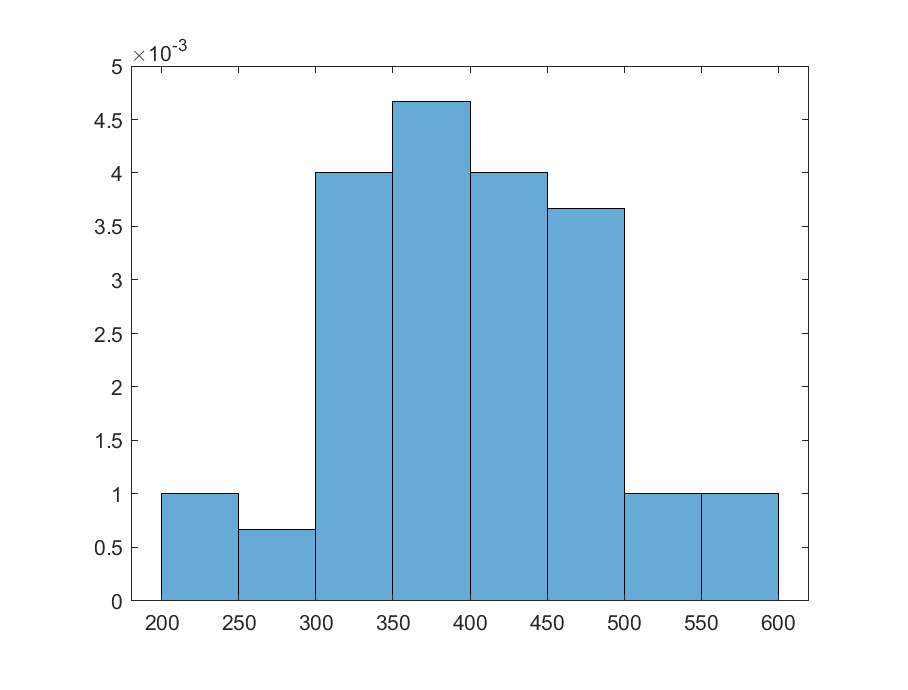
\includegraphics[width = 0.5\textwidth]{images/histogram.eps}

就得到了需要的频率分布直方图.从直方图可以更直观地看到图书馆每日借出图书册数的分布情况.
\end{frame}

\begin{frame}{用样本估计总体分布}
\alert{C、频率折线图}

用$d_1,d_2,\dots,d_k$分别表示频率分布直方图中各矩形上边的中点,在直方图的左边延长出一个分段,分段的中点用$d_0$表示.在直方图的右边也延长出一个分段,分段的中点用$d_{k+1}$表示.

用直线连接$d_0,d_1,\dots,d_{k+1}$就得到了一条折线,这条折线叫做频率折线图.频率折线图也反映出数据频率分布的规律.

下图是例子3.1中图书馆借出图书数据的频率折线图.
\centering
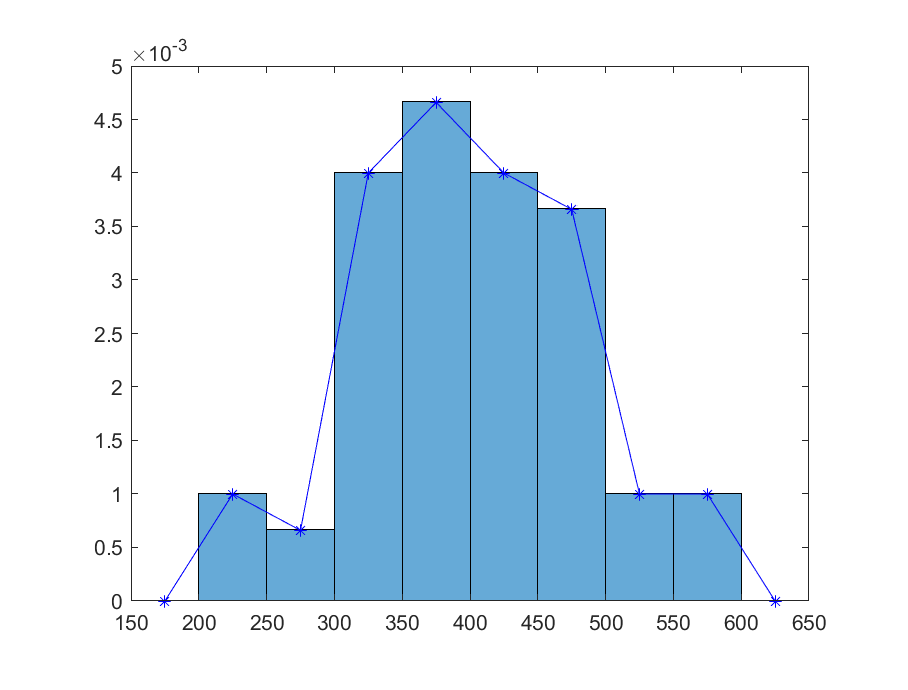
\includegraphics[width = 0.5\textwidth]{images/zhexian.eps}
\end{frame}

	\begin{frame}{用样本估计总体分布}
		\alert{D、数据茎叶图}
		
		直方图主要用于展示分段数据的频率分布,对于没有分段的观测数据还可以用数据的茎叶图展示它的特性.
		
		数据的\alert{茎叶图}由"茎"和"叶"两部分组成,在制作茎叶图的时候要先确定数据的"茎"和"叶".从数据的茎叶图可以看出数据的分布形状以及数据是否对称,是否集中等分布特性.我们通过举例说明茎叶图的制作方法.
		
		例:下面是上海市2004年7月10-31日空气中可吸入颗粒物的监测数据,以这批数据制作茎叶图
		
		85 85 66 71 62 52 55 59 52 62 59 
		70 80 96 97 94 62 51 57 67 96 93
	\end{frame}

	\begin{frame}{用样本估计总体分布}
	解:先将数据从小到大排列得到
	
	51 52 52 55 57 59 59 62 62 62 66 
	67 70 71 80 85 85 93 94 96 96 97\\
	数据的十位上的数是5,6,7,8,9,把他们叫做"茎",排列在下表的第一列,\\
	茎5后面的个位数分别是1,2,2,5,7,9,9,把它们叫做茎5的"叶",排在茎5的后面;\\
	按相同的方法把茎6的叶2,2,2,6,7排在茎6的右边;\\
	$\cdots\cdots\cdots\cdots$\\
	把茎9的叶3,4,6,6,7排在茎9的右边.\\
	就得到了如下的茎叶图
	\end{frame}

	\begin{frame}{用样本估计总体分布}
		$\quad\quad\quad\quad\quad\quad\quad\quad\quad\quad\quad\quad$\begin{tabular}{r|l}
			\hline 茎 & 叶\\
			\hline 5 & 1225799 \\
			\hline 6 & 22267\\
			\hline 7 & 01\\
			\hline 8 & 055\\
			\hline 9 & 34667\\
			\hline
		\end{tabular}
		
		从茎叶图中看出,尽管这22天中可吸入颗粒物都是处于良的水平,但是有较多的时间接近于优,也有较多的时间接近于轻度污染.
		
		数据茎叶图的优点是利用了数据的每个信息,从茎叶图中可以直观地看到数据的分布情况.但是数据量很大时,茎叶图的效果就不好了,因为这是的茎叶图会很长很粗.
	\end{frame}
	
	\begin{frame}{众数和中位数}
		数据的频率分布表、频率分布直方图和茎叶图都可以展示出数据的分布形状,从中可以对数据有一个大致的了解.为了更好地掌握数据的特性和规律,还需要进一步考虑代表数据特征的其他指标.
		\\ \hspace*{\fill} \\
		\alert{A、众数}
		\\ \hspace*{\fill} \\
		我们称观测数据中出现次数最多的数是\alert{众数}(mode),用$M_0$表示.
		
		按照这个定义,在抽样调查中,样本中出现次数最多的数据是样本的众数.
		
		$\quad$如果观测数据中每个数出现的次数都相同,它就没有众数.如果观测数据中有两个或两个以上的数出现次数相同,且出现次数超过其它数的出现次数,这几个数都是众数.
		
		$\quad$众数是观测数据的代表值,它受数据中极大或极小值的影响较小.从分布的角度看,众数出现的频率最高.			
	\end{frame}

	\begin{frame}{(样本)众数和(样本)中位数}
		例子: 某超市用随机抽样的方式调查了30个顾客购买商品的件数,结果从小到大排列如下:
		0,0,1,1,1,2,2,2,3,3,4,5,6,6,8,9,9,10,10,10,10,12,12,13,15,16,18,20,23,29.
		
		求众数和样本均值.
		
		解: 样本中10出现的次数最多,是4次,所以10是众数.样本均值是
		\begin{equation}
			\overline{x} = \frac{1+1+\cdots+23+29}{30} = 8.667.
		\end{equation}
		在此例中,如果购买件数最多的那个顾客购买件数从29增加到40,众数不变,样本均值增加到9.03.
		
		从这个例子中,数据中最大值的变化对众数没有影响,对样本均值的影响较大.
		
		在统计学上,我们将数据的最大值和最小值统一称为极值.称最大值和最小值之差为\alert{极差},$\text{极差} = \text{最大值} - \text{最小值}.$
		
		上例中的极差为$29-0 = 29$,说明所有数据的变化范围或波动幅度不超过29.
	\end{frame}

	\begin{frame}{(样本)众数和(样本)中位数}
		\alert{B、中位数}
		\\ \hspace*{\fill} \\
		设观测数据已经从小到大排列为$x_1\leqslant x_2\leqslant\cdots\leqslant x_n$.
		(1)如果样本量$n$是奇数,我们称中间的数据是\alert{中位数}(median),记作$M_d$.
		\begin{equation}
			M_d = x_m,\text{其中}m = \frac{n+1}{2}.
		\end{equation}
		例如样本1,5,9,12,13的中位数是9.样本4,26,45,67,96,98,112的中位数是67.
		
		(2)如果样本量$n$是偶数,我们称两个中间数据的平均值是中位数,也记作$M_d$.
		\begin{equation}
			M_d = \frac{x_m+x_{m+1}}{2},\text{其中}m = \frac{n}{2}.
		\end{equation}
		例如34,36,45,67,96,98,112,134的中位数是$M_d = (67+96)/2 = 81.5$
	\end{frame}

	\begin{frame}
		由于中位数位于顺序数据的中间,所以有以下性质:
		
		\alert{小于等于中位数的数据不少于样本量的二分之一,大于等于中位数的数据不少于样本量的二分之一}.
		\\ \hspace*{\fill} \\
		例: 2018年,在对A城市工作的某大班同学进行年人均收入(单位:万元)调查时,采用随机抽样的方法得到了以下10个数据:
		
		7.9,9.8,11.7,14.6,16.7,17.9,18.2,19.8,22.6,97.8.
		
		计算中位数和样本均值.
		
		解:数据已经从小到大排列.中位数是$M_d = (16.7+17.9)/2 = 17.3.$
		
		样本均值$\overline{x} = (7.9+9.8+\cdots+97.8) = 23.7.$
		
		在本例中,因为97.8万元的年收入比其他人的年收入高得太多了,所以97.8拉高了样本均值.但是,即使将97.8改为27.8,中位数也不变化.
	\end{frame}

	\begin{frame}{随机对照实验}
		近年来,不断发生的公共安全事故已经成为公众关心的热点.在大洋的彼岸,美国食品药品监督管理局(简称FDA)一直恪守成规,遵照美国的食品和药品法规行事,最大程度地将食品药品安全事故降到最低.尽管如此,在20世纪80年代上市的抗心律失常药Tambocor(氟卡胺)和Enkaid(英卡胺)等还是引发了一次重大药害事件.短短的几年内,估计有5万人因服用这类药物导致心脏骤停而死亡.下面的内容选自[Thomas J. Moore. 《致命的药物》]
	\end{frame}

	\begin{frame}{随机对照实验}
		在20世纪80年代,3M是美国最大的公司之一,曾在财富500强中名列第47位。它因买下一个小型制药公司,再经过10多年的研发,终于有了自己的新药Tambocor(氟卡胺)。新药的上市,成了3M公司的摇钱树。13年来,Tambocor曾在小鼠、大鼠、兔子、猪、狗、猫和狒狒体内进行了试验研究。1975年,FDA批准了Tambocor的临床研究申请,1975-1978年,对于Tambocor的I期和II期临床试验结果比较令人满意。与此同时,百时美公司也加快了同类药品Enkaid(英卡胺)的研发速度。
		
		20世纪70年代,用药物预防心率失常的理论开始流行,尽管缺乏充分的科学依据,1979年医生开出了1200万次处方药,这些事实强烈刺激着3M的Tambocor研发。
		
	\end{frame}

	\begin{frame}{随机对照实验}
		1982年,德国批准了Tambocor的销售。接下来,斯坦福大学的温克医生发表文章讲述了Enkaid导致了一些重症患者的死亡。Tambocor和Enkaid的化学结构相似,但是不一定又相同的问题。温克医生和3M公司讨论Tambocor时,提出在重症患者中试验Tambocor,而3M公司只想在有室性早搏症,且身体健康的人群中试验Tambocor。
		
		1982年11月,3M公司邀请了医学界的专家分析临床试验数据。在45家医院服用Tambocor的患者中,Tambocor没有表现出良好的疗效,反而导致了部分患者的死亡。Enkaid也遇到 了同样的问题。\alert{可惜的是,因为没有统一的试验方案,研究人员很难对于这些数据加以统计分析。}尽管如此,在进一步的试验结果出来之前,3M公司还是按原计划向FDA提交了新药上市的申请。
	\end{frame}

	\begin{frame}{随机对照实验}
		1983年,3M公司在旅游圣地百慕大召开了Tambocor的研讨会,3M支付了全部费用,除了温克医生继续表示担忧外,大部分收了报酬的专家对Tambocor给予热情的支持。
		
		1985年10月8日,在缺乏严密的试验数据的情况下,Tambocor及其同类药物获得上市批准。新一代抗心律失常药开始大量涌向市场。之后,3M借助推销、广告、研讨会等大力推广Tambocor。1988年春,美国的医生每月平均开出57000张Tambocor处方。
		
		1986年12月,FDA批准了Enkaid上市。在一个以市场促销为目的的临床试验中,6周内Enkaid导致了39人死亡。至此,FDA、制药公司和医生都注意到这类药会导致心脏骤停,但是他们认为这些药利大于弊。百时美和3M公司继续开动着赚钱机器。
	\end{frame}

	\begin{frame}{随机对照实验}
		幸运的是,在抗心律失常药被审批和销售的同时,美国心肺血液研究所开始对这类药物进行大规模的心律失常抑制试验(简称CAS试验)。试验包括Tambocor和Enkaid等,涉及4400位患者,27个研究中心和100多家医院,耗时5年,耗资4400万美元。
		
		CAS试验严格按照\alert{随机对照双盲试验}的原则进行:把每个患者随机地分在X组或Y组,为其中一组提供药品,为另一组提供\alert{安慰剂}(貌似药物,但无任何药效)。这是随机对照的含义。不管是研究人员还是患者,除了生物统计学家霍尔斯乔姆一人,没人知道哪些是真药,哪些是安慰剂。这是双盲的含义。谁也没有权利过问治疗组(服用真药的组)和对照组(服用安慰剂的组)的身份情况,由于霍尔斯乔姆默默地保守着秘密,使得想为药品讲话的医生也无从开口,大家只能默默地等待试验的进展。
	\end{frame}	

	\begin{frame}{随机对照实验}
		到1988年9月1日,CAS试验的内部结果如下(其中的猝死人数包括心脏骤停但是抢救成功的患者)。
		
		$\quad\quad\quad\quad\quad\quad\quad\quad\quad$\begin{tabular}{l|l|l}
			\hline  & X组 & Y组\\
			\hline 患者总数 & 576 & 571\\
			\hline 猝死人数 & 3 & 19 \\
			\hline
		\end{tabular}
		
		可以看出,Y组的猝死率是X组的6.38倍。这样的差异大大超出了随机因素所能解释的范围。事实上,对该数据进行如下的假设检验,设原假设H0: 该药物与猝死无关 vs 备择假设H1: 该药物与猝死有关,由调查数据得到:
		
		$\quad\quad\quad\quad\quad\quad\quad$\begin{tabular}{l|l|l}
			\hline 统计量 & 值 & P值 \\
			\hline 卡方 & 12.0068 & 0.0005\\
			\hline 似然比卡方检验 & 13.3432 & 0.0003 \\
			\hline 连续调整卡方 & 10.5612 & 0.0012 \\
			\hline Mantel-Haenszel 卡方 & 11.9963 & 0.0005 \\
			\hline
		\end{tabular}
	\end{frame}	

	\begin{frame}{随机对照实验}
		可以看到,无论是上述的哪一种检验方法,其P值都远小于0.01,所以这个检验是高度显著的,我们可以肯定地说,根据CAS试验,认为该药物与猝死有关时,所犯错误的概率不会超过α=0.01,我们应当否认该药物与猝死无关。随着试验的继续,两组间的差异没有缩小,趋势也没有发生转变。因为患者是被随机分配到X组和Y组的,所以结论表明,不是该药品有效,就是该药品致命。
		
		现在,我们已经知道了,X组是安慰剂组,Y组是试验组。随机对照双盲试验清楚地揭示了Tambocor和Enkaid的确是致命的药物。CAS试验中止后,CAS试验项目长官弗里德曼在给3M公司的信中写道:“采取这个行为是因为Tambocor经证明基本不可能存在疗效,反而它很可能对该患者群体有危害”。
		
	\end{frame}

	\begin{frame}{随机对照实验}
		在CAS试验中,称使用真药的人在试验组,使用安慰剂的人在对照组。通常,实验组由随机选择出的对象构成,试验组的成员接受特殊的待遇或治疗。而对照组由那些没有接受过这种特殊待遇的对象构成,通常为他们提供的是安慰剂。任何好的试验设计应当有一个实验组和对照组。
		
		在CAS试验中,如果没有对照组,为所有的患者提供药品,就无法确认Tambocor和Enkaid会造成心脏骤停的结论。如果试验组和对照组不是随机选择的,由于两组人群的差异,也无法分析出正确的结论。同样,不让医生和患者知道患者在哪一组,甚至不让他们知道安慰剂的存在,是为了得到没有偏见的数据。
	\end{frame}	

	\begin{frame}{随机对照实验}
		当然,随机对照试验也会遇到道德方面的谴责。在决定停止对Tambocor和Enkaid的CAS试验时,就有医生愤怒指责CAS试验“不道德”。因为一旦试验证明药品有效,那么分在对照组的一半人就没有得到治疗。有这样想法的医生并不少。因为当时有一半的医生在治疗心脏早搏,都以为自己在帮助患者。但是,CAS试验的结论证明,他们正在无意中杀害自己的患者。
		
		Rmk:上述抗心律失常药对于部分轻度心律失常患者有效.
		
		随机选择试验对象是英国统计学家Fisher的贡献,在20世纪初,他用此方法致力于农业试验对象的研究。从此,随机选择试验组成为安排试验的基本原则。下面的例子来自[Freedman D.《统计学》]、[Iverson G R, Gergen M.《统计学》]、[Grace N D,et al. The present status of shunts for protal hypertension in cirrhosis. Journal of Gastroenterology.1966,50,686-691]、[Sacks H, Chalmer T C and Smith H. Randomized versus historical controls for clinical trials. American Journal of Medicine,1982,72,233-240]
		
	\end{frame}	
	
	\begin{frame}{随机对照实验}
		例(静脉吻合分流术)在一些肝硬化病例中,许多患者会从肝出血直至死亡.历史上有一种称为"静脉吻合分流术"的外科手术用于治疗肝硬化,其原理是用外科手术的方法使血流改变方向.这种手术花费很大并且有很高的危险性.值得做这样的手术吗?
		
		为了解决上述问题,一共有三批共51次手术试验.第一批进行了32次无对照组的试验.结果如下:
		
		$\quad\quad\quad\quad$\begin{tabular}{|c|c|c|c|c|}
			\hline 设计方法 & 试验次数 & 显著有效 & 中等有效 & 无效\\
			\hline 无对照组 & 32 & 24 & 7 & 1\\
			\hline 所占比例 &    & 75\% & 21.9\% & 3.1\% \\
			\hline
		\end{tabular}
	
		试验说明75\%的手术显著有效,21.9\%的手术中等有效,看来手术是值得做的.
	\end{frame}
	
	\begin{frame}{随机对照实验}
		第二批共进行了15\%次手术试验,这批试验有对照组,但是对照组的患者不是随机选取的.医生根据患者的临床诊断情况决定是将患者编入试验组做手术,还是编入对照组不做手术.结果如下:
		
		$\quad\quad\quad\quad$\begin{tabular}{|c|c|c|c|c|}
			\hline 设计方法 & 试验次数 & 显著有效 & 中等有效 & 无效\\
			\hline 非随机对照 & 15 & 10 & 3 & 2\\
			\hline 所占比例 &    & 66.7\% & 20\% & 13.3\% \\
			\hline
		\end{tabular}
	
		这次试验的结果是66.7\%的手术显著有效,20\%的手术中等有效,13.3\%的手术无效.这个试验结果也是对"静脉吻合分流术"的肯定.这次的结果与无对照组的试验结果差别不是很大.
	\end{frame}
	
	\begin{frame}{随机对照实验}
		再看有随机选取的对照组的第三批试验,这批试验只有4次手术.随机选取的方式类似于掷硬币,如果硬币正面朝上就将患者选入试验组做手术.这次试验的结果如下:
		
		$\quad\quad\quad\quad$\begin{tabular}{|c|c|c|c|c|}
			\hline 设计方法 & 试验次数 & 显著有效 & 中等有效 & 无效\\
			\hline 随机对照 & 4 & 0 & 1 & 3\\
			\hline 所占比例 &    & 0\% & 25\% & 75\% \\
			\hline
		\end{tabular}
	
		随机对照试验的结果显著地否定了外科手术"静脉吻合分流术"的价值.经过认真设计的试验研究显示"静脉吻合分流术"几乎没有什么价值.
	\end{frame}
	
	\begin{frame}{随机对照实验}
		为什么会出现如此大的差别呢?
		
		在无对照组和非随机选取对照组的试验中,试验者根据患者的临床诊断决定是否将他编入试验组进行手术.这样就做出现一种自然的倾向:试验人员更倾向于将那些身体状态较好的患者选入试验组,以减少手术风险.其结果有利于对手术的肯定评价,这种结果是不真实的.
		
		对上述试验的跟踪观测发现,做手术的51个患者中3年后大约有60\%仍然活着,随机对照组中(没做手术的患者)3年后大约也有60\%仍然活着.这说明手术基本是无效的.而在非随机对照组中,只有45\%的患者存活期超过三年,这说明了非随机对照组中的患者健康情况较差,验证了健康情况较好的患者更容易被选入试验组做手术.
		
		随机安排对照组是十分必要的,否则可能得出错误的结论.我们称随机选取试验组的对照试验为\alert{随机对照试验}.在随机对照试验中,为了得到更真实的结果,有时还需要其他的手段配合.
	\end{frame}		
	\begin{frame}{随机对照实验}
		在人类历史上,还有许多成功使用随机对照试验的例子,也有许多惨痛的教训。例如,随机对照试验否定了治疗冠状动脉病的冠状动脉旁道外科手术(该手术费用昂贵),否定了用抗凝剂治疗心脏病突发,否定了用5-FU对结肠癌进行化疗,否定了用己烯雌酚预防流产.具体情况如下:
		\\ \hspace*{\fill} \\%空行
		$\quad\quad\quad$\begin{tabular}{|c|c|c|c|c|}
			\hline 医疗方法 & \multicolumn{2}{|c|}{随机对照试验} & \multicolumn{2}{|c|}{非随机对照试验}\\
			\hline 结论 & 有效 & 无效 & 有效 & 无效 \\
			\hline 冠状旁道外科手术 & 1 & 7 & 16 & 5 \\
			\hline 抗凝剂治疗 & 1 & 9 & 5 & 1 \\
			\hline 5-FU结肠癌化疗 & 0 & 5 & 2 & 0 \\
			\hline 己烯雌酚预防流产 & 0 & 3 & 5 & 0 \\
			\hline
		\end{tabular}
		
	\end{frame}	
		
	\begin{frame}{随机对照实验}	
		特别需要指出的是有关己烯雌酚的试验,随机对照试验完全否定了这种预防流产的药物。而历史上糟糕的非随机对照试验缺赞同药物的疗效,这是一个医学的悲剧。在20世纪60年代末的美国,医生每年大约为5万名孕妇发放这种药。后来揭示,怀孕期间的母亲服用己烯雌酚,20年后将给她们的女儿带来灾害性的副作用,可能引发她们的女儿得一种罕见的癌症。该药于1971年被禁止使用。
		
		人们从太多的悲剧中总结了教训:对一种新药不作随机对照试验是非常危险的。
			
	\end{frame}	
	
	\begin{frame}
		例: 1916年小儿麻痹症(脊髓灰质炎)袭击了美国,以后的40年间,受害者成千上万.20世纪50年代,人们开始发现预防疫苗.当时萨凯(Salk)培育的疫苗最有希望.他的疫苗在试验室表现良好:安全,产生对脊髓灰质炎病毒的抗体.但是在大规模使用前必须进行现场人体试验,通过试验最后确定疫苗是否有效.只有这样才能达到保护儿童的目的.
		
		当时采用了随机对照的研究方案,对每个儿童用类似投掷一个硬币的方法决定是否将他编入试验组:正面朝上分在试验组,否则分在对照组.除了试验的设计人员,连医生也不知道哪个儿童分在试验组,哪个儿童分在对照组.
		
		然后给分在试验组的儿童注射疫苗,给分在对照组的儿童注射生理盐水,让他们认为也被注射了疫苗.得到的结果如下:
		
		$\quad\quad\quad\quad$\begin{tabular}{|c|c|c|}
			\hline & 试验人数 & 试验后的发病率 \\
			\hline 试验组 & 20万 & 28/10万 \\
			\hline 对照组 & 20万 & 71/10万 \\
			\hline
		\end{tabular}
	
		试验结果显示,疫苗将小儿麻痹症的发病率从10万分之71降低到10万分之28.由于71和28的差别超出了随机性本身所能解释的范围,所以宣布疫苗是成功的.进一步的分析指出,可以以近100\%的概率保证疫苗是有效的(见后面的显著性检验一节).
	\end{frame}
	
	\begin{frame}{随机对照实验}
		上例中的安慰剂是注射生理盐水,给对照组的儿童使用安慰剂是为了避免儿童的心理作用影响试验的结果.尽管可以认为仅靠精神作用不能抵抗小儿麻痹症,但是为了确认试验结果的可靠性,使用安慰剂是必要的.
		
		上例中的随机对照试验是双盲的.双盲的之一是指儿童自己不知道自己是在试验组还是在对照组,也就是说不知道自己被注射的是疫苗还是生理盐水(安慰剂),甚至不知道有安慰剂,这就有效地避免了潜在的心理影响.另外一盲是指医生不了解他诊断的患者是在对照组还是在试验组,这就避免了医生对疫苗的主观看法带来的可能影响.在可能的场合,随机对照双盲试验可以最大程度地避免心理因素的影响.
		
		在许多场合,心理因素是不能忽视的.有资料显示在医院中给那些手术后产生剧痛的患者服用用淀粉制成的"止痛片"后,大约有1/3的患者感觉剧痛减轻.		
	\end{frame}

	\begin{frame}
		练习:用$s_x^2$表示$x_1,\dots,x_n$的样本方差,用$b$表示常数,用$s_y^2$表示$y_1,\dots,y_n$的样本方差.当$y_1=x_1+b,y_2=x_2+b,\dots,y_n=x_n+b$时,验证$s_y^2 = s_x^2$.
		\\ \hspace*{\fill} \\%空行
		练习:某学苑超市销售部收到甲乙两厂送来的质地相同的可乐各10瓶,测量后得到甲乙两厂可乐的净含量(单位:ml)分别是:
		$\quad\quad\quad\quad$\begin{tabular}{|c|c|c|c|c|c|c|c|c|c|c|}
			\hline 甲厂 & 501 & 500 & 499 & 500 & 502 & 500 & 500 & 501 & 499 & 498 \\
			\hline 乙厂 & 497 & 501 & 500 & 502 & 499 & 501 & 503 & 500 & 500 & 497 \\
			\hline
		\end{tabular}
	
		问:销售部应当销售哪家的冰可乐.
		\\ \hspace*{\fill} \\%空行
		练习:用自己的话叙述什么是对照组、什么是试验组、什么是随机对照试验.
	\end{frame}
\section{参数的估计方法}
 \frame{\sectionpage}

	\begin{frame}{样本均值和样本方差}
		如果$X$是从总体中随机抽出的个体,则$X$是随机变量,$X$的分布就是总体的分布.如果对总体进行有放回的抽样,则得到独立同分布且和$X$同分布的随机变量$X_1,X_2,\cdots,X_n$.这时称$X_1,X_2,\cdots,X_n$是来自总体$X$的\alert{简单随机样本},简称为总体$X$的\alert{样本}.
		
		$\quad$在观测放射性钋(pō)放射$\alpha$粒子的试验中,用$X$表示7.5s内观测到的粒子数.独立重复观测时,用$X_i$表示第$i$次的观测结果,则$X_1,X_2,\cdots,X_n$独立同分布且和$X$同分布,$X_1,X_2,\cdots,X_n$是总体$X$的样本.
		
		Def1.1 如果$X_1,X_2,\cdots,X_n$独立同分布且和$X$同分布,则称$X$是总体,称$X_1,X_2,\cdots,X_n$是总体$X$的样本,称观测数据的个数$n$为样本量.
	\end{frame}

	\begin{frame}{样本均值和样本方差}
		在实际问题中得到的总是简单随机样本$X_1,X_2,\cdots,X_n$的观测值$x_1,x_2,\cdots,x_n$,人们也称$x_1,x_2,\cdots,x_n$是总体$X$的样本.在统计学中,常常不把$X_1,X_2,\cdots,X_n$与它们的观测值$x_1,x_2,\cdots,x_n$严格区分,这是为了符号使用的方便.当对数据进行统计分析时,用大写的$X_1,X_2,\cdots,X_n$,实际计算时更多地用小写的$x_1,x_2,\cdots,x_n$.
		\\ \hspace*{\fill} \\%空行
		在统计问题中,总体$X$的分布形式往往是已知的.例如重复测量一个物体的重量时,认为总体$X$服从正态分布$N(\mu,\sigma^2)$,未知参数是$\mu,\sigma^2$,问题是根据总体$X$的样本估计总体参数$\mu,\sigma^2$. 观测放射物钋放射$\alpha$粒子时,总体$X$服从泊松分布$\mathcal{P}(\lambda)$,未知参数是$\lambda$,问题是根据总体$X$估计参数$\lambda$.
	\end{frame}

\section{抽样分布}
 \frame{\sectionpage}
	\begin{frame}{抽样分布}
		$\chi^2$分布、$t$分布、$F$分布是统计学中最重要的抽样分布,被称为统计学中的三大分布.本节的任务是推导这三个分布.
		
		抽样分布是统计推断的基础,其理论证明是概率统计课中不可绕过的一个难点.
		
		(1)$\chi^2$分布
		
		设$X_1,...,X_n$是总体$X\sim N(0,1)$的样本,则\alert{平方和
		\begin{equation}
			\xi_n^2 = X_1^2+...+X_n^2
		\end{equation}
		服从$n$个自由度的$\chi^2$分布},有概率密度
		\begin{equation}
			f_n(z) = \frac{1}{2^{n/2}\Gamma(n/2)}z^{n/2-1}e^{-z/2}\bm{1}_{(z>0)}
		\end{equation}
		记作: $\xi_n^2\sim \chi^2(n)$
	\end{frame}

	\begin{frame}
		证明: 往证$Y_k = X_k^2\sim \Gamma(\frac{1}{2},\frac{1}{2})$.
		
		注意到: $\{Y_k = y\} = \{X_k = \sqrt{y}\}\cup\{X_k = -\sqrt{y}\}$,

		故$Y_k$的密度函数是:
		\begin{equation}
			\begin{split}
				f_{Y_k}(y) &= \varphi(\sqrt{y})\frac{1}{2\sqrt{y}} + \varphi(-\sqrt{y})\frac{1}{2\sqrt{y}}\\
				&= \frac{1}{\sqrt{2\pi y}}e^{-y/2}\bm{1}_{(y>0)}.
			\end{split}
		\end{equation}
		这正是$\Gamma(\frac{1}{2},\frac{1}{2})$的概率密度函数,故$Y_k = X_k^2\sim \Gamma(\frac{1}{2},\frac{1}{2})$.
		
		再由$\Gamma$分布的可加性知道:
		\begin{equation}
			\xi_n^2 \sim \Gamma(\frac{n}{2},\frac{1}{2})
		\end{equation}
		因此,它有概率密度函数$f_n(z) = \frac{1}{2^{n/2}\Gamma(n/2)}z^{n/2-1}e^{-z/2}\bm{1}_{(z>0)}$
	\end{frame}

	\begin{frame}	
		另解: 先求分布函数,之后对分布函数求导得概率密度.
		
		$Y_k$有分布函数
		\begin{equation}
		\begin{split}
			F_{Y_k}(y) &= P(X_k^2\leqslant y)  = P(-\sqrt{y}\leqslant X_k\leqslant \sqrt{y}) \\
			&= \varPhi(\sqrt{y}) - \varPhi(-\sqrt{y}) = 2\varPhi(\sqrt{y}) - 1.
		\end{split}
		\end{equation}
		
		因此,
		\begin{equation}
		\begin{split}
			f_{Y_k}(y) &= F_{Y_k}'(y) \\
			&= 2\times\frac{1}{2\sqrt{y}}\varphi(\sqrt{y}) \\
			&= \frac{1}{\sqrt{2\pi y}}e^{-y/2}\bm{1}_{(y>0)}.
		\end{split}
		\end{equation}
		下同第一种解法.
	\end{frame}


	\begin{frame}{$\chi^2$分布}
		\centering
		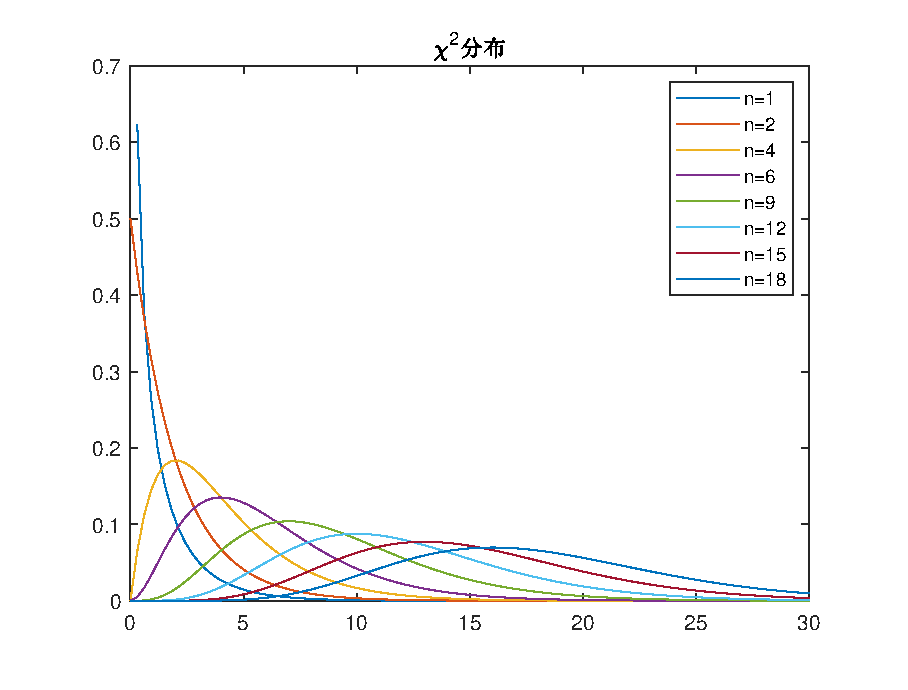
\includegraphics[width = 0.9\textwidth]{images/chi2.eps}
	\end{frame}

	\begin{frame}
		(2)$t$分布
		
		设随机变量$X\sim N(0,1),Y\sim \chi^2(n)$,其中$X,Y$独立,则\alert{随机变量
		\begin{equation}
			T = \frac{X}{\sqrt{Y/n}}
		\end{equation}
		服从n个自由度的$t$分布},并且有概率密度
		\begin{equation}
			f_T(t) = a_n \bigg(1+\frac{t^2}{n}\bigg)^{-\frac{n+1}{2}},
		\end{equation}
		其中$a_n = \frac{1}{\sqrt{n}\mathrm{B}(n/2,1/2)}$是归一化的系数.
	\end{frame}
	
	\begin{frame}{$t$分布}
		证明:(法一)增补变量$S = Y$,来求$(T,S)$的联合概率密度函数$g(t,s)$.
		
		$(X,Y)$有联合密度函数$f(x,y) = \frac{1}{\sqrt{2\pi}}e^{-x^2/2} \frac{1}{2^{n/2}\Gamma(n/2)}y^{n/2-1}e^{-y/2}\bm{1}_{(y>0)}$
		
		注意到: $\{(T,S)=(t,s)\} = \{(X,Y) = (t\sqrt{s/n},s)\}$,
		
		Jacobi阵为:$J = \begin{pmatrix} \sqrt{s/n} & * \\ 0 & 1 \end{pmatrix}$,$|\det(J)| = \sqrt{s/n}$,故有:
		\begin{equation}
			\begin{split}
				g(t,s) &= f(t\sqrt{s/n},s) \sqrt{s/n} \\
				&= \frac{1}{\sqrt{2\pi}}e^{-\frac{t^2s}{2n}} \frac{1}{2^{n/2}\Gamma(n/2)}s^{n/2-1}e^{-s/2}\bm{1}_{(s>0)}\sqrt{s/n} \\
				&= c_n s^{\frac{n-1}{2}}\exp(-\frac{1}{2}(\frac{t^2}{n}+1)s)\bm{1}_{(s>0)}
			\end{split}
		\end{equation}
		因此,$T$的概率密度为$f_T(t) = \int_{0}^{\infty}g(t,s)\mathrm{d}s$
	\end{frame}
	
	\begin{frame}
		为计算该式,替换$u = \frac{1}{2}(\frac{t^2}{n}+1)s$,便有:
		\begin{equation}
			\begin{split}
				f_T(t) &= \int_{0}^{\infty}g(t,s)\mathrm{d}s \\
				&= c_n\int_{0}^{\infty}s^{\frac{n-1}{2}}\exp(-\frac{1}{2}(\frac{t^2}{n}+1)s)\mathrm{d}s \\
				&= 2^{\frac{n-1}2}c_n\bigg[\int_{0}^{\infty}u^{\frac{n-1}{2}}\exp(-u)\mathrm{d}s\bigg] \bigg(1+\frac{t^2}{n}\bigg)^{-\frac{n+1}{2}} \\
				&= a_n \bigg(1+\frac{t^2}{n}\bigg)^{-\frac{n+1}{2}}.
			\end{split}
		\end{equation}
		其中$a_n = 2^{\frac{n-1}2}c_n \Gamma(\frac{n+1}{2}) = \frac{1}{\sqrt{2\pi}}\frac{2^{\frac{n-1}2}}{2^{n/2}\Gamma(n/2)}\frac{1}{\sqrt{n}}\Gamma(\frac{n+1}{2}) = \frac{1}{\sqrt{n}\mathrm{B}(n/2,1/2)}$.
	\end{frame}

	\begin{frame}
		$a_n$的计算也可以由$\int_{-\infty}^{\infty}f_T(t)=1$得到:
		
		\begin{equation}
			\begin{split}
			\frac{1}{a_n} &= 2\int_{0}^{\infty}\bigg(1+\frac{t^2}{n}\bigg)^{-\frac{n+1}{2}}\mathrm{d}t \\
			&= \sqrt{n}\int_{0}^{1}s^{n/2-1}(1-s)^{1/2-1}\mathrm{d}s \big[\text{取变换}1+\frac{t^2}{n}=\frac{1}{s}\big] \\
			&= \sqrt{n}\mathrm{B}(n/2,1/2)
			\end{split}
		\end{equation}
	\end{frame}

	\begin{frame}
		证明:(法二) 先求概率分布,再求导得概率密度.
		
		$(X,Y)$有联合密度函数$f(x,y) = \frac{1}{\sqrt{2\pi}}e^{-x^2/2} \frac{1}{2^{n/2}\Gamma(n/2)}y^{n/2-1}e^{-y/2}\bm{1}_{(y>0)}$
		
		
		\begin{equation}
			\begin{split}
				F_T(t) &= P(T\leqslant t) = \iint\limits_{\{x\leqslant t\sqrt{y/n}\}}f(x,y)\mathrm{d}x\mathrm{d}y \\
				&= \int_{0}^{\infty}\varPhi(t\sqrt{y/n})\frac{1}{2^{n/2}\Gamma(n/2)}y^{n/2-1}e^{-y/2} \mathrm{d}y
			\end{split}
		\end{equation}
		对上式求导得到:
		\begin{equation}
			\begin{split}
				f_T(t) &= F_T'(t) \\
				&= \int_{0}^{\infty}\varphi(t\sqrt{y/n})\sqrt{y/n}\frac{1}{2^{n/2}\Gamma(n/2)}y^{n/2-1}e^{-y/2} \mathrm{d}y \\
				&=\frac{1}{\sqrt{2\pi n}2^{n/2}} \int_{0}^{\infty} y^{\frac{n-1}{2}}\exp(-\frac{1}{2}(\frac{t^2}{n}+1)y) \mathrm{d}y \quad\text{下同法一}
			\end{split}
		\end{equation}
	\end{frame}



	\begin{frame}{$t$分布}
		\centering
		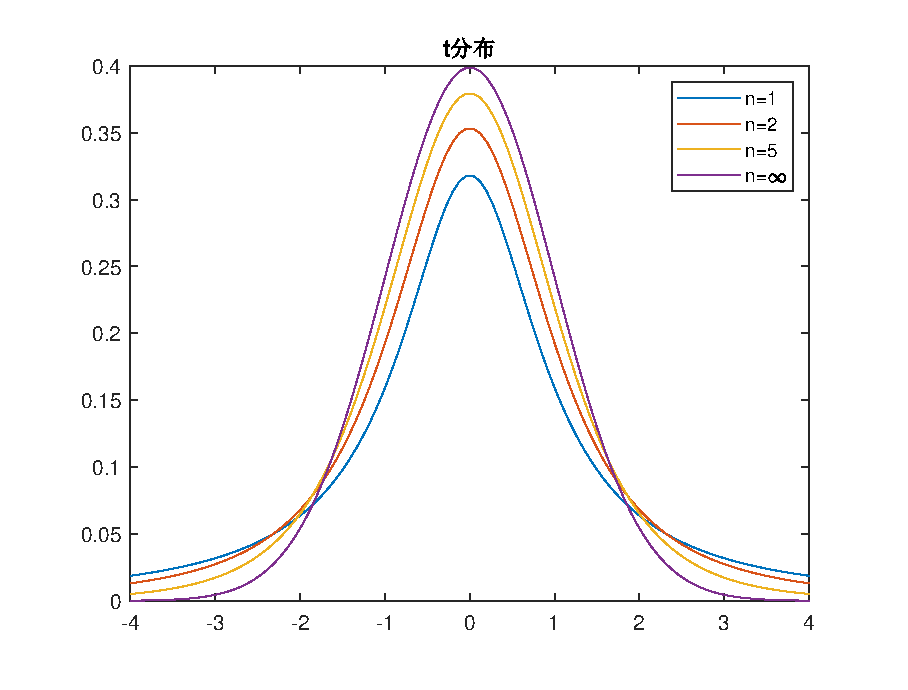
\includegraphics[width = 0.9\textwidth]{images/student(t).eps}
	\end{frame}

	\begin{frame}{$F$分布,注意:分子的自由度在前}
		设$X,Y$独立,分别服从自由度是$n,m$的$\chi^2$分布,则
		\alert{
		\begin{equation}
			Z = \frac{X/n}{Y/m}
		\end{equation}
		服从自由度为$n,m$的$F$分布},有概率密度
		\begin{equation}
			f_Z(z) = cz^{n/2-1}\bigg(1+\frac{nz}{m}\bigg)^{-(n+m)/2}\bm{1}_{(z>0)}.
		\end{equation}
		其中,归一化常数$c = (n/m)^{n/2}[\mathrm{B}(n/2,m/2)]^{-1}$.
	\end{frame}

	\begin{frame}{$F$分布,注意:分子的自由度在前}
		证明:(法一)先求概率分布,再求导得概率密度.
		
		由于$Z = \frac{m}{n}\frac{X}{Y}$,故先计算$U =\frac{X}{Y}$的密度$f_U(u)$,
		
		自然得到$Z$的密度$f_Z(z) = \frac{n}{m}f_U(\frac{n}{m}z)$.
		
		$(X,Y)$有联合密度:$f(x,y) = c_1x^{n/2-1}e^{-x/2}y^{m/2-1}e^{-y/2}\bm{1}_{(x>0,y>0)}$
		
		\begin{equation}
			\begin{split}
				F_U(u) &= P(U\leqslant u) = P(X\leqslant uY) \\
				&= c_1\int_{0}^{\infty} \bigg(\int_{0}^{uy}x^{n/2-1}e^{-x/2}y^{m/2-1}e^{-y/2} \mathrm{d}x\bigg)\mathrm{d}y
			\end{split}
		\end{equation}
		求导得:
		\begin{equation}
		\begin{split}
			f_U(u) &=  c_1\int_{0}^{\infty} y(uy)^{n/2-1}e^{-(uy)/2}y^{m/2-1}e^{-y/2} \mathrm{d}y \\
			&= c_1 \int_{0}^{\infty}u^{n/2-1}y^{(n+m)/2-1}\exp (-\frac{1}{2}(1+u)y) \mathrm{d}y
		\end{split}
		\end{equation} 
	
	\end{frame}


	\begin{frame}
		替换$t = \frac{1}{2}(1+u)y$,计算得到:
		\begin{equation}
			\begin{split}
				f_U(u) &= c_2 [\int_{0}^{\infty} t^{(n+m)/2-1}\exp (-t) \mathrm{d}t][\frac{1}{2}(u+1)]^{-(n+m)/2} u^{n/2-1} \\
				&= c_3 [(u+1)]^{-(n+m)/2} u^{n/2-1}, u>0
			\end{split}
		\end{equation}
		于是知道$Z$的密度
		\begin{equation}
			\begin{split}
				f_Z(z) &= \frac{n}{m}f_U(\frac{n}{m}z) \\
				&= c_4 [(\frac{n}{m}z+1)]^{-(n+m)/2} (\frac{n}{m}z)^{n/2-1}, z>0
			\end{split}
		\end{equation}
	\end{frame}

	\begin{frame}
		常数$c_4$的计算可以按照前面的计算过程一步一步计算下来,也可以利用归一化来计算:
		\begin{equation}
			\begin{split}
				\frac{1}{c_4} &= \int_{0}^{\infty}[(\frac{n}{m}z+1)]^{-(n+m)/2} (\frac{n}{m}z)^{n/2-1}\mathrm{d}z \\
				&=\int_{0}^{1} (\frac{1}{s}-1)^{n/2-1}s^{(n+m)/2}\frac{m}{ns^2}\mathrm{d}s,[1+nu/m=\frac{1}{s}] \\
				&=\frac{m}{n}\int_{0}^{1}(1-s)^{n/2-1}s^{m/2-1}\mathrm{d}s \\
				&=\frac{m}{n}\mathrm{B}(n/2,m/2).
			\end{split}
		\end{equation}
	
	\end{frame}

	\begin{frame}
		(法二):增补变量$W = X+Y$,来求$(Z,W)$的联合概率密度函数$g(z,w)$.
		
		事件\begin{equation}
			\begin{split}
				\{Z=z,W=w\} &= \{\frac{m}{n}\frac{X}{Y}=z,X+Y=w \} \\
				 &= \{ X=\frac{\frac{zn}{m}w}{1+\frac{zn}{m}}, Y =\frac{w}{1+\frac{zn}{m}} \}
			\end{split}
		\end{equation}
		\begin{equation}
			\begin{split}
				|\det(J)| &= \bigg| \det\bigg(\frac{\partial(z,w)}{\partial(x,y)}\bigg) \bigg|^{-1} \\
				&=\bigg| \det \begin{pmatrix} \frac{m}{ny} & -\frac{m}{n}\frac{x}{y^2} \\ 1 & 1 \end{pmatrix}\bigg|^{-1} \\
				&= \frac{n}{m}\frac{y^2}{x+y} = \frac{n}{m}\frac{w}{(1+zn/m)^2}.
			\end{split}
		\end{equation}
	\end{frame}

	\begin{frame}
		因此,得到$(Z,W)$的联合概率密度函数
		\begin{equation}
			\begin{split}
				g(z,w) = f(\frac{\frac{zn}{m}w}{1+\frac{zn}{m}},\frac{w}{1+\frac{zn}{m}})\frac{n}{m}\frac{w}{(1+zn/m)^2},
			\end{split}
		\end{equation}
		其中,$f(x,y)$是$(X,Y)$的概率密度函数.
		将上式经过化简,得到:
		\begin{equation}
			g(z,w) = \frac{1}{2^{\frac{m+n}{2}}\Gamma{\big(\frac{m+n}{2}\big)}}w^{\frac{m+n}{2}-1}e^{-\frac{w}{2}}
			\frac{(n/m)^{n/2}}{\mathrm{B}(m/2,n/2)}z^{n/2-1}(1+\frac{zn}{m})^{-(m+n)/2}
		\end{equation}
		巧了!观察上式发现$g(z,w)$可分离变量,且$(Z,W)$的取值区域为矩形区域.
		
		故随机变量$W$和$Z$独立,
			
		$W$有密度$\frac{1}{2^{\frac{m+n}{2}}\Gamma{\big(\frac{m+n}{2}\big)}}w^{\frac{m+n}{2}-1}e^{-\frac{w}{2}}$.
		
		$Z$有密度$\frac{(n/m)^{n/2}}{\mathrm{B}(m/2,n/2)}z^{n/2-1}(1+\frac{zn}{m})^{-(m+n)/2}$,证毕.
		

		
	\end{frame}

	\begin{frame}{$F$分布,注意:分子的自由度在前}
		\centering
		\includegraphics[width = 0.9\textwidth]{images/fdistribution.eps}
	\end{frame}


	\begin{frame}{抽样分布}
		例: 如果$X\sim \chi^2(n),Y\sim \chi^2(m)$,$X,Y$独立,则$X+Y\sim \chi^2(n+m)$
		
		证明: 取$X_1,X_2,\dots,X_{n+m}$独立同分布,都服从标准正态分布.此时有
		$(X,Y)$和$\big(\sum\limits_{i=1}^{n}X_i^2,\sum\limits_{j=n+1}^{n+m}X_i^2 \big)$同分布,于是
		$X+Y$和$\sum\limits_{i=1}^{n+m}X_i^2$同分布.即有$X+Y\sim \chi^2(n+m)$. 证毕.
		\\ \hspace*{\fill} \\
		例: 设$X_1,\dots,X_n$是来自总体$N(0,1)$的样本.
		\begin{equation}
			\overline{X} = \frac{1}{n}\sum_{j=1}^{n}X_j,\quad S^2 = \frac{1}{n-1}\sum_{j=1}^{n}(X_j-\overline{X})^2
		\end{equation}
		分别是样本均值和样本方差,则
		
		(1) $\overline{X}$和$S^2$独立 \\
		(2) $(n-1)S^2\sim \chi^2(n-1)$.
	\end{frame}
	
	\begin{frame}{抽样分布}
		证明: 引入正交矩阵
		\begin{equation}
			\bm{T} = \frac{1}{\sqrt{n}} 
			\begin{pmatrix} 
				1 & 1 & \dots & 1 \\
				* & * & \dots & * \\ 
				\vdots & \vdots & & \vdots \\
				* & * & \dots & * 
			 \end{pmatrix}.
		\end{equation}
		由$\bm{X}=(X_1,\dots,X_n)^{\mathrm{T}}\sim N(\bm{0},\bm{I})$知道$\bm{Y}=\bm{TX}\sim N(\bm{0},\bm{I}) $,于是$Y_1,\dots,Y_n$独立同分布且都服从于标准正态分布.利用$\overline{X}=Y_1/\sqrt{n}$和
		\begin{equation}
			\sum_{j=1}^{n}X_j^2 = \bm{X}^{\mathrm{T}}\bm{X} = \bm{Y}^{\mathrm{T}}\bm{Y} = 	\sum_{j=1}^{n}Y_j^2
		\end{equation}
	\end{frame}
	
	\begin{frame}{抽样分布}
		得到:
		\begin{equation}
			\begin{split}
				(n-1)S^2 &= \sum_{j=1}^{n}X_j^2 - n\overline{X}^2 \\
				&= \sum_{j=1}^{n}Y_j^2 - Y_1^2 \\
				&= \sum_{j=2}^{n}Y_j^2 \sim \chi^2(n-1)
			\end{split}
		\end{equation}
		并且和$\overline{X}=Y_1/\sqrt{n}$独立.
	\end{frame}

	\begin{frame}{抽样分布}
		\alert{
		练习: 如果$X_1,X_2,\dots,X_n$是总体$N(\mu,\sigma^2)$的样本,证明:
		
		(1) $\overline{X}$和$S^2$独立\\
		(2) $\frac{(n-1)S^2}{\sigma^2}\sim \chi^2(n-1)$.
		}
		证明:
		
		令
		\begin{equation}
			Y_j = \frac{X_j-\mu}{\sigma},
		\end{equation}
		则$Y_1,\dots,Y_n$独立同分布于标准正态分布.
		\begin{equation}
			\overline{X} = \mu + \sigma\overline{Y},\frac{(n-1)S^2}{\sigma^2} = \sum_{j=1}^{n}(Y_j-\overline{Y})^2
		\end{equation}
		由上题的结论知道$\overline{X}$和$S^2$独立,且$\sum_{j=1}^{n}(Y_j-\overline{Y})^2\sim \chi^2(n-1)$.
	\end{frame}

	\begin{frame}

		练习(非中心$\chi^2$分布):如果$X_1,X_2,\dots,X_n$相互独立,$X_i$服从$N(\mu_i,1)$,令$Z=X_1^2+X_2^2+\dots+X_n^2$.证明:
		
		(1) $Z$的概率密度函数为:
		\begin{equation}
		f_Z(z) = e^{-\theta/2}e^{-z/2}\sum_{j=0}^{+\infty}\frac{1}{j!}\frac{(\theta/2)^j}{2^{j+n/2}\Gamma(j+n/2)}z^{j+n/2-1},z>0;
		\end{equation}
		(2)$Z$的特征函数$\mathrm{E}e^{itZ} = \frac{1}{(1-2it)^{n/2}}\exp(\frac{it\theta}{1-2it})$,
		
		其中,$\theta = \mu_1^2+\dots+\mu_n^2>0$.
		\\ \hspace*{\fill} \\%空行
		Rmk:在统计中称$Z$服从自由度为$n$、非中心参数为$\delta = \sqrt{\theta}$的非中心$\chi^2$分布,记作$Z\sim \chi^2(n,\delta)$.
	\end{frame}

	\begin{frame}
		证明:
		
		(1)作正交矩阵
		\begin{equation}
		\bm{T} = \frac{1}{\sqrt{\theta}} 
		\begin{pmatrix} 
		\mu_1 & \mu_2 & \dots & \mu_n \\
		* & * & \dots & * \\ 
		\vdots & \vdots & & \vdots \\
		* & * & \dots & * 
		\end{pmatrix}.
		\end{equation}
		由于$\bm{X} = (X_1,\dots,X_n)^{\mathrm{T}}\sim N(\bm{\mu},\bm{I})$,其中$\bm{\mu}=(\mu_1,\dots,\mu_n)^{\mathrm{T}}$.
		
		令$\bm{Y} = (Y_1,\dots,Y_n) = \bm{TX}$,则$\bm{Y}\sim N(\bm{T\mu},\bm{I})$,因此,有$Y_1,\dots,Y_n$独立, $Y_i\sim N(b_i,1)$,按$\bm{T}$的取法,有:
		$b_1=\sqrt{\theta},b_2=\dots=b_n=0.$		
		
		记$W=\sum\limits_{j=2}^{n}Y_j^2$,则$Z=W+Y_1^2$,其中,$W$与$Y_1^2$独立,而$W\sim\chi^2(n-1),Y_1\sim N(\sqrt{\theta},1)$.
	\end{frame}

	\begin{frame}
		容易算出: $Y_1^2$有密度:
		\begin{equation}
			\begin{split}
				g(x) &= \frac{1}{2\sqrt{2\pi x}}\bigg[\exp(-\frac{(\sqrt{x}-\sqrt{\theta})^2}{2})+\exp(-\frac{(-\sqrt{x}-\sqrt{\theta})^2}{2})\bigg]\bm{1}_{(x>0)} \\
				&= \frac{1}{2\sqrt{2\pi x}} e^{-\theta/2}e^{-x/2}(e^{\sqrt{\theta x}}+e^{-\sqrt{\theta x}})\bm{1}_{(x>0)} \\
				&= \frac{1}{2\sqrt{2\pi }} e^{-\theta/2}e^{-x/2}\sum_{j=0}^{+\infty}\frac{1}{(2j)!}\theta^{j}x^{j-1/2}\bm{1}_{(x>0)}
			\end{split}
		\end{equation}
		
		回忆$W\sim\chi^2(n-1)$的密度函数:
		\begin{equation}
			k_{n-1}(x) = \frac{1}{2^{(n-1)/2}\Gamma(\frac{n-1}{2})}x^{(n-1)/2-1}e^{-x/2}\bm{1}_{(x>0)}
		\end{equation}
	\end{frame}

	\begin{frame}
		按和的密度公式,定出$Z$的概率密度函数为
		\begin{equation}
			\begin{split}
				f_Z(z) &= \int_{-\infty}^{\infty}g(u)k_{n-1}(z-u)\mathrm{d}u \\
				&= \int_{-\infty}^{\infty}\frac{1}{2\sqrt{2\pi }} e^{-\theta/2}e^{-u/2}\sum_{j=0}^{+\infty}\frac{1}{(2j)!}\theta^{j}u^{j-1/2}\bm{1}_{(u>0)} \\
				&\times\frac{1}{2^{(n-1)/2}\Gamma(\frac{n-1}{2})}(z-u)^{(n-1)/2-1}e^{-(z-u)/2}\bm{1}_{(z-u>0)}\mathrm{d}u \\
				&= \int_{0}^{z}\frac{1}{2\sqrt{2\pi }} e^{-\theta/2}e^{-u/2}\sum_{j=0}^{+\infty}\frac{1}{(2j)!}\theta^{j}u^{j-1/2}\\
				&\times\frac{1}{2^{(n-1)/2}\Gamma(\frac{n-1}{2})}(z-u)^{(n-1)/2-1}e^{-(z-u)/2}\mathrm{d}u \bm{1}_{(z>0)}
			\end{split}
		\end{equation}
	\end{frame}

	\begin{frame}
		将上式稍作整理得到:
		\begin{equation}
			\begin{split}
				f_Z(z) &= 
					\frac{1}{2\sqrt{2\pi}}e^{-\frac{\theta}{2}}\frac{1}{2^{\frac{n-1}{2}}\Gamma(\frac{n-1}{2})}\sum_{j=0}^{+\infty}\theta^je^{-z/2} \\
					&\times\int_{0}^{z}u^{j-1/2}(z-u)^{(n-1)/2-1}\mathrm{d}u \bm{1}_{(z>0)}.
			\end{split}
		\end{equation}
		利用Gamma函数和Beta函数的关系:
		\begin{equation}
			\begin{split}
					\int_{0}^{x}y^a(x-y)^b\mathrm{d}y &= x^{a+b+1}\int_{0}^{1}t^a(1-t)^b\mathrm{d}t \\
					&= x^{a+b+1}\mathrm{B}(a+1,b+1) \\
					&= x^{a+b+1}\frac{\Gamma(a+1)\Gamma(b+1)}{\Gamma(a+b+2)}.
			\end{split}
		\end{equation}
	\end{frame}

	\begin{frame}
		化简得到:
		\begin{equation}
			f_Z(z) =e^{-\theta/2}e^{-z/2}\sum_{j=0}^{+\infty}\frac{1}{j!}\frac{(\theta/2)^j}{2^{j+n/2}\Gamma(j+n/2)}z^{j+n/2-1}\bm{1}_{(z>0)}
		\end{equation}
		(2)要计算$Z$的特征函数$\mathrm{E}e^{itZ}$
		
		若用定义
		\begin{equation}
			\mathrm{E}e^{itZ} = \int_{-\infty}^{\infty}f_Z(z)e^{itz}dz
		\end{equation}
		$\longrightarrow$糟糕!
		\\ \hspace*{\fill} \\%空行
		注意到:$Z=X_1^2+X_2^2+\dots+X_n^2$,并且$X_1,X_2,\dots,X_n$相互独立,于是有:
		\begin{equation}
			\mathrm{E}e^{itZ} = \mathrm{E}e^{itX_1^2}\cdots\mathrm{E}e^{itX_n^2}.
		\end{equation}
	\end{frame}

	\begin{frame}
		注意到:$X_{k}^{2}$有特征函数
		\begin{equation}
			\mathrm{E}e^{itX_{k}^{2}}=\int_{-\infty }^{+\infty}{{{e}^{it{{x}^{2}}}}\frac{1}{\sqrt{2\pi }}{{e}^{-\frac{{{(x-{{\mu }_{k}})}^{2}}}{2}}}\mathrm{d}x}=\frac{1}{\sqrt{2\pi }}\int_{-\infty }^{+\infty }{{{e}^{M(x)}}\mathrm{d}x}
		\end{equation}
		
		其中$M(x)=it{{x}^{2}}-\frac{{{(x-{{\mu }_{k}})}^{2}}}{2}=-\frac{(1-2it)}{2}{{(x-\frac{{{\mu }_{k}}}{1-2it})}^{2}}+\frac{i\mu _{k}^{2}t}{1-2it}.$ 
		
		因此,
		\begin{equation}
			\begin{split}
					\mathrm{E}e^{itX_{k}^{2}} &=\frac{1}{\sqrt{2\pi }}\int_{-\infty }^{+\infty }{{{e}^{-\frac{(1-2it)}{2}{{(x-\frac{{{\mu }_{k}}}{1-2it})}^{2}}+\frac{i\mu _{k}^{2}t}{1-2it}}}dx} \\
					&=\frac{1}{\sqrt{2\pi }}{{e}^{\frac{i\mu _{k}^{2}t}{1-2it}}}\int_{-\infty }^{+\infty }{{{e}^{-\frac{(1-2it)}{2}{{y}^{2}}}}dy} \\
					&=\frac{1}{{{(1-2it)}^{1/2}}}\exp \left( \frac{it\mu _{k}^{2}}{1-2it} \right),
			\end{split}
		\end{equation}
		
	\end{frame}

	\begin{frame}
		最后,
		\begin{equation}
			\begin{split}
				\mathrm{E}e^{itZ} &= \mathrm{E}e^{itX_1^2}\cdots\mathrm{E}e^{itX_n^2} \\
				&= \frac{1}{{{(1-2it)}^{n/2}}}\exp \left( \frac{it\theta}{1-2it} \right).
			\end{split}
		\end{equation}
		练习(非中心$t$分布): 设$X\sim N(\delta,1),Y\sim \chi^2(n)$,求$T = \frac{X}{\sqrt{Y/n}}$的密度函数,其中$\delta\in\mathbb{R}$.
		Ans:
		\begin{equation}
			\begin{split}
				h_{n,\delta}(x) &= \frac{n^{n/2}}{\sqrt{\pi}\Gamma(\frac{n}{2})}e^{-\delta^2/2}(n+x^2)^{-(n+1)/2} \\
				&\times \sum_{j=0}^{\infty}\Gamma(\frac{n+j+1}{2})\frac{(\delta x)^j}{j!}(\frac{2}{n+x^2})^{j/2}.
			\end{split}
		\end{equation}
	\end{frame}

	\begin{frame}
		练习(非中心$F$分布):设$X,Y$独立,$X\sim\chi^2(n),Y\sim\chi^2(m,\delta)$,求$Z=\frac{Y/m}{X/n}$的密度函数.
		\\ \hspace*{\fill} \\%空行
		Ans:
		\begin{equation}
			\begin{split}
				f_{m,n,\delta}(x) &= e^{-\delta^2/2}\sum_{j=0}^{\infty}\frac{(\delta^2/2)^j}{j!}n^{n/2}m^{m/2+j} \\
				&\times \frac{\Gamma(\frac{1}{2}(m+n)+j)}{\Gamma(\frac{n}{2})\Gamma(\frac{m}{2}+j)}
				\frac{x^{m/2-1+j}}{(n+mx)^{(m+n)/2+j}}\bm{1}_{(x>0)}.
			\end{split}
		\end{equation}
	\end{frame}

	\begin{frame}
		练习: 设$X\sim\chi^2(2n),n$为正整数,设$a>0$,$Y\sim\mathcal{P}(\frac{a}{2})$(Poisson分布).
		
		证明:
		\begin{equation}
			P(X<a) = P(Y\geqslant n).
		\end{equation}
		证明: \begin{equation}
			P(X<a) = \frac{1}{2^n\Gamma(n)}\int_{0}^{a}x^{n-1}e^{-x/2}\mathrm{d}x
		\end{equation}
		反复利用分部积分公式:
		\begin{equation}
			\begin{split}
				P(X<a) &= \frac{1}{2^n(n-1)!}\int_{0}^{a}x^{n-1}e^{-x/2}\mathrm{d}x \\
				&= \frac{1}{2^n(n-1)!}\int_{x=0}^{a}e^{-x/2}\mathrm{d}\left(\frac{x^n}{n}\right) \\
				&= \frac{a^n}{2^nn!}e^{-a/2}+\frac{1}{2^{n+1}n!}\int_{0}^{a}x^{n}e^{-x/2}\mathrm{d}x \\
				&= \sum_{k=n}^{n+r}\frac{a^k}{2^kk!}e^{-a/2}+\frac{1}{2^{n+r+1}(n+r)!}\int_{0}^{a}x^{n+r}e^{-x/2}\mathrm{d}x.
			\end{split}
		\end{equation}
	\end{frame}

	\begin{frame}
		放缩:
		\begin{equation}
			\begin{split}
				0&<\frac{1}{2^{n+r+1}(n+r)!}\int_{0}^{a}x^{n+r}e^{-x/2}\mathrm{d}x \\ &<\frac{1}{2^{n+r+1}(n+r)!}\int_{0}^{a}x^{n+r}\mathrm{d}x \\
				&=\frac{1}{2^{n+r+1}(n+r)!}\frac{a^{n+r+1}}{n+r+1} \\
				&=\frac{(a/2)^{n+r+1}}{(n+r+1)!}\rightarrow 0(r\rightarrow\infty)
			\end{split}
		\end{equation}
		(回忆:数学分析中的"阶指幂对"原理.	)
		
		令$r\rightarrow\infty$即得结论
	\end{frame}

	\begin{frame}
		练习:把$\chi^2$分布推广到$n$非整数的情况:$Z$服从$\chi^2(a)$分布,则$Z$是有密度
		\begin{equation}
			f_Z(z)=\frac{1}{2^{a/2}\Gamma(a/2)}z^{a/2-1}e^{-z/2}\bm{1}_{(x>0)}
		\end{equation}
		的随机变量.
		证明: 
		\alert{
		\begin{equation}
			\mathrm{E}Z = a,\mathrm{var}Z=2a;
		\end{equation}
		}
		且当$a\rightarrow\infty$时,
		\begin{equation}
			\frac{Z-a}{\sqrt{2a}}\stackrel{d}{\longrightarrow}N(0,1).
		\end{equation}
	\end{frame}

	\begin{frame}
		证明:由$Z$的概率密度
		\begin{equation}
			f(z) = \frac{1}{2^{a/2}\Gamma(a/2)}z^{a/2-1}e^{-z/2},z>0
		\end{equation}
		得到:
		\begin{equation}
			\begin{split}
				\mathrm{E}(Z^k) &= \int_{-\infty }^{\infty}z^kf(z)\mathrm{d}z \\
				&= \int_{0}^{\infty}\frac{1}{2^{a/2}\Gamma(a/2)}z^{a/2+k-1}e^{-z/2}\mathrm{d}z \\
				&= \int_{0}^{\infty}\frac{2^k}{\Gamma(a/2)}t^{a/2+k-1}e^{-t}\mathrm{d}t \\
				&= \frac{2^k\Gamma(a/2+k)}{\Gamma(a/2)}
			\end{split}
		\end{equation}
		因此,$\mathrm{E}Z = a,\mathrm{E}Z^2 = 4(\frac{a}{2}+1)(\frac{a}{2}) =a(a+2),\mathrm{var}Z=2a. $
	\end{frame}

	\begin{frame}
		还注意到:$Z$有特征函数
		\begin{equation}
		\phi_Z(t) = \mathrm{E}e^{itZ} = \frac{1}{\left(1-2it\right)^{a/2}}
		\end{equation}
		因此,随机变量$\frac{Z-a}{\sqrt{2a}}$的特征函数为
		\begin{equation}
		\begin{split}
		\mathrm{E}e^{it\frac{Z-a}{\sqrt{2a}}}&=e^{-it\frac{a}{\sqrt{2a}}}\mathrm{E}e^{i\frac{t}{\sqrt{2a}}Z} = e^{-it\frac{a}{\sqrt{2a}}}\frac{1}{\left(1-2i\frac{t}{\sqrt{2a}}\right)^{a/2}} \\
		&= \exp\left(-it\frac{a}{\sqrt{2a}}-\frac{a}{2}\ln(1-2i\frac{t}{\sqrt{2a}})\right) \\
		&= \exp\left(-it\frac{a}{\sqrt{2a}}+it\frac{a}{\sqrt{2a}}-\frac{a}{2}\frac{1}{2}\frac{4t^2}{2a}+o(\frac{1}{\sqrt{a}})  \right)\\
		&=\exp\left(-\frac{1}{2}t^2+o(\frac{1}{\sqrt{a}})  \right)\rightarrow e^{-\frac{t^2}{2}}
		\end{split}
		\end{equation}证毕.
	\end{frame}

	\begin{frame}
		例: 如果$X_1,\dots,X_n$是总体$N(\mu,\sigma^2)$的样本,则:
		\alert{
			\begin{equation}
				\frac{\overline{X}-\mu}{S/\sqrt{n}}\sim t(n-1).
			\end{equation}
		}
		证明:
		\begin{equation}
			Z = \frac{\overline{X}-\mu}{\sigma/\sqrt{n}}\sim N(0,1),\xi = \frac{n-1}{\sigma^2}S^2\sim\chi^2(n-1).
		\end{equation}
		$Z$和$\xi$独立,于是:
		\begin{equation}
			\frac{\overline{X}-\mu}{S/\sqrt{n}} = \frac{Z}{\sqrt{\xi/(n-1)}}\sim t(n-1).
		\end{equation}
	\end{frame}

	\begin{frame}
		例:设$X_1,\dots,X_n$是来自总体$N(\mu_1,\sigma_1^2)$的样本,$Y_1,\dots,Y_n$是来自总体$N(\mu_2,\sigma_2^2)$的样本,又设这两个总体是相互独立的,则当$m,n\geqslant 2$时,
		\alert{
			\begin{equation}
				\frac{S_X^2/\sigma_1^2}{S_Y^2/\sigma_2^2}\sim F(n-1,m-1).
			\end{equation}
		}
		其中
		\begin{equation}
			S_X^2 = \frac{1}{n-1}\sum_{j=1}^{n}(X_j-\overline{X})^2,S_Y^2 = \frac{1}{m-1}\sum_{j=1}^{m}(Y_j-\overline{Y})^2
		\end{equation}
		证明:由于$(n-1)S_X^2/\sigma_1^2\sim\chi^2(n-1),(m-1)S_Y^2/\sigma_2^2\sim\chi^2(m-1)$且二者独立,
		
		由$F$分布的定义知结论成立.
	\end{frame}

	\begin{frame}
		例:设$X_1,\dots,X_n$是来自总体$X\sim N(\mu_1,\sigma_1^2)$的样本,$Y_1,\dots,Y_n$是来自总体$Y\sim N(\mu_2,\sigma_2^2)$的样本,又设这两个总体是相互独立的,$\{X_i\}$和$\{Y_j\}$的样本均值、样本方差分别为:
		$\overline{X},\overline{Y},S_X^2,S_Y^2$.定义
		\begin{equation}
			S_W^2 = \frac{(n-1)S_X^2+(m-1)S_Y^2}{n+m-2},
		\end{equation}
		则,
		\alert{
			\begin{equation}
				Z=\frac{(\overline{X}-\overline{Y})-(\mu_1-\mu_2)}{\sqrt{\sigma_1^2/n+\sigma_2^2/m}}\sim N(0,1).
			\end{equation}
		}
	
		如果还有条件$\sigma_1^2 = \sigma_2^2 = \sigma^2$,则
		\alert{
			\begin{equation}
				T=\frac{(\overline{X}-\overline{Y})-(\mu_1-\mu_2)}{S_W\sqrt{1/n+1/m}}\sim t(n+m-2).
			\end{equation}
		}
	\end{frame}

	\begin{frame}
		证明:	由于总体$X,Y$独立,所以$X_1,\dots,X_n$与$Y_1,\dots,Y_n$独立.
		根据概率论的知识知道:
		\begin{equation}
			\overline{X}\sim N(\mu_1,\sigma_1^2/n),\overline{Y}\sim N(\mu_2,\sigma_2^2/m)
		\end{equation}
		利用$\overline{X},\overline{Y}$独立得到:
		\begin{equation}
			\overline{X}-\overline{Y} \sim N(\mu_1-\mu_2,\sigma_1^2/n+\sigma_2^2/m)
		\end{equation}
		于是得到$Z\sim N(0,1)$.
		再证$T\sim t(n+m-2)$.利用
		\begin{equation}
			\xi_1 = \frac{(n-1)S_X^2}{\sigma^2}\sim \chi^2(n-1),\xi_2 = \frac{(m-1)S_Y^2}{\sigma^2}\sim \chi^2(m-1),
		\end{equation}
		及$\xi_1,\xi_2$独立,得到:$\xi_1+\xi_2 \sim\chi^2(n+m-2)$.
	\end{frame}

	\begin{frame}
		简单计算,有:
		\begin{equation}
			S_W^2 = \frac{(\xi_1+\xi_2)\sigma^2}{n+m-2}
		\end{equation}
		又由于$Z,\xi_1,\xi_2$相互独立,于是$Z$与$\xi_1+\xi_2$独立.因此,
		\begin{equation}
			T=\frac{(\overline{X}-\overline{Y})-(\mu_1-\mu_2)}{S_W\sqrt{1/n+1/m}} = \frac{Z}{\sqrt{(\xi_1+\xi_2)/(n+m-2)}}\sim t(n+m-2).
		\end{equation}
		证毕.
	\end{frame}

	\begin{frame}
		例: 设$T$服从自由度是$n$的$t$分布,证明:
		若整数$k<n$,则$\mathrm{E}T^k$存在,若$k\geqslant n$,则$\mathrm{E}T^k$不存在.
		
		证明:
		
		研究积分\begin{equation}
			\begin{split}
				I_k &= \int_{-\infty}^{\infty} |t|^kf_T(t)\mathrm{d}t \\
				&= \int_{-\infty}^{\infty} a_n|t|^k\left(1+\frac{t^2}{n}\right)^{-(n+1)/2}\mathrm{d}t
			\end{split}
		\end{equation}
		由于$|t|^k\left(1+\frac{t^2}{n}\right)^{-(n+1)/2}\sim (\frac{1}{n})^{-(n+1)/2}|t|^{-(n+1)+k},(t\rightarrow\infty)$
		根据广义积分的比较审敛法知道:当且仅当$-(n+1)+k<-1$时,上式收敛,由此便得结论.
	\end{frame}

	\begin{frame}
		例:设$T$服从自由度是$n$的$t$分布,计算: \\
		(1)$\mathrm{E}T,(n\geqslant 2)$;\\
		(2)$\mathrm{var}T,(n\geqslant 3)$.
		
		解:(1)由$f_T(t)$关于$t=0$对称得到\alert{$\mathrm{E}T = 0,(n\geqslant 2)$};
		
		(2) 由于$\mathrm{E}T = 0$,所以$\mathrm{var}T = \mathrm{E}T^2$.
		
		将$T$表示成$T=\frac{X}{\sqrt{Y/n}}$,其中$X\sim N(0,1),Y\sim\chi^2(n)$,($X,Y$独立)就有:
		\begin{equation}
			\mathrm{E}T^2 = n\mathrm{E}X^2\mathrm{E}Y^{-1} = n\mathrm{E}Y^{-1}.
		\end{equation}
		前面曾经计算过:
		\begin{equation}
			\mathrm{E}Y^k = \frac{2^k\Gamma(a/2+k)}{\Gamma(a/2)}
		\end{equation}
		取$k=-1$得到:
		\begin{equation}
			\mathrm{E}Y^{-1} = \frac{2^{-1}\Gamma(n/2-1)}{\Gamma(n/2)} = (n-2)^{-1}.
		\end{equation}
		因此,\alert{$\mathrm{var}T = \frac{n}{n-2},(n\geqslant 3)$.}
	\end{frame}

	\begin{frame}
		例: (1)如果$X\sim F(n,m)$,则$X^{-1}\sim F(m,n)$
		
		(2)对$F(n,m)$分布的上$\alpha$分位数$F_{\alpha}(n,m)$,有:
		\alert{
		\begin{equation}
			F_{\alpha}(n,m) = \frac{1}{F_{1-\alpha}(m,n)}
		\end{equation}	
		}
		证明留作习题.
		
		(3)如果$X\sim F_{n,m}$,当$m>2$时,$\mathrm{E}X = \frac{m}{m-2}$.(仅与第二自由度有关)
		
		证明:表示$X = \frac{\xi_1/n}{\xi_2/m},$其中$\xi_1\sim\chi^2(n),\xi_2\sim\chi^2(m)$相互独立,
		\begin{equation}
			\mathrm{E}X = \frac{m}{n}\mathrm{E}\xi_1\mathrm{E}\frac{1}{\xi_2} = \frac{m}{n}n\mathrm{E}\frac{1}{m -_2} = \frac{m}{m-2}
		\end{equation}
	\end{frame}

\section{假设检验}
    
    \frame{\sectionpage}
    
    \begin{frame}{假设检验}
    	假设检验
    \end{frame}
    

% \section*{Acknowledgments}


\section{}
\begin{frame}{}
\centering
\Huge\bfseries
\textcolor{orange}{The End}
\end{frame}
\end{document}
